\documentclass[11pt]{amsart}
\usepackage[T1]{fontenc}
\usepackage{lmodern}
\usepackage{amssymb,amsmath,amsthm,mathtools}
\usepackage[margin=1.15in]{geometry}
\usepackage{microtype}
\usepackage{enumitem}
\usepackage{booktabs}
\usepackage{array}
\usepackage{graphicx}
\usepackage[hidelinks]{hyperref}
\usepackage[nameinlink]{cleveref}

\setlength{\footnotesep}{9pt}
\setlist[enumerate]{leftmargin=2.3em}

\newtheorem{theorem}{Theorem}[section]
\newtheorem{proposition}[theorem]{Proposition}
\newtheorem{lemma}[theorem]{Lemma}
\newtheorem{corollary}[theorem]{Corollary}
\newtheorem{conjecture}[theorem]{Conjecture}
\newtheorem{maintheorem}{Theorem}
\renewcommand{\themaintheorem}{\Alph{maintheorem}}
\theoremstyle{definition}
\newtheorem{definition}[theorem]{Definition}
\newtheorem{question}[theorem]{Question}
\theoremstyle{remark}
\newtheorem{remark}[theorem]{Remark}

\crefname{maintheorem}{Theorem}{Theorems}
\crefname{question}{Question}{Questions}

\newcommand{\QQ}{\mathbb{Q}}
\newcommand{\RR}{\mathbb{R}}
\newcommand{\ZZ}{\mathbb{Z}}
\newcommand{\CC}{\mathbb{C}}
\newcommand{\PP}{\mathbb{P}}
\newcommand{\cO}{\mathcal{O}}
\newcommand{\cA}{\mathcal{A}}
\newcommand{\cD}{\mathcal{D}}
\newcommand{\cX}{\mathcal{X}}
\newcommand{\Hdg}{\operatorname{Hdg}}
\newcommand{\Alg}{\operatorname{Alg}}
\newcommand{\Ab}{\operatorname{Ab}}
\newcommand{\End}{\operatorname{End}}
\newcommand{\Hg}{\operatorname{Hg}}
\newcommand{\MT}{\operatorname{MT}}
\newcommand{\SU}{\operatorname{SU}}
\newcommand{\U}{\operatorname{U}}
\newcommand{\GL}{\operatorname{GL}}
\newcommand{\Pic}{\operatorname{Pic}}
\newcommand{\CH}{\operatorname{CH}}
\newcommand{\cl}{\operatorname{cl}}
\newcommand{\ch}{\operatorname{ch}}
\newcommand{\pr}{\mathrm{pr}}
\newcommand{\st}[1]{\textup{(#1)}}
\newcommand{\HC}{\textup{(HC)}}

\begin{document}

\title[On the Hodge conjecture for Fermat varieties]{On the Hodge conjecture
for Fermat varieties}

\author{Deep Bhattacharjee}
\address{Formerly, Electro-Gravitational Space Propulsion Laboratory (EGSPL),
Bhubaneswar, Odisha 751030, India}
\email{d.bhattacharjee@erl-forschung.de}
\email{itsdeep@live.com}
\urladdr{https://orcid.org/0000-0003-0466-750X}
\thanks{Source, figures and verification code:
\url{https://github.com/creelie/e84hc}, archived on Zenodo under the concept
DOI \href{https://doi.org/10.5281/zenodo.23234362}{10.5281/zenodo.23234362}.
Release v1.4.0, the first with \Cref{thm:fermat114}, has the version DOI
\href{https://doi.org/10.5281/zenodo.23288228}{10.5281/zenodo.23288228}}

\subjclass[2020]{Primary 14C30; Secondary 14C25, 14J70, 14K22, 65G40}
\keywords{Hodge conjecture, Fermat varieties, Abel--Jacobi map, coniveau,
CM abelian varieties, Weil classes, motivated cycles}
\date{October 10, 2026}

\begin{abstract}
We prove the Hodge conjecture for the Fermat varieties of degree $114$ in
every dimension, and more generally of every degree $2^{a}3^{b}19^{c}$ with
$a\le1$, together with their products and the abelian varieties of Fermat
type of these degrees. The new cycles come from families of curves on the
Fermat threefold of degree $114$, through a residue formula for the
derivative of their Abel--Jacobi maps; one of the two residues is certified
by interval arithmetic. We also prove the Hodge conjecture for Fermat
fourfolds of every odd degree, and determine which combinations of the
standard conjectures around the Hodge conjecture imply it.
\end{abstract}

\maketitle

\section{Introduction}\label{sec:intro}

Let $X$ be a smooth complex projective variety. A class in $H^{2p}(X,\QQ)$ is
a \emph{Hodge class} if its image in $H^{2p}(X,\CC)$ lies in $H^{p,p}(X)$, and
it is \emph{algebraic} if it is a rational linear combination of the classes
of subvarieties of codimension~$p$. Algebraic classes are Hodge classes. Hodge
asked for the converse \cite{Hod52}.

\begin{conjecture}[Hodge]\label{conj:hodge}
For every smooth complex projective variety $X$ and every $p\ge0$, every
Hodge class in $H^{2p}(X,\QQ)$ is algebraic.
\end{conjecture}

We write \HC{} for this statement. It holds for $p\le1$ and $p\ge\dim X-1$, so
for every variety of dimension at most three, and it is open in general. The
question in the title has a precise form: \emph{from which of the statements
that the literature has isolated does \HC{} follow?} This paper answers that
question, proves the conditional theorems that the answer allows, and stops
at the first statement on each route that we cannot prove. We do not prove
the Hodge conjecture, and no statement below should be read as a claim that
it holds.\footnote{Here and below a statement is called \emph{proved} when
it is proved in this paper or in refereed work. Results that are available
only as preprints are marked as such where they are used. The one preprint
on which a theorem of this paper depends, \cite{OAI26}, enters only as an
explicit hypothesis.}

\subsection*{The statements}
The following statements are made precise in \Cref{def:statements}.
\begin{itemize}[leftmargin=2.6em]
\item[\st{F2}] The Hodge conjecture for abelian varieties.
\item[\st{F3$'$}] The Hodge conjecture modulo abelian varieties: every Hodge
class on every $X$ is a sum of classes $\Gamma_{*}\gamma$, where $\gamma$ is
a Hodge class on an abelian variety $B$ and $\Gamma$ is an algebraic cycle on
$B\times X$.
\item[\st{L}] The Lefschetz standard conjecture $B(X)$ of Grothendieck
\cite{Gro69}, for every $X$.
\item[\st{M}] Every Hodge class is motivated in the sense of Andr\'e
\cite{And96}.
\item[\st{V}] The variational Hodge conjecture: in a smooth projective
family over a smooth connected base, a flat family of rational classes that
is algebraic on one fibre is algebraic on every fibre.
\item[\st{CM}] The Hodge conjecture for abelian varieties of CM type.
\item[\st{IP}] Propagation from CM points: \st{V} for polarized abelian
schemes and classes that are algebraic on a fibre of CM type.
\end{itemize}
The statement \st{CM} is the main theorem claimed in the preprint
\cite{OAI26}, which has not been refereed. We have not verified its proof,
and \Cref{ssec:cmclaim} says which parts of it we have checked.

\begin{maintheorem}\label{thm:A}
The following are equivalent:
\begin{enumerate}[label=\textup{(\roman*)}]
\item \HC;
\item \st{F2} and \st{F3$'$};
\item \st{L} and \st{F3$'$};
\item \st{V} and \st{F3$'$};
\item \st{CM}, \st{IP} and \st{F3$'$};
\item \st{L} and \st{M}.
\end{enumerate}
\end{maintheorem}

The implications from (ii)--(vi) to (i) combine known theorems of Andr\'e,
Deligne, Abdulali and Milne with two observations of this paper:
\st{F3$'$} implies \st{M} (\Cref{prop:f3m}), and \st{CM} together with
\st{IP} implies \st{F2} (\Cref{prop:cmip}). The theorem is proved in
\Cref{ssec:proofA}. The next theorem says that these are all the ways in
which the conjecture follows from the statements above, together with the
other statements the paper meets: the semiregularity of Schoen's subvariety
(\Cref{q:schoen}), and the Hodge conjecture for Fermat varieties and for the
Weil classes of the split Weil families over $\QQ(\sqrt{-3})$.

\begin{maintheorem}[The routes]\label{thm:B}
Let $S$ be a set of the statements of \Cref{tab:rules} that does not contain
\HC, and suppose that \HC{} follows from $S$ by the implications of
\Cref{tab:rules}. Then
\begin{enumerate}[label=\textup{(\alph*)}]
\item either $S$ contains \st{F3$'$} together with one of \st{F2}, \st{L},
\st{V}, or both of \st{CM} and \st{IP};
\item or $S$ contains both \st{L} and \st{M}.
\end{enumerate}
Each of the five minimal sets so described implies \HC, and each implies
every statement of \Cref{tab:rules} except the semiregularity of Schoen's
subvariety.
\end{maintheorem}

So there are two ways in. One passes through abelian varieties and needs
\st{F3$'$} together with a statement that implies \st{F2}; the other avoids
abelian varieties and assumes \st{L} and \st{M}, which by \Cref{thm:A} is the
Hodge conjecture in another form. In particular \st{F2} and \st{F3$'$} can be
avoided as hypotheses, but never as consequences, and Schoen's subvariety
lies on no route at all (\Cref{cor:bypass}). The routes are drawn in
\Cref{fig:routes}.

\begin{figure}[t]
\centering
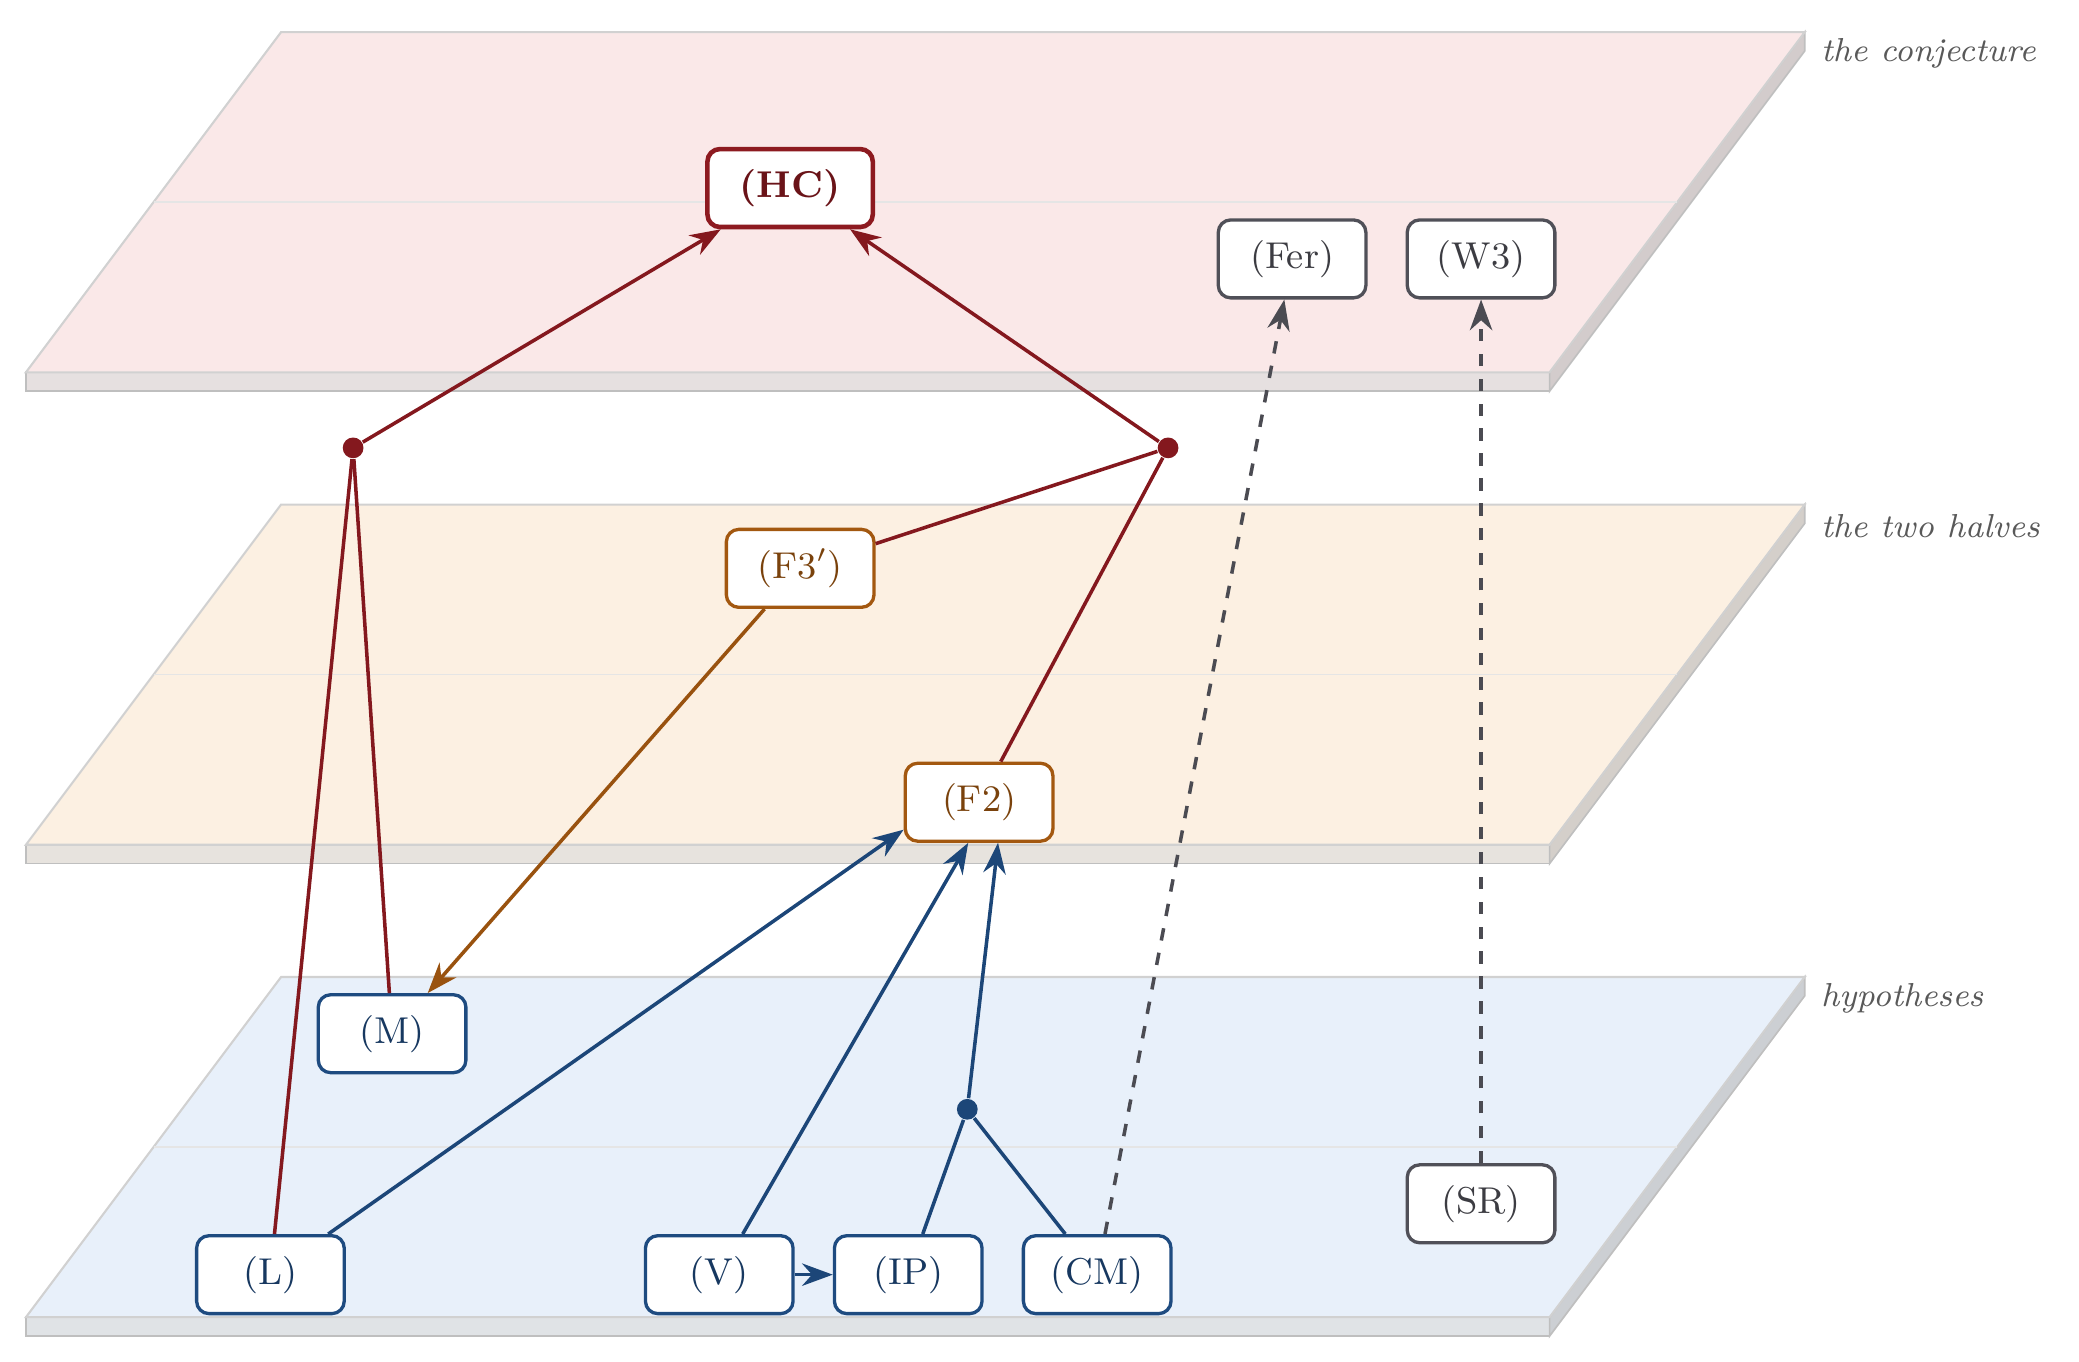
\includegraphics[width=\textwidth]{figures/fig_routes}
\caption{The routes of \Cref{thm:B}. Hypotheses lie on the bottom layer,
the two halves \st{F2} and \st{F3$'$} in the middle, and \HC{} on top.
Arrows are implications of \Cref{tab:rules}. At each dot two lines combine
into a conjunction: $\st{CM}\wedge\st{IP}\Rightarrow\st{F2}$,
$\st{L}\wedge\st{M}\Rightarrow\HC$ and $\st{F2}\wedge\st{F3$'$}\Rightarrow
\HC$. The arrows from \HC{} and \st{F2} to the statements they contain are
not drawn. The dashed arrows on the right lead to the special cases
\st{Fer} and \st{W3} of \Cref{sec:routes}, and not to \HC.}
\label{fig:routes}
\end{figure}

The remaining results are conditional on one statement, or prove one case.
Let $X^{n}_{m}\subseteq\PP^{n+1}$ be the Fermat variety
$x_{0}^{m}+\dots+x_{n+1}^{m}=0$.

\begin{maintheorem}\label{thm:C}
Assume \st{CM}. Then the Hodge conjecture holds for every Fermat variety
$X^{n}_{m}$, for every product of Fermat varieties of any degrees and
dimensions, and for every smooth projective variety onto which such a
product maps surjectively. Without any hypothesis, \st{F3$'$} holds for all
of these varieties.
\end{maintheorem}

Fermat varieties are the first varieties on which the conjecture was
studied in every dimension \cite{Ran80,Shi79}, and unconditional proofs are
known only for special degrees (\Cref{rem:fermatknown}); \Cref{thm:F} below
adds the fourfolds of odd degree. The proof of
\Cref{thm:C} uses the inductive structure of Shioda and Katsura \cite{SK79}
to dominate every Fermat variety by a product of Fermat curves, blown up
along smooth centres, and the fact that Fermat curves have Jacobians of CM
type.

Abelian varieties of Weil type are where \st{F2} is hardest. On the split
Weil family of an imaginary quadratic field over its Shimura variety $S$
(\Cref{ssec:weilfamilies}), write $\Sigma\subseteq S$ for the set of members
on which the Weil classes are algebraic, and $\Sigma_{d}\subseteq\Sigma$ for
the set where they have algebraic representatives of degree at most $d$
(\Cref{def:sigmad}).

\begin{maintheorem}\label{thm:D}
Each $\Sigma_{d}$ is Zariski closed in $S$, and $\Sigma=\bigcup_{d}\Sigma_{d}$.
The following are equivalent:
\begin{enumerate}[label=\textup{(\roman*)}]
\item $\Sigma=S$;
\item $\Sigma_{d}=S$ for some $d$;
\item for some $d$, the CM points in $\Sigma_{d}$ are not contained in any
finite union of proper special subvarieties of $S$.
\end{enumerate}
Under \st{CM} every CM point of $S$ lies in $\Sigma$.
\end{maintheorem}

So under \st{CM} the Weil classes are algebraic on the whole family exactly
when, at the CM points, they have algebraic representatives of uniformly
bounded degree on a set that is not trapped in finitely many proper Shimura
subvarieties. The equivalence of (ii) and (iii) is where the
Andr\'e--Oort conjecture, proved by Pila, Shankar and Tsimerman
\cite{PST21}, enters.

The last result concerns the only cycles known to represent Weil classes at
members with maximal Hodge group in every dimension, those constructed by
Schoen \cite{Sch88}. Let $X$ be a curve of genus $n+1\ge3$, let $C\to X$ be
the \'etale cyclic triple cover given by a line bundle of order three, and
let $B$ be its Prym variety, an abelian variety of dimension $2n$ of Weil
type for $\QQ(\sqrt{-3})$ with polarization class $\eta$.

\begin{maintheorem}\label{thm:E}
There is an irreducible subvariety $Y\subseteq B$ of dimension $n$, built
from one of the three components into which Schoen's cover splits over the
canonical system of $X$, whose class pairs nontrivially with the Weil
classes of $B$. If the Hodge group of $B$ is maximal, which holds for very
general $(X,C)$, then
\[
  \cl(Y)=c\,\eta^{n}+w,\qquad c\in\QQ_{>0},\quad 0\ne w\ \text{a Weil class}.
\]
If $Y$ is semiregular for one such $B$, the Weil classes are algebraic on
every member of the split Weil family of $\QQ(\sqrt{-3})$ in dimension $2n$.
\end{maintheorem}

For $n\le3$ this family is already covered by Schoen's work \cite{Sch88,Sch98}.
For $n\ge4$ it is not: the Prym locus has
dimension $3n$ and the family has dimension $n^{2}$, so $Y$ would have to
deform in $n^{2}-3n$ further directions. The proof of the pairing in \Cref{thm:E} is a short computation with
twisted coefficients on the symmetric product of $X$, and it also gives a
proof of Schoen's theorem that $B$ carries algebraic Weil classes
(\Cref{cor:schoen}). We give the evidence on both sides of \Cref{q:schoen}
in \Cref{ssec:whereitstops}, including a precise analogy
with the Abel--Jacobi curve, which is not semiregular, and with a question
of Markman about a weak form of the semiregularity theorem.

The last result is unconditional.

\begin{maintheorem}\label{thm:F}
Let $m$ be odd. Then the Hodge conjecture holds for the Fermat fourfold
$X^{4}_{m}$.
\end{maintheorem}

By \Cref{prop:fermatchars} the Hodge classes of $X^{4}_{m}$ are spanned by
lines indexed by sextuples of nonzero residues modulo $m$. When $m$ is prime
to $3$, we show that each such sextuple contains two entries $a$ and $-a$,
or is, up to order, $(x,x+m/5,x+2m/5,x+3m/5,x+4m/5,-5x)$
(\Cref{thm:sextuples}). The classes of
the first kind are algebraic by the inductive structure of Shioda and Ran,
and those of the second kind by the cycles of Aoki \cite{Aok87}, pulled back
along a covering of Fermat fourfolds. The proof of the classification uses
the Dirichlet characters modulo the largest order of an entry, and its only
analytic input is the classical fact that $B_{1,\chi}\ne0$ for odd primitive
$\chi$. When $3\mid m$ the classification fails, and we argue by induction
instead (\Cref{ssec:fermatodd}): a sextuple without such a pair either has a
\emph{move}, which trades it, by means of one cycle of Aoki, for a quadruple
or for a sextuple of smaller orders, or it lies in one of three explicit
orbits, in degrees $21$, $33$ and $39$, whose classes we obtain on the
Fermat fourfolds of degrees $21$, $66$ and $78$. When $m$ is prime to $15$,
\Cref{thm:F} follows from Aoki's theorem that every Hodge character then
splits into pairs \cite{Aok83}; it is also known when $m$ is a power of a
prime \cite{Aok87} and when $m=3^{a}5^{b}7^{c}$ \cite{Aok00,Pet26}. In the
remaining degrees it is new for $m>199$, apart from a statement of Kang whose
proof has a gap (\Cref{rem:kang}); smaller degrees were covered by computer
searches (\Cref{rem:fermatknown}). The classification for $m$ prime to $6$,
together with the fact that $B_{1,\chi}\ne0$, has been checked in Lean~4
with Mathlib (\Cref{app:checks}).

\subsection*{What is not proved}
None of the statements \st{F2}, \st{F3$'$}, \st{L}, \st{M}, \st{V},
\st{IP} is proved here, and \st{CM} is used only as a hypothesis. The
Hodge conjecture is open, and by \Cref{cor:bypass} every set of these
statements from which it follows also implies \st{F2} and \st{F3$'$}.
\Cref{sec:end} lists what is proved and what is not, and names the first
open cases: for \st{F2}, the Weil classes of nonsplit abelian sixfolds and
of abelian eightfolds, and the exceptional classes on the square of a
Mumford fourfold; for \st{F3$'$}, the square of a K3 surface with real
multiplication. \Cref{thm:F} does not reach Fermat fourfolds of even
degree: there the method breaks down, because $m/2$ is its own negative and
the subgroups $K_{2}$ of \Cref{ssec:fermatfour} are too small, and Hodge
characters of further kinds occur \cite{Aok83}.

\subsection*{Organization}
\Cref{sec:reductions} proves the reductions that hold for every variety and
defines the statements. \Cref{sec:fermat} proves \Cref{thm:C} and
\Cref{thm:F}.
\Cref{sec:abelian} treats \st{CM} and \st{IP}, proves \Cref{thm:A}, and
proves \Cref{thm:D}. \Cref{sec:weil} proves \Cref{thm:E} and the transfer
theorem for Weil classes. \Cref{sec:routes} proves \Cref{thm:B}.
\Cref{sec:end} collects what is proved and what is not, and
\Cref{app:checks} describes the machine checks of the finite steps. No proof
in this paper depends on a computer.

\subsection*{Conventions}
Varieties are complex, smooth, projective and, unless said otherwise,
connected. Cohomology is singular cohomology with rational coefficients.
For a variety $X$ we write $\Hdg^{p}(X)\subseteq H^{2p}(X,\QQ)$ for the Hodge
classes and $\Alg^{p}(X)\subseteq\Hdg^{p}(X)$ for the algebraic classes. Our
Tate twist is $V(r)^{a,b}=V^{a+r,b+r}$, so that $V(r)$ has weight
$\operatorname{wt}(V)-2r$.

\section{Reductions that hold for every variety}\label{sec:reductions}

\subsection{Correspondences}
Let $B$ and $X$ be varieties, possibly disconnected, with $B$ of pure
dimension $b$. For an algebraic cycle $\Gamma$ of codimension $c$ on
$B\times X$ with rational coefficients, the map
\[
  \Gamma_{*}\colon H^{k}(B,\QQ)\to H^{k+2c-2b}(X,\QQ),\qquad
  y\mapsto\pr_{X*}\bigl(\cl(\Gamma)\cup\pr_{B}^{*}y\bigr),
\]
is a morphism of Hodge structures $H^{k}(B)(b-c)\to H^{k+2c-2b}(X)$. It
carries algebraic classes to algebraic classes, the composite of two such
maps is the map of the composite correspondence, and for a morphism
$f\colon B\to X$ the graph $\Gamma_{f}$ and its transpose give $f_{*}$ and
$f^{*}$ \cite[Chapter~16]{Ful98}. For a cycle with components of several
codimensions we add the maps of the components.

A pure rational Hodge structure $V$ of weight $w$ is \emph{polarizable} if
it carries a bilinear form $Q$ such that $Q(Cx,\bar x)>0$ for $x\ne0$, where
$C$ acts on $V^{a,b}$ by $i^{a-b}$. The cohomology of a variety and its Tate
twists are polarizable, by the Hodge--Riemann relations
\cite[Chapter~6]{Voi02b}. Polarizable Hodge structures are
semisimple.\footnote{If $W\subseteq V$ is a sub-Hodge structure, the
restriction of $Q$ to $W$ is again a polarization, hence nondegenerate, so
$V=W\oplus W^{\perp}$. The orthogonal $W^{\perp}$ is a sub-Hodge structure,
because the decomposition $V_{\CC}=\bigoplus V^{a,b}$ is orthogonal for the
hermitian form $Q(Cx,\bar y)$ and $W_{\CC}$ is the sum of its intersections
with the $V^{a,b}$.}

\begin{lemma}\label{lem:lift}
Let $\varphi\colon V\to W$ be a surjective morphism of polarizable Hodge
structures of weight $2p$. Then $\varphi$ maps the Hodge classes of $V$, the
rational classes of type $(p,p)$, onto those of $W$.
\end{lemma}

\begin{proof}
By semisimplicity the kernel of $\varphi$ has a complement $V'$ that is a
sub-Hodge structure, and $\varphi$ restricts to an isomorphism of Hodge
structures $V'\to W$. Its inverse carries a Hodge class of $W$ to a Hodge
class of $V'\subseteq V$.
\end{proof}

\begin{lemma}[Dominated cohomology]\label{lem:dominated}
Let $X$ be a variety, and let $B_{1},\dots,B_{r}$ be varieties with
algebraic cycles $\Gamma_{j}$ on $B_{j}\times X$, such that the images of
the maps $\Gamma_{j*}$ span $H^{2p}(X,\QQ)$. Then every Hodge class of degree
$2p$ on $X$ is a sum $\sum_{j}\Gamma_{j*}\gamma_{j}$ with $\gamma_{j}$ Hodge
classes on $B_{j}$. In particular, if the Hodge conjecture holds for every
$B_{j}$, it holds for $X$ in degree $2p$.
\end{lemma}

\begin{proof}
Write $\Gamma_{j}=\sum_{c}\Gamma_{j,c}$ with $\Gamma_{j,c}$ of pure
codimension $c$, and $b_{j}=\dim B_{j}$ (if $B_{j}$ is not equidimensional,
treat its components separately). The component $\Gamma_{j,c}$ maps into
degree $2p$ exactly from $H^{k}(B_{j})$ with $k=2p+2b_{j}-2c$, which is
even. The sum of the maps
\[
  \bigoplus_{j,c}H^{2p+2b_{j}-2c}(B_{j},\QQ)(b_{j}-c)\longrightarrow
  H^{2p}(X,\QQ)
\]
is a surjective morphism of polarizable Hodge structures of weight $2p$.
A Hodge class in $H^{2p+2b_{j}-2c}(B_{j})(b_{j}-c)$ is a Hodge class of
$B_{j}$. Apply \Cref{lem:lift}. Algebraic classes go to algebraic classes
under correspondences, which gives the last assertion.
\end{proof}

\subsection{Degree two and hard Lefschetz}

\begin{theorem}[Lefschetz \cite{Lef24}, Kodaira--Spencer \cite{KS53}]\label{thm:lef11}
Every Hodge class of degree two is algebraic.
\end{theorem}

\begin{proof}
The exponential sequence gives an exact sequence
\[
  H^{1}(X,\cO_{X}^{\times})\to H^{2}(X,\ZZ)\to H^{2}(X,\cO_{X}),
\]
whose second
map is the composite of $H^{2}(X,\ZZ)\to H^{2}(X,\CC)$ with the projection
to $H^{0,2}(X)$. An integral class of type $(1,1)$ therefore is the first
Chern class of a holomorphic line bundle, which is algebraic by GAGA, and
its first Chern class is the class of a divisor. A rational Hodge class has
an integral multiple.
\end{proof}

Let $h$ be the class of a hyperplane section of $X$, of dimension $n$, and
$L$ the cup product with $h$. By the hard Lefschetz theorem
$L^{n-k}\colon H^{k}(X,\QQ)\to H^{2n-k}(X,\QQ)$ is an isomorphism for
$k\le n$ \cite[Theorem~6.25]{Voi02b}.

\begin{proposition}\label{prop:hardlef}
For $2p<n$, if every Hodge class of degree $2p$ on $X$ is algebraic, so is
every Hodge class of degree $2n-2p$. Every Hodge class of degree $0$, $2$,
$2n-2$ or $2n$ is algebraic, and \HC{} holds for every variety of dimension
at most three.
\end{proposition}

\begin{proof}
$L^{n-2p}$ maps $H^{p,p}$ onto $H^{n-p,n-p}$ and rational classes to rational
classes, so it maps $\Hdg^{p}(X)$ onto $\Hdg^{n-p}(X)$; and it maps the class
of a subvariety $Z$ to the class of $Z\cap H_{1}\cap\dots\cap H_{n-2p}$ for
general hyperplanes $H_{i}$. Hence
$\Hdg^{n-p}(X)=L^{n-2p}\Alg^{p}(X)\subseteq\Alg^{n-p}(X)$. Degrees $0$ and
$2n$ are spanned by the fundamental class and the class of a point; degree
$2$ is \Cref{thm:lef11}, and degree $2n-2$ follows from it. For $n\le3$
every even degree is one of these.
\end{proof}

\subsection{Surjective morphisms and blow-ups}

\begin{proposition}\label{prop:descent}
Let $f\colon Z\to X$ be a surjective morphism, with $X$ connected, and let
$r=\dim Z-\dim X$. Let $h_{Z}$ be an ample class on $Z$, and $d>0$ the degree
of $h_{Z}^{r}$ on a general fibre. Then $\alpha=d^{-1}f_{*}(h_{Z}^{r}\cup
f^{*}\alpha)$ for every $\alpha\in H^{*}(X,\QQ)$. In particular the
correspondence $\Gamma=d^{-1}(h_{Z}^{r}\times1)\cdot\Gamma_{f}$ from $Z$ to
$X$ satisfies $\Gamma_{*}f^{*}=\mathrm{id}$, so $\Gamma_{*}$ is surjective,
and \HC{} for $Z$ implies \HC{} for $X$.
\end{proposition}

\begin{proof}
By the projection formula
$f_{*}(h_{Z}^{r}\cup f^{*}\alpha)=f_{*}(h_{Z}^{r})\cup\alpha$, and
$f_{*}(h_{Z}^{r})\in H^{0}(X,\QQ)=\QQ$ is the degree $d$, which is positive
because $h_{Z}$ is ample on the fibres. The last claim follows from
\Cref{lem:dominated}.
\end{proof}

\begin{proposition}\label{prop:blowup}
Let $Y\subseteq X$ be a smooth closed subvariety, possibly disconnected, of
codimension $c\ge2$ in every component, let $\pi\colon\tilde X\to X$ be the
blow-up along $Y$, let $j\colon E\to\tilde X$ be the exceptional divisor and
$q\colon E\to Y$ the projective bundle, and let $\xi=c_{1}(\cO_{E}(1))$. Then
\[
  H^{k}(\tilde X,\QQ)=\pi^{*}H^{k}(X,\QQ)\;\oplus\;
  \bigoplus_{i=0}^{c-2}j_{*}\bigl(\xi^{i}\cup q^{*}H^{k-2i-2}(Y,\QQ)\bigr),
\]
and each summand is the image of a correspondence: $\pi^{*}$ from $X$, and
$y\mapsto j_{*}(\xi^{i}\cup q^{*}y)$ from $Y$.
\end{proposition}

\begin{proof}
The decomposition is the blow-up formula \cite[Theorem~7.31]{Voi02b}. The
map $y\mapsto j_{*}(\xi^{i}\cup q^{*}y)$ is the correspondence given by the
image in $Y\times\tilde X$ of a cycle on $E$ representing $\xi^{i}$, pushed
forward along $(q,j)\colon E\to Y\times\tilde X$.
\end{proof}

\subsection{The statements}

\begin{definition}\label{def:statements}
Let $X$ range over all varieties and $p$ over all integers.
\begin{enumerate}[label=\textup{(\arabic*)}]
\item \st{F2}: the Hodge conjecture for every complex abelian
variety.\footnote{In \cite{BhH8} the name \st{F2} denotes a statement about
the Hodge classes not generated by divisors and Weil classes, and it is
proved there to be equivalent to the Hodge conjecture for abelian varieties.
We use the simpler form.}
\item \st{F3$'$}: $\Hdg^{p}(X)=\Ab^{p}(X)$, where $\Ab^{p}(X)$ is the span of
the classes $\Gamma_{*}\gamma$ of degree $2p$ with $B$ an abelian variety
(the point included), $\gamma$ a Hodge class on $B$ and $\Gamma$ an
algebraic cycle on $B\times X$ \cite[Definition~20.34]{BhH8}.
\item \st{L}: for every $X$ and every ample class on $X$, the Lefschetz
involution $*_{L}$ defined below is induced by an algebraic cycle on
$X\times X$. This is Grothendieck's standard conjecture $B(X)$ for every $X$
\cite{Gro69}: by \cite[1.4.4]{Kle68} and \cite[Proposition~1.2]{And96}, the
$\QQ$-algebra of operators generated by $L$ and $*_{L}$ is the one generated by
$L$ and the operator $\Lambda$ of $B(X)$.
\item \st{M}: every Hodge class is motivated in the sense of
\cite[\S1]{And96}.
\item \st{V}: for every smooth projective morphism $f\colon\cX\to S$ over a
smooth connected quasi-projective variety, and every global section $\xi$ of
$R^{2p}f_{*}\QQ$ over $S^{\mathrm{an}}$, if $\xi_{s}$ is algebraic for one
$s\in S$ then $\xi_{t}$ is algebraic for every $t\in S$.
\item \st{CM}: the Hodge conjecture for every abelian variety of CM type.
\item \st{IP}: the case of \st{V} in which $f$ is a polarized abelian scheme
and $\cX_{s}$ is of CM type.
\end{enumerate}
\end{definition}

An abelian variety $A$ is \emph{of CM type} if $\End(A)\otimes\QQ$ contains a
commutative semisimple $\QQ$-algebra of dimension $2\dim A$; the point is of
CM type, and products of abelian varieties of CM type are of CM type.

Each $\Gamma_{*}\gamma$ in \st{F3$'$} is a Hodge class, so
$\Ab^{p}(X)\subseteq\Hdg^{p}(X)$; taking $B$ a point shows that $\Ab^{p}(X)$
contains $\Alg^{p}(X)$. Thus \st{F3$'$} asks only that Hodge classes be
algebraic \emph{modulo} what abelian varieties supply. By
\Cref{prop:descent}, applied to $A\times\PP^{1}\to A$, the conjecture for
varieties that are not abelian already contains the conjecture for abelian
varieties; this is why the half of the conjecture that concerns other
varieties has to be stated modulo abelian varieties to be a separate
problem.

\subsection{The Lefschetz standard conjecture and motivated classes}

Let $X$ have dimension $n$ and ample class $h$. Every class in $H^{k}(X)$ is
uniquely $\sum_{j}L^{j}x_{j}$ with $x_{j}$ primitive of degree $k-2j$, and the
\emph{Lefschetz involution} is defined by $*_{L}(L^{j}x_{j})=L^{n-k+j}x_{j}$
\cite[\S1.1]{And96}. On $H^{k}$ with $k\le n$ it is $L^{n-k}$, and on
$H^{2n-k}$ it is the inverse of $L^{n-k}$. A class $\alpha\in H^{2p}(X,\QQ)$
is \emph{motivated} \cite[D\'efinition~1]{And96} if there are a variety $Y$,
ample classes $h_{X}$ on $X$ and $h_{Y}$ on $Y$, and algebraic classes
$\beta,\gamma$ on $X\times Y$ with
\[
  \alpha=\pr_{X*}\bigl(\beta\cup *_{L}\gamma\bigr),
\]
where $*_{L}$ is the Lefschetz involution of $X\times Y$ for the ample class
$\pr_{X}^{*}h_{X}+\pr_{Y}^{*}h_{Y}$.
We use three facts from \cite{And96}. (a) Motivated classes are Hodge
classes, they contain the algebraic classes, and they form a graded
$\QQ$-algebra that is stable under pull-back and push-forward along
projections \cite[Proposition~2.1 and \S2.5]{And96}; hence a correspondence
given by an algebraic cycle maps motivated classes to motivated
classes.\footnote{For a correspondence, $\Gamma_{*}\gamma=\pr_{X*}(\cl
(\Gamma)\cup\pr_{B}^{*}\gamma)$ is built from $\gamma$ by a pull-back along a
projection, a product with an algebraic class and a push-forward along a
projection.} (b) Every Hodge class on an abelian variety is motivated
\cite[Th\'eor\`eme~0.6.2]{And96}. (c) If the Lefschetz involution of every
variety, for every ample class, is induced by an algebraic cycle, then every
motivated class is algebraic \cite[\S2, after D\'efinition~1]{And96}. Fact
(c) is immediate from the definition: $*_{L}\gamma$ is then the image of an
algebraic class under an algebraic correspondence.

\begin{proposition}\label{prop:LM}
\st{L} and \st{M} together imply \HC.
\end{proposition}

\begin{proof}
By \st{M} every Hodge class is motivated, and by \st{L} and fact~(c) every
motivated class is algebraic.
\end{proof}

\begin{proposition}\label{prop:f3m}
\st{F3$'$} implies \st{M}.
\end{proposition}

\begin{proof}
Under \st{F3$'$} every Hodge class is a sum of classes $\Gamma_{*}\gamma$ with
$\gamma$ a Hodge class on an abelian variety. Such a $\gamma$ is motivated by
fact~(b), and $\Gamma_{*}\gamma$ is motivated by fact~(a).
\end{proof}

\subsection{Families}

\begin{lemma}[Theorem of the fixed part]\label{lem:fixed}
Let $f\colon\cX\to S$ be a smooth projective morphism over a smooth connected
quasi-projective variety, and $\xi$ a global section of $R^{k}f_{*}\QQ$. If
$\xi_{s}$ is a Hodge class for one $s\in S$, then $\xi_{t}$ is a Hodge class
for every $t\in S$.
\end{lemma}

\begin{proof}
By Deligne's theorem of the fixed part \cite[Corollaire~4.1.2]{Del71} the
space $H^{0}(S,R^{k}f_{*}\QQ)$ carries a Hodge structure for which each
restriction $r_{t}\colon H^{0}(S,R^{k}f_{*}\QQ)\to H^{k}(\cX_{t},\QQ)$ is an
injective morphism of Hodge structures.\footnote{Injective because a section
of a local system over a connected base is determined by its value at one
point. The Hodge structure is the image of $H^{k}(\bar\cX,\QQ)\to
H^{k}(\cX_{t},\QQ)$ for a smooth compactification $\bar\cX$ of $\cX$, which
by \cite[4.1.1]{Del71} is the whole invariant part. A global section that is
of type $(p,q)$ at one point is of type $(p,q)$ everywhere
\cite[4.1.3.1]{Del71}.} An injective morphism
of Hodge structures that sends a class $x$ to a class of type $(p,p)$
forces $x$ to be of type $(p,p)$, because it respects the Hodge
decompositions. So $\xi$ is a Hodge class of $H^{0}(S,R^{k}f_{*}\QQ)$, and
$\xi_{t}=r_{t}(\xi)$ is a Hodge class for every $t$.
\end{proof}

\begin{lemma}\label{lem:hcimplies}
\HC{} implies each of \st{F2}, \st{F3$'$}, \st{L}, \st{M}, \st{V}, \st{CM}
and \st{IP}.
\end{lemma}

\begin{proof}
\st{F2} and \st{CM} are special cases, and \st{F3$'$} holds because
$\Ab^{p}(X)$ contains $\Alg^{p}(X)$. For \st{L}: on each $H^{k}(X)$ the involution $*_{L}$ is
a morphism of Hodge structures $H^{k}(X)\to H^{2n-k}(X)(n-k)$, so under the
K\"unneth decomposition and Poincar\'e duality each of its components is a
Hodge class on $X\times X$,\footnote{A $\QQ$-linear map $u\colon H^{a}(X)\to H^{b}(X)$
corresponds to an element of $H^{a}(X)^{\vee}\otimes H^{b}(X)\cong
H^{2n-a}(X)(n)\otimes H^{b}(X)$, a summand of $H^{2n-a+b}(X\times X)(n)$,
and the correspondence it defines acts as $u$. The map $u$ is a morphism of
Hodge structures $H^{a}(X)\to H^{b}(X)(r)$ exactly when this element is a
Hodge class of the appropriate weight.} and \HC{} makes it algebraic.
Algebraic classes are motivated, which gives \st{M}. For \st{V}: if $\xi_{s}$
is algebraic, it is a Hodge class, so $\xi_{t}$ is a Hodge class for every
$t$ by \Cref{lem:fixed}, and \HC{} makes it algebraic. \st{IP} is a case of
\st{V}.
\end{proof}

\section{Fermat varieties}\label{sec:fermat}

\subsection{Varieties dominated by CM abelian varieties}

\begin{definition}\label{def:classD}
Let $\cD$ be the class of varieties $X$, possibly disconnected, such that
$H^{*}(X,\QQ)$ is spanned by the images of maps $\Gamma_{*}\colon
H^{*}(B,\QQ)\to H^{*}(X,\QQ)$, where $B$ runs over the abelian varieties of
CM type, the point included, and $\Gamma$ over the algebraic cycles on
$B\times X$.
\end{definition}

\begin{proposition}\label{prop:classD}
\begin{enumerate}[label=\textup{(\roman*)}]
\item Every $X\in\cD$ satisfies \st{F3$'$}. If \st{CM} holds, every
$X\in\cD$ satisfies \HC.
\item $\cD$ contains every abelian variety of CM type and every finite set of
points, and every curve whose Jacobian is of CM type.
\item $\cD$ is closed under finite disjoint unions, under taking connected
components, and under products.
\item If $Z\in\cD$ and $f\colon Z\to X$ is a surjective morphism, then
$X\in\cD$.
\item If $X\in\cD$ and $Y\subseteq X$ is a smooth closed subvariety of
codimension at least two in every component, with $Y\in\cD$, then the
blow-up of $X$ along $Y$ lies in $\cD$.
\end{enumerate}
\end{proposition}

\begin{proof}
(i) By \Cref{lem:dominated}, applied in each degree to finitely many
$\Gamma_{*}$ whose images span, every Hodge class on $X$ is a sum of classes
$\Gamma_{*}\gamma$ with $\gamma$ a Hodge class on an abelian variety of CM
type. Such a class lies in $\Ab^{p}(X)$, and under \st{CM} it is algebraic.

(ii) For $B$ of CM type take $\Gamma$ the diagonal. For a finite set of
points take $B$ a point and $\Gamma$ the points of $X$ one at a time. For a
curve $C$ with Jacobian $J$ of CM type: $H^{0}(C)$ and $H^{2}(C)$ are spanned
by the fundamental class and the class of a point, which are images from the
point, and $H^{1}(C)=\alpha^{*}H^{1}(J)$ for an Abel--Jacobi map
$\alpha\colon C\to J$, and $\alpha^{*}$ is the correspondence given by the
transpose of the graph of $\alpha$.

(iii) A disjoint union: the cohomology is the direct sum, and a cycle on
$B\times X_{i}$ is a cycle on $B\times\bigsqcup_{i}X_{i}$. A connected
component $X'$ of $X$: restriction $H^{*}(X)\to H^{*}(X')$ is surjective and
is the correspondence given by the transpose of the graph of the inclusion,
so composing gives correspondences from the $B$'s onto $H^{*}(X')$. A
product: by the K\"unneth formula $H^{*}(X\times X')$ is spanned by the
classes $\pr^{*}x\cup\pr'^{*}x'$, and if $x=\Gamma_{*}y$ and
$x'=\Gamma'_{*}y'$ then $\pr^{*}x\cup\pr'^{*}x'=\pm(\Gamma\times\Gamma')_{*}
(\pr_{B}^{*}y\cup\pr_{B'}^{*}y')$, where $\Gamma\times\Gamma'$ is a cycle on
$(B\times B')\times(X\times X')$ and $B\times B'$ is of CM type.

(iv) By (iii) we may assume $X$ connected and replace $Z$ by a component
that maps onto $X$. By \Cref{prop:descent} there is a correspondence $\Gamma$
from $Z$ to $X$ with $\Gamma_{*}$ surjective; composing it with the
correspondences that dominate $H^{*}(Z)$ gives correspondences that dominate
$H^{*}(X)$.

(v) By \Cref{prop:blowup} the cohomology of the blow-up is spanned by the
images of correspondences from $X$ and from $Y$; compose them with the
correspondences that dominate $H^{*}(X)$ and $H^{*}(Y)$.
\end{proof}

\subsection{Fermat curves}

\begin{lemma}\label{lem:fermatcurve}
For every $m\ge1$ the Jacobian of the Fermat curve $X^{1}_{m}$ is of CM type.
\end{lemma}

\begin{proof}
For $m\le2$ the curve is rational and the Jacobian is a point. Let $m\ge3$,
let $g=(m-1)(m-2)/2$ be the genus, and use the affine model $u^{m}+v^{m}=1$,
which is isomorphic to $X^{1}_{m}$ over $\CC$. The group $G=\mu_{m}\times
\mu_{m}$ acts by $(\zeta,\zeta')\cdot(u,v)=(\zeta u,\zeta'v)$, and this action
extends to the smooth projective curve. The forms
\[
  \omega_{r,s}=u^{r-1}v^{s-m}\,du,\qquad r,s\ge1,\quad r+s\le m-1,
\]
are holomorphic\footnote{On the affine curve $v^{s-m}du=-v^{s-1}u^{1-m}dv$
shows that $\omega_{r,s}$ has no poles where $u$ or $v$ is finite. At the
$m$ points at infinity, $u$ and $v$ have simple poles and $du$ has a double
pole, so $\omega_{r,s}$ has order $-(r-1)-(s-m)-2=m-1-r-s\ge0$ there.}, and
there are $(m-1)(m-2)/2=g$ of them, so they form a basis of $H^{1,0}$. The
form $\omega_{r,s}$ is an eigenvector of $G$ with character
$(\zeta,\zeta')\mapsto\zeta^{r}\zeta'^{s}$, and distinct pairs $(r,s)$ give
distinct characters, since $1\le r,s\le m-2$. The complex conjugates span
$H^{0,1}$ and have the characters $(-r,-s)=(m-r,m-s)$; since
$(m-r)+(m-s)\ge m+1$, none of these occurs in $H^{1,0}$. So $H^{1}(X^{1}_{m},
\CC)$ is the direct sum of $2g$ lines on which $G$ acts by $2g$ distinct
characters.

Let $E\subseteq\End(H^{1}(X^{1}_{m},\QQ))$ be the image of the group algebra
$\QQ[G]$. It is commutative and semisimple, as a quotient of a commutative
semisimple algebra, and $E\otimes\CC$ is the image of $\CC[G]$, which acts on
each of the $2g$ lines through its own character; since the characters are
distinct, $E\otimes\CC\cong\CC^{2g}$ and $\dim_{\QQ}E=2g$. The elements of $G$
act on the Jacobian, and $H^{1}$ of the Jacobian is $H^{1}$ of the curve, so
$E\subseteq\End(J)\otimes\QQ$. Thus $J$ is of CM type.
\end{proof}

The characters can be grouped into orbits of $(\ZZ/m)^{\times}$, and each
orbit spans the cohomology of an isogeny factor of $J$ with complex
multiplication by a quotient of $\QQ(\mu_{m})$ \cite{KR78}; this is the
classical computation of Weil \cite{Wei52}.

\subsection{The inductive structure}
Fix $m\ge1$ and write $X^{n}=X^{n}_{m}$, the Fermat variety
$x_{0}^{m}+\dots+x_{n+1}^{m}=0$ in $\PP^{n+1}$, for $n\ge0$; thus $X^{0}$ is a
set of $m$ points. Fix $\varepsilon$ with $\varepsilon^{m}=-1$.

\begin{proposition}[Shioda--Katsura \cite{SK79}]\label{prop:sk}
Let $r,s\ge1$, let $Y\subseteq X^{r}\times X^{s}$ be the subvariety
$x_{r+1}=y_{s+1}=0$, which is isomorphic to $X^{r-1}\times X^{s-1}$ and has
codimension two, and let $Z$ be the blow-up of $X^{r}\times X^{s}$ along $Y$.
The rational map $\varphi\colon X^{r}\times X^{s}\dashrightarrow X^{r+s}$,
\[
  \varphi(x,y)=\bigl[x_{0}y_{s+1}:\dots:x_{r}y_{s+1}:\ \varepsilon x_{r+1}y_{0}:
  \dots:\varepsilon x_{r+1}y_{s}\bigr],
\]
is defined exactly off $Y$, and it extends to a surjective morphism
$Z\to X^{r+s}$.
\end{proposition}

\begin{proof}
The image lies in $X^{r+s}$, because
$y_{s+1}^{m}\sum_{i\le r}x_{i}^{m}+\varepsilon^{m}x_{r+1}^{m}\sum_{j\le s}
y_{j}^{m}=-y_{s+1}^{m}x_{r+1}^{m}+x_{r+1}^{m}y_{s+1}^{m}=0$. All coordinates
vanish exactly on $Y$: if $y_{s+1}\ne0$ they force $x_{0}=\dots=x_{r}=0$ and
then $x_{r+1}^{m}=-\sum_{i\le r}x_{i}^{m}=0$, which is impossible; so
$y_{s+1}=0$, and in the same way $x_{r+1}=0$. On the blow-up, on the chart
where $y_{s+1}=t\,x_{r+1}$, the map is $[t x_{0}:\dots:t x_{r}:\varepsilon
y_{0}:\dots:\varepsilon y_{s}]$; here $y_{0},\dots,y_{s}$ do not all vanish,
because otherwise $y_{s+1}^{m}=0$ as well. The other chart is symmetric. So
$\varphi$ extends to a morphism on $Z$ \cite[Lemma~1.2]{SK79}. It is
dominant, since from a general point of $X^{r+s}$ one recovers
$[x_{0}:\dots:x_{r}]$ and $[y_{0}:\dots:y_{s}]$, and then $x_{r+1}$ and
$y_{s+1}$ up to finitely many choices; its image is closed and $X^{r+s}$ is
irreducible for $r+s\ge2$, so it is surjective.\footnote{Shioda and Katsura
show more: the morphism $Z\to X^{r+s}$ is the composite of the quotient by a
cyclic group of order $m$ and a
birational morphism that contracts two disjoint subvarieties of the quotient
\cite[Theorem~1.7]{SK79}. We use only that it is a surjective morphism.}
\end{proof}

\subsection{Proof of \texorpdfstring{\Cref{thm:C}}{Theorem C}}\label{ssec:proofC}

\begin{theorem}\label{thm:fermatD}
Every Fermat variety $X^{n}_{m}$ lies in $\cD$. So do all products of Fermat
varieties of any degrees and dimensions, and every variety onto which such a
product maps surjectively.
\end{theorem}

\begin{proof}
Fix $m$. We show $X^{n}\in\cD$ by induction on $n$. The set of points
$X^{0}$ lies in $\cD$, and so does the curve $X^{1}$, by
\Cref{prop:classD}(ii) and \Cref{lem:fermatcurve}. Let $n\ge2$ and suppose
$X^{k}\in\cD$ for $k<n$. Apply \Cref{prop:sk} with $r=1$ and $s=n-1$. The
product $X^{1}\times X^{n-1}$ and the centre $Y\cong X^{0}\times X^{n-2}$ lie
in $\cD$ by \Cref{prop:classD}(iii); the blow-up $Z$ lies in $\cD$ by
\Cref{prop:classD}(v); and $X^{n}$, the image of $Z$, lies in $\cD$ by
\Cref{prop:classD}(iv). The remaining assertions are
\Cref{prop:classD}(iii) and~(iv).
\end{proof}

\begin{proof}[Proof of \Cref{thm:C}]
Combine \Cref{thm:fermatD} with \Cref{prop:classD}(i).
\end{proof}

The proof shows more than \Cref{thm:C} states: every Hodge class on a
Fermat variety is the image, under an explicit algebraic correspondence, of a
Hodge class on a power of the Jacobians of Fermat curves of the same degree.
\Cref{thm:C} is therefore exactly as strong as \st{CM} for these powers.

\subsection{The Hodge classes of a Fermat variety}\label{ssec:fermathodge}

The group $G_{n}=\mu_{m}^{n+2}/\mu_{m}$ acts on $X^{n}_{m}$ by multiplying
the coordinates, and its characters are the vectors
$a=(a_{0},\dots,a_{n+1})\in(\ZZ/m)^{n+2}$ with $\sum a_{i}=0$. Let
$\mathfrak{A}^{n}_{m}$ be the set of characters with every $a_{i}\ne0$. For
$a\in\mathfrak{A}^{n}_{m}$ write $\langle a\rangle=\sum_{i}\bar a_{i}/m$,
where $\bar a_{i}\in\{1,\dots,m-1\}$ represents $a_{i}$; it is an integer
between $1$ and $n+1$.

\begin{proposition}\label{prop:fermatchars}
\begin{enumerate}[label=\textup{(\roman*)}]
\item The primitive cohomology $H^{n}_{\mathrm{prim}}(X^{n}_{m},\CC)$ is the
direct sum of lines $V(a)$, one for each $a\in\mathfrak{A}^{n}_{m}$, on which
$G_{n}$ acts by pull-back through the character $a$; and $V(a)\subseteq H^{n-q,q}$ with $q=\langle
a\rangle-1$. Hence
\[
  \dim H^{n}_{\mathrm{prim}}=|\mathfrak{A}^{n}_{m}|
  =\frac{(m-1)^{n+2}+(-1)^{n}(m-1)}{m},\qquad
  h^{n-q,q}_{\mathrm{prim}}=\#\{a:\langle a\rangle=q+1\}.
\]
\item Let $n$ be even. The space of primitive Hodge classes, tensored with
$\CC$, is the sum of the lines $V(a)$ for which $\langle ta\rangle=n/2+1$ for
every $t\in(\ZZ/m)^{\times}$.
\end{enumerate}
\end{proposition}

\begin{proof}
(i) By Griffiths' description of the cohomology of a hypersurface by
residues \cite[\S8]{Gri69}, $H^{n-q,q}_{\mathrm{prim}}(X^{n}_{m})$ is
isomorphic to the graded piece of degree $(q+1)m-(n+2)$ of the Jacobian ring
$\CC[x_{0},\dots,x_{n+1}]/(x_{0}^{m-1},\dots,x_{n+1}^{m-1})$, the class of a
monomial $x^{b}$ corresponding to the residue of $x^{b}\Omega/F^{q+1}$, where
$F=\sum x_{i}^{m}$ and $\Omega=\sum(-1)^{i}x_{i}\,dx_{0}\wedge\cdots\widehat{
dx_{i}}\cdots\wedge dx_{n+1}$. That residue is an eigenvector of $G_{n}$ with
character $a=b+(1,\dots,1)$, because $\Omega$ has character $(1,\dots,1)$
and $F$ is invariant. As $b$ runs over the exponents with $0\le b_{i}\le
m-2$, the vector $a$ runs once over the characters with $1\le\bar a_{i}\le
m-1$; the degree condition is $\sum\bar a_{i}=(q+1)m$, that is,
$\langle a\rangle=q+1$, and it forces $\sum a_{i}=0$ in $\ZZ/m$. The count
of $\mathfrak{A}^{n}_{m}$ follows from the recursion
$N_{k}=(m-1)^{k-1}-N_{k-1}$, $N_{1}=0$, for the number $N_{k}$ of $k$-tuples of
nonzero residues with sum zero.

(ii) The eigenspace decomposition is defined over $\QQ(\mu_{m})$, and the
automorphism $\zeta\mapsto\zeta^{t}$ of $\QQ(\mu_{m})$ carries $V(a)$ to
$V(ta)$. So for each orbit $O$ of $(\ZZ/m)^{\times}$ on
$\mathfrak{A}^{n}_{m}$ the sum $\bigoplus_{a\in O}V(a)$ is defined over $\QQ$,
these rational subspaces decompose $H^{n}_{\mathrm{prim}}(X^{n}_{m},\QQ)$, and
the one for $O$ consists of Hodge classes exactly when every $V(a)$, $a\in O$,
has type $(n/2,n/2)$, that is, when $\langle a\rangle=n/2+1$ on $O$. A
rational class with a component on some $V(a)$ has components on the whole
orbit of $a$, so the Hodge classes are the sum of the rational subspaces of
the orbits of this kind.
\end{proof}

For a Fermat surface the Picard number is
$\rho(X^{2}_{m})=1+\#\{a\in\mathfrak{A}^{2}_{m}:\langle ta\rangle=2\ \text{for
all}\ t\in(\ZZ/m)^{\times}\}$, and $h^{1,1}=(2m^{3}-6m^{2}+7m)/3$.
\Cref{fig:fermat} compares the two for $m\le12$. For $m$ prime to $6$,
$\rho=3(m-1)(m-2)+1$, and the N\'eron--Severi group is spanned by the $3m^{2}$
lines on the surface \cite{AS83}; the quartic, quintic and sextic give
$\rho=20$, $37$ and $86$.

\begin{figure}[t]
\centering
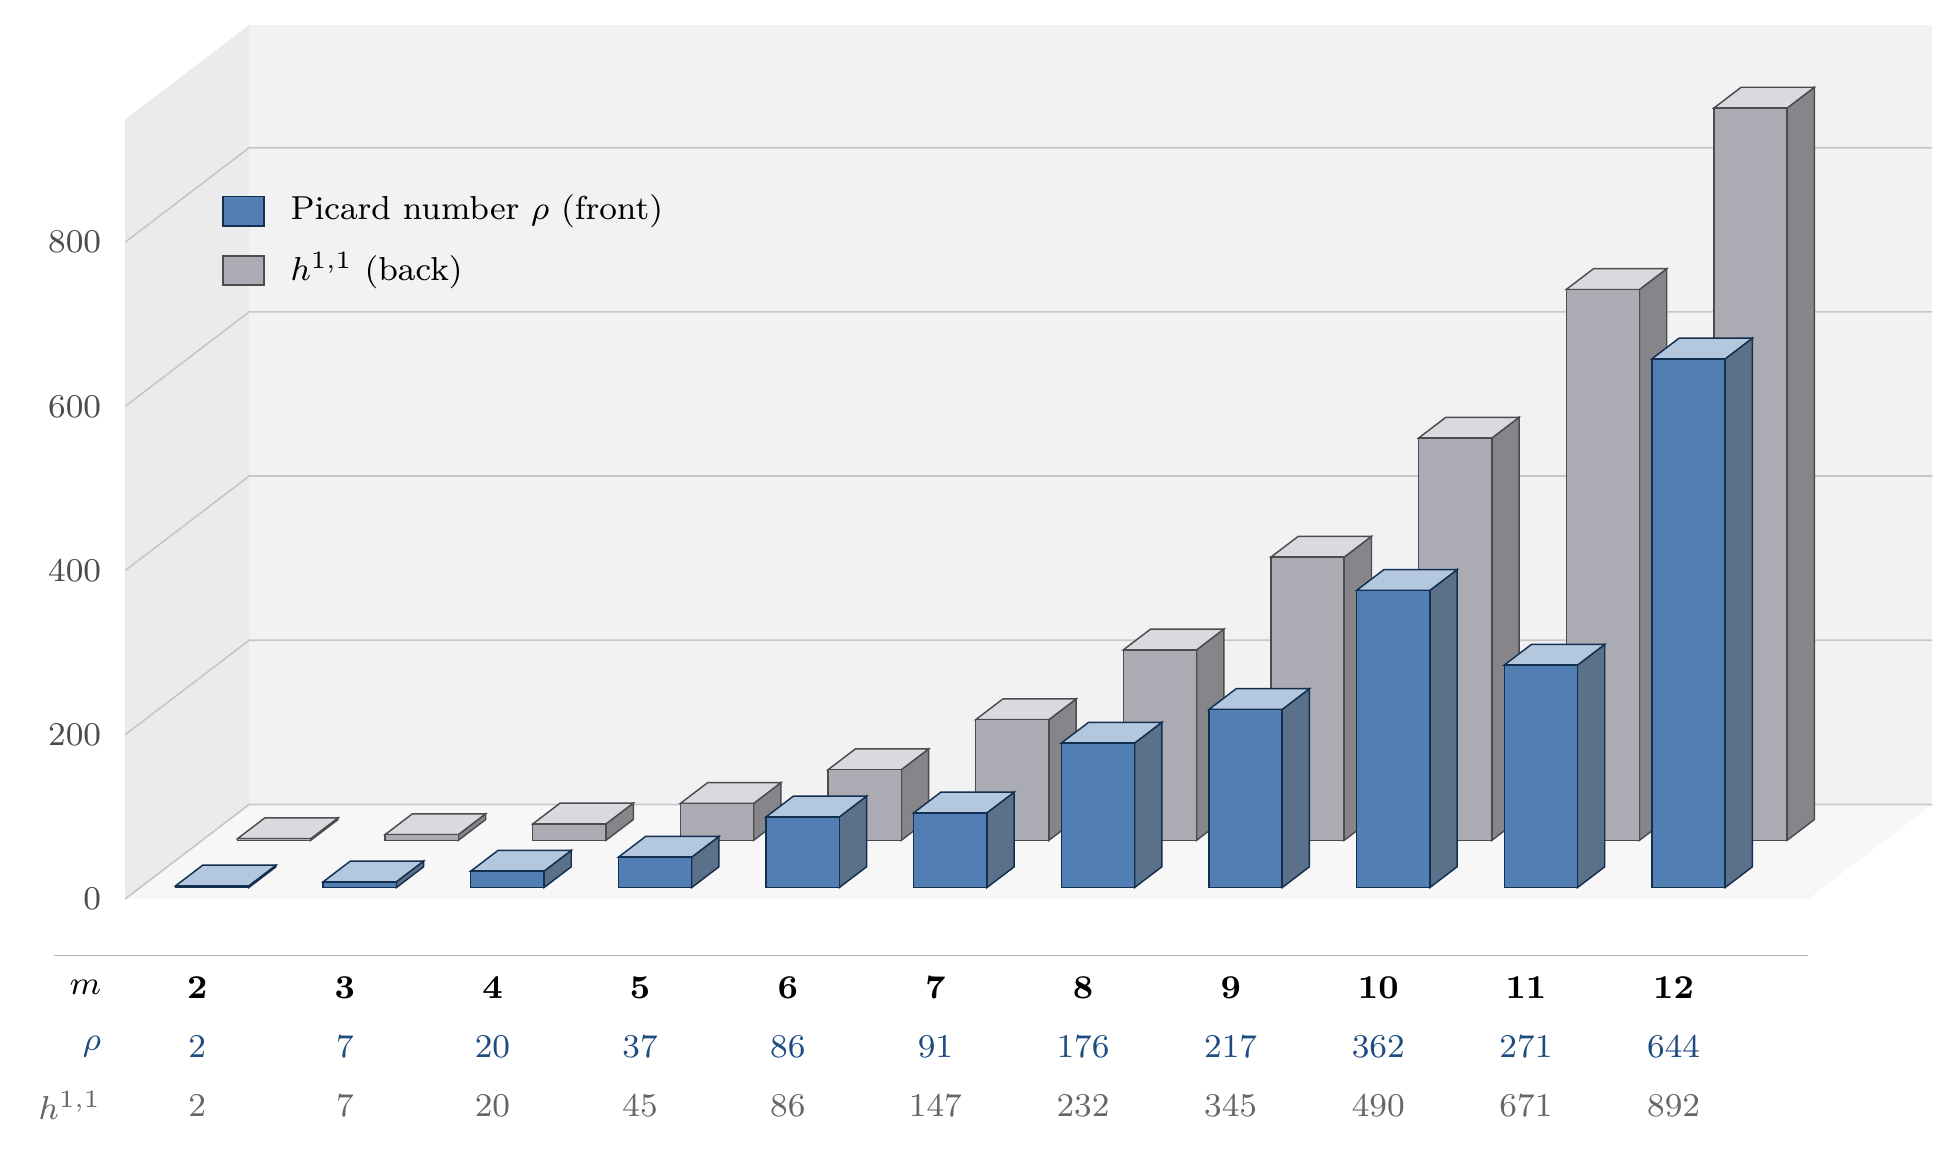
\includegraphics[width=0.92\textwidth]{figures/fig_fermat}
\caption{The Fermat surfaces $X^{2}_{m}$, $2\le m\le12$: the Picard number
$\rho$ (front row) against $h^{1,1}$ (back row), both computed from
\Cref{prop:fermatchars}. On a surface every Hodge class is algebraic
(\Cref{thm:lef11}); the figure shows how the share of $H^{1,1}$ that is
defined over $\QQ$ varies with the arithmetic of $m$. The values of $h^{1,1}$ are recomputed from the Jacobian ring in
Macaulay2 (\Cref{app:checks}).}
\label{fig:fermat}
\end{figure}

\begin{remark}\label{rem:fermatknown}
The Hodge conjecture for $X^{n}_{m}$ is known without hypothesis when $m$ is
prime or $m=4$ \cite{Ran80,Shi79}, when $m\le20$ \cite{Shi79}, and when $m$
is a power of a prime \cite[Corollary~2-3]{Aok87}; see \cite[\S2]{daS21}.
When every prime factor of $m$ exceeds $n+2$, every Hodge character is a
union of pairs \cite[Theorem~A]{Aok83}, and the classes are spanned by linear
subspaces \cite{Ran80,Shi79}; for fourfolds this covers the degrees whose
prime factors are all at least $7$. For fourfolds of degree $m\le100$ prime to
$6$ the conjecture is proved in \cite[Proposition~3.1]{daS21} by a computer
search, and the preprint \cite{Jum26} gives a computer-assisted proof for
fourfolds of odd degree at most $199$. Kang states it for every Fermat
fourfold \cite[Corollary~3.2]{Kan16}, and the preprint \cite{MMRV26}, which
treats all dimensions in degree less than $65$ except $44$, $51$ and $52$,
uses that statement; its proof has the gap described in \Cref{rem:kang}. So
\Cref{thm:F} is new for the degrees $m>199$ prime to $6$ that are divisible by
$5$ and are not powers of $5$, the first of which are $205$, $215$ and $235$,
and its proof, unlike those of \cite{daS21,Jum26}, does not use a computer.
In all these proofs the Hodge classes are written as combinations of the
classes of linear subspaces and of cycles built from them, characters $a$
that split into pairs $a_{i}+a_{j}=0$ corresponding to linear subspaces.
\Cref{thm:C} needs no such decomposition: it moves the whole question to the
Jacobians of Fermat curves. The preprint \cite{OAI26b} announces the Hodge
conjecture on every self-power of a very general member of the family of
diagonal hypersurfaces; the Fermat varieties are special members of that
family.
\end{remark}

\subsection{Fermat fourfolds of degree prime to six}\label{ssec:fermatfour}

In this subsection $m$ is prime to $6$, and we prove \Cref{thm:F}. For
$a\in\ZZ/m$ we write $\bar a\in\{0,\dots,m-1\}$ for its representative,
extending the notation of \Cref{ssec:fermathodge}.

\begin{definition}\label{def:balanced}
Let $A$ be a multiset of nonzero elements of $\ZZ/m$ whose sum is $0$. It is
\emph{balanced} if the integer $\sum_{a\in A}\overline{ta}$ is the same for
every $t\in(\ZZ/m)^{\times}$; we call this integer $h(A)$. It \emph{contains a
pair} if $a\in A$ and $-a\in A$ for some $a$; since $m$ is odd, $a\ne-a$, so
these are two different members of $A$. When $5\mid m$, the \emph{fiber} of
$x\in\ZZ/m$ is the set
\[
  \Phi(x)=\{x+jm/5:\ 0\le j\le4\}
\]
of the five solutions $y$ of $5y=5x$, and $A$ is \emph{$5$-standard} if
$A=\Phi(x)+\{-5x\}$ for some $x$, as multisets.
\end{definition}

For a balanced multiset of $n$ elements, comparing $t$ with $-t$ gives
$h(A)=nm-h(A)$, so $h(A)=nm/2$. By \Cref{prop:fermatchars}(ii), a character
$\alpha\in\mathfrak{A}^{4}_{m}$ spans a line of Hodge classes exactly when
the multiset of its entries is balanced, and the same holds for the
characters $\beta\in\mathfrak{A}^{2}_{m}$ of the Fermat surface. Aoki
writes $\sigma_{5,x}=(x,x+d,x+2d,x+3d,x+4d,-5x)$, $d=m/5$, for the
$5$-standard characters \cite{Aok87}.

\begin{theorem}\label{thm:sextuples}
Let $m$ be prime to $6$.
\begin{enumerate}[label=\textup{(\roman*)}]
\item Every balanced multiset of four nonzero elements of $\ZZ/m$ contains a
pair.
\item Every balanced multiset of six nonzero elements of $\ZZ/m$ contains a
pair or is $5$-standard.
\end{enumerate}
\end{theorem}

Part (i) is Aoki's theorem that the Hodge classes of a Fermat
surface of degree prime to $6$ are spanned by lines \cite[Theorem~A]{Aok83};
we prove it again because the proof of (ii) uses it and runs on the same
lines. When $5\nmid m$, part (ii) says that every Hodge character of
$X^{4}_{m}$ splits into three pairs, which is also contained in
\cite[Theorem~A]{Aok83}, since then every prime factor of $m$ exceeds $6$.
The case $5\mid m$ is new. The theorem has been checked in Lean
(\Cref{app:checks}).

\begin{proof}[Proof of \Cref{thm:F}, given \Cref{thm:sextuples}]
Write $G=G_{4}$ for the group acting on $X=X^{4}_{m}$. By
\Cref{prop:fermatchars}(ii), and since $H^{4}(X,\QQ)$ is the sum of the
primitive part and the line spanned by the square of the hyperplane class,
it is enough to show that every line $V(\alpha)$ with $\alpha$ balanced lies
in $\Alg^{2}(X)\otimes\CC$. Then the Hodge classes and the
algebraic classes span the same complex subspace, and since
$\Alg^{2}(X)\subseteq\Hdg^{2}(X)$ are rational subspaces they are equal. A
subvariety $Z\subseteq X$ \emph{represents} $\alpha$ \cite{Aok87} if the
$\alpha$-component
\[
  \frac{1}{|G|}\sum_{g\in G}\alpha(g)^{-1}g^{*}[Z]=\frac{1}{|G|}\sum_{g\in
  G}\alpha(g)^{-1}[g^{-1}Z]
\]
of $[Z]$ is not zero; it lies in $V(\alpha)$ and in
$\Alg^{2}(X)\otimes\CC$, so then $V(\alpha)\subseteq\Alg^{2}(X)\otimes\CC$.
Permuting the coordinates is an automorphism of $X$ that permutes the lines
$V(\alpha)$ accordingly, so the order of the entries of $\alpha$ does not
matter. By \Cref{thm:sextuples}(ii) there are two cases.

\emph{$\alpha$ contains a pair.} Order the entries as
$\alpha=(\beta_{0},\beta_{1},\beta_{2},\beta_{3},a,-a)$. Since
$\overline{ta}+\overline{-ta}=m$ for every unit $t$, the multiset of entries of
$\beta=(\beta_{0},\dots,\beta_{3})$ is balanced, so $\beta$ is a
Hodge character of the Fermat surface $X^{2}_{m}$, and $V(\beta)$ consists of
algebraic classes by \Cref{thm:lef11}. The character $(a,-a)$ of the set
$X^{0}_{m}$ of $m$ points spans a line of $H^{0}(X^{0}_{m},\CC)$, which is
spanned by classes of points. By the inductive structure, in the form of
Shioda and Ran stated in \cite[Theorem~1-4(i)]{Aok87}, $V(\alpha)$ is then
spanned by algebraic classes.

\emph{$\alpha$ is $5$-standard.} Then $5\mid m$; write $d=m/5$ and
$\alpha=(x,x+d,\dots,x+4d,-5x)$. Aoki constructs a subvariety of
codimension two representing $\alpha$ when $\gcd(\bar x,d)=1$
\cite[Theorem~2-1]{Aok87}. In general let $g=\gcd(\bar x,d)$, $m'=m/g$ and
$d'=d/g=m'/5$. Every entry of $\alpha$ is a multiple of $g$, so
$\alpha=g\alpha'$ with
\[
  \alpha'=(x',x'+d',\dots,x'+4d',-5x')\in(\ZZ/m')^{6},\qquad
  x'=\bar x/g,\quad\gcd(x',d')=1,
\]
where $g\alpha'$ means the image of $\alpha'$ under the injective
homomorphism $\ZZ/m'\to\ZZ/m$, $y\mapsto gy$. The entries of $\alpha'$ are
nonzero, because those of $\alpha$ are. Every unit $t'$ modulo $m'$ lifts to a
unit $t$ modulo $m$, and then $\overline{t'\alpha'_{i}}/m'=\overline{t\alpha
_{i}}/m$ for each $i$; so $\alpha'$ is balanced, and it is a
Hodge character of $X'=X^{4}_{m'}$. In particular $d'\ge3$, since for $d'=1$
one of $x',x'+1,\dots,x'+4$ would vanish modulo $5$. By
\cite[Theorem~2-1]{Aok87} there is a subvariety $Y'\subseteq X'$ of
codimension two that represents $\alpha'$. Let
\[
  \pi\colon X\to X',\qquad[x_{0}:\dots:x_{5}]\mapsto[x_{0}^{g}:\dots:x_{5}^{g}].
\]
It is a finite surjective morphism, and it is equivariant for the homomorphism
$G\to G'$, $\zeta\mapsto\zeta^{g}$, to the group $G'$ acting on $X'$. For
$\xi\in V(\alpha')$ and $\zeta\in G$ we get $\zeta^{*}\pi^{*}\xi=\pi^{*}
(\zeta^{g})^{*}\xi=\alpha'(\zeta^{g})\pi^{*}\xi=\alpha(\zeta)\pi^{*}\xi$, so
$\pi^{*}$ maps $V(\beta')$ into $V(g\beta')$ for every character $\beta'$ of
$G'$, and distinct $\beta'$ go to distinct $g\beta'$. As $\pi_{*}\pi^{*}$ is
multiplication by $\deg\pi$, the map $\pi^{*}$ is injective on cohomology.
Hence the $\alpha$-component of $\pi^{*}[Y']$, the class of the cycle
$\pi^{*}Y'$, is the image under $\pi^{*}$ of the $\alpha'$-component of
$[Y']$, which is not zero; so the cycle $\pi^{*}Y'$ represents $\alpha$, and
again $V(\alpha)\subseteq\Alg^{2}(X)\otimes\CC$.
\end{proof}

The rest of this subsection proves \Cref{thm:sextuples}. We fix a balanced
multiset $A$ of $n\in\{4,6\}$ nonzero elements of $\ZZ/m$ that contains no
pair, and show that $n=6$ and $A$ is $5$-standard.

\subsubsection*{Step 1: the counting function}
Let $e$ be the largest additive order of an element of $A$. It divides $m$,
so it is prime to $6$, and $e>1$. The map $\kappa\colon\ZZ/e\to\ZZ/m$,
$y\mapsto(m/e)y$, is an injective homomorphism, and the elements of $\ZZ/m$ of
order exactly $e$ are the $\kappa(z)$ with $z\in U=(\ZZ/e)^{\times}$. For
$z\in U$ put
\[
  F(z)=\operatorname{mult}_{A}(\kappa z)-\operatorname{mult}_{A}(-\kappa z),
\]
the difference of the multiplicities in $A$. Then $F(-z)=-F(z)$. If
$a_{0}=\kappa(z_{0})\in A$ has order $e$, then $-a_{0}\notin A$, so
$F(z_{0})\ge1$. We call $\|F\|=\sum_{z\in U}|F(z)|$ the \emph{mass} of $F$.

\begin{lemma}\label{lem:countF}
$\|F\|\le2n$. If $\|F\|=2n$, then every element of $A$ has order $e$ and
$\sum_{z\in U}F(z)\,z=0$ in $\ZZ/e$.
\end{lemma}

\begin{proof}
$\|F\|\le\sum_{z}(\operatorname{mult}_{A}(\kappa z)+\operatorname{mult}_{A}
(-\kappa z))=2N$, where $N\le n$ is the number of elements of $A$ of order
$e$. If $\|F\|=2n$, then $N=n$, and writing $a=\kappa(z_{a})$ for $a\in A$,
\[
  \sum_{z}F(z)z=\sum_{a\in A}z_{a}-\sum_{a\in A}(-z_{a})=2\sum_{a\in
  A}z_{a},
\]
while $\kappa(\sum_{a}z_{a})=\sum_{a}a=0$; as $\kappa$ is injective,
$\sum_{a}z_{a}=0$.
\end{proof}

\subsubsection*{Step 2: the characters}
For a Dirichlet character $\chi$ modulo $e$ let $B_{1,\chi}=e^{-1}\sum_{s=1}
^{e}\chi(s)s$. If $\chi$ is odd and primitive, then $B_{1,\chi}\ne0$. This is
classical: by the relative class number formula \cite[Theorem~4.17]{Was97}
the product of the numbers $-B_{1,\chi}/2$, over the odd characters of the
Galois group of $\QQ(\mu_{e})$, is a nonzero rational multiple of the relative
class number, a positive integer; equivalently, $B_{1,\chi}$ is a nonzero
multiple of $L(1,\bar\chi)$ \cite[Theorem~4.9]{Was97}. This is the only
analytic input of the proof.

\begin{lemma}\label{lem:charstep}
$\sum_{z\in U}F(z)\chi(z)^{-1}=0$ for every primitive Dirichlet character
$\chi$ modulo $e$.
\end{lemma}

\begin{proof}
If $\chi$ is even, the sum vanishes because $F$ is odd. Let $\chi$ be odd,
and regard it as a character of $(\ZZ/m)^{\times}$ through reduction modulo
$e$; it is not trivial. Since $A$ is balanced,
\[
  \sum_{a\in A}\ \sum_{t\in(\ZZ/m)^{\times}}\chi(t)\,\overline{ta}
  =h(A)\sum_{t}\chi(t)=0.
\]
Let $a\in A$ have order $f$. If $f\ne e$, then $e\nmid f$, since $f\le e$. For
a divisor $f$ of $m$ let $W_{f}\subseteq(\ZZ/m)^{\times}$ be the units
congruent to $1$ modulo $f$. If $\chi$ were trivial on $W_{f}$, it would be
trivial on $W_{f}W_{e}=W_{\gcd(f,e)}$ (by the Chinese remainder theorem), so it
would be induced from a character modulo the proper divisor $\gcd(f,e)$ of
$e$, against primitivity. So $\chi$ is not trivial on $W_{f}$; as
$\overline{ta}$ depends only on $t$ modulo $f$, the inner sum vanishes. If
$f=e$, write $a=\kappa(z)$. For a unit $t$ with image $s\in U$ we have
$ta=\kappa(sz)$ and $\overline{ta}=(m/e)\,\overline{sz}$, where now
$\overline{sz}\in\{0,\dots,e-1\}$. Reduction $(\ZZ/m)^{\times}\to U$ is onto,
with fibres of size $\varphi(m)/\varphi(e)$, so
\[
  \sum_{t}\chi(t)\,\overline{ta}=\frac{m\,\varphi(m)}{e\,\varphi(e)}
  \sum_{s\in U}\chi(s)\,\overline{sz}=\frac{m\,\varphi(m)}{\varphi(e)}\,
  \chi(z)^{-1}B_{1,\chi},
\]
after the substitution $s\mapsto sz^{-1}$. Adding over $A$ and dividing by
$m\varphi(m)B_{1,\chi}/\varphi(e)\ne0$ gives $\sum_{z}\operatorname{mult}_{A}
(\kappa z)\chi(z)^{-1}=0$. The substitution $z\mapsto-z$ turns
$\sum_{z}\operatorname{mult}_{A}(-\kappa z)\chi(z)^{-1}$ into
$\chi(-1)^{-1}$ times the same sum, so it vanishes too, and so does their
difference.
\end{proof}

\subsubsection*{Step 3: splitting along the subgroups \texorpdfstring{$K_{p}$}{K\_p}}
For a prime $p\mid e$ let $K_{p}\subseteq U$ be the subgroup of units
congruent to $1$ modulo $e/p$, the kernel of $U\to(\ZZ/(e/p))^{\times}$.

\begin{lemma}\label{lem:Kp}
\begin{enumerate}[label=\textup{(\alph*)}]
\item $|K_{p}|=p$ if $p^{2}\mid e$, and $|K_{p}|=p-1$ if $p\parallel e$. So
$|K_{p}|\ge4$, with equality only for $p=5\parallel e$.
\item Let $p^{v}\parallel e$. The product of the $K_{q}$ with $q\ne p$
consists of units congruent to $1$ modulo $p^{v}$. Hence $K_{p}$ meets it
trivially, the product $H$ of all the $K_{q}$ is direct, and $-1$ does not
lie in the product of the $K_{q}$ with $q\ne p$.
\item A Dirichlet character modulo $e$ that is not primitive is trivial on
some $K_{p}$.
\end{enumerate}
\end{lemma}

\begin{proof}
(a) $|K_{p}|=\varphi(e)/\varphi(e/p)$. (b) For $q\ne p$, $p^{v}$ divides $e/q$.
An element of $K_{p}$ congruent to $1$ modulo $p^{v}$ is congruent to $1$
modulo $\operatorname{lcm}(e/p,p^{v})=e$, and $-1\not\equiv1\pmod p$ as $p$
is odd. (c) A character induced from a proper divisor $f$ of $e$ is trivial on
the units congruent to $1$ modulo $f$, and $f$ divides $e/p$ for some
$p\mid e$.
\end{proof}

\begin{definition}\label{def:split}
Let $K_{1},\dots,K_{r}$ be subgroups of a finite abelian group, $H$ their
product and $C$ a coset of $H$. A function $f\colon C\to\ZZ$ is \emph{split
along} $(K_{1},\dots,K_{r})$ if $f=f_{1}+\dots+f_{r}$ with functions
$f_{i}\colon C\to\CC$ such that $f_{i}(zk)=f_{i}(z)$ for $z\in C$ and $k\in
K_{i}$; for $r=0$ this means $f=0$. A \emph{line} along $K_{i}$ is a coset
$wK_{i}$.
\end{definition}

\begin{lemma}\label{lem:splitF}
On every coset of $H$ in $U$, the function $F$ is split along the family
$(K_{p})_{p\mid e}$.
\end{lemma}

\begin{proof}
By Fourier inversion on $U$, $F=\varphi(e)^{-1}\sum_{\chi}\hat F(\chi)\chi$
with $\hat F(\chi)=\sum_{z}F(z)\chi(z)^{-1}$. By \Cref{lem:charstep} only
characters that are not primitive contribute, and by \Cref{lem:Kp}(c) each of
them is trivial on some $K_{p}$. Collect the terms according to such a $p$.
\end{proof}

We use four simple properties of split functions, for $f$ split along
$(K_{1},\dots,K_{r})$ on $C$ and $H'=K_{2}\cdots K_{r}$.
\begin{enumerate}[label=\textup{(S\arabic*)}]
\item For $k\in K_{1}$ and every coset $S\subseteq C$ of $H'$, the function
$z\mapsto f(z)-f(zk)$ on $S$ is split along $(K_{2},\dots,K_{r})$: the terms
$f_{1}$ cancel.
\item If $f$ vanishes on one coset $S_{0}\subseteq C$ of $H'$, then $f$ is
split along $(K_{2},\dots,K_{r})$ on every coset $S\subseteq C$ of $H'$:
choose $k\in K_{1}$ with $Sk=S_{0}$ and apply (S1).
\item For $r=2$ and $C=xK_{1}K_{2}$: $f(xij)=f(xi)+f(xj)-f(x)$ for $i\in
K_{1}$ and $j\in K_{2}$.
\item For $r=1$, $f$ is invariant under $K_{1}$.
\end{enumerate}

\subsubsection*{Step 4: three lemmas on split functions}
In the next three lemmas, $K_{1},\dots,K_{r}$ (or $K,K_{2},\dots,K_{r}$) are
subgroups of a finite abelian group whose product $H$ is direct, and $C$ is a
coset of $H$. Fix $x\in C$ and put $H'=K_{2}\cdots K_{r}$. For $c$ in the
first subgroup, the \emph{slices} of $C$ are the cosets $S_{c}=xcH'$; they are
pairwise distinct, and for a function $f$ on $C$ we write
$\mu(c)=\sum_{z\in S_{c}}|f(z)|$.

\begin{lemma}[grid]\label{lem:grid}
Suppose $|K_{i}|\ge4$ for every $i$, with equality for at most one $i$. Let
$f\colon C\to\ZZ$ be split along $(K_{1},\dots,K_{r})$, not identically zero,
with $\sum_{C}|f|\le6$. Then for some $i$ with $|K_{i}|\le6$ there are a line
$L=wK_{i}\subseteq C$ and $\sigma\in\{\pm1\}$ such that $f=\sigma$ on $L$ and
$f=0$ on $C\setminus L$.
\end{lemma}

\begin{proof}
Induction on $r$. For $r=0$ the function vanishes, which is excluded. Let
$r\ge1$ and $K=K_{1}$. First an observation.

(P) \emph{Let $c,c'\in K$ with $\mu(c)+\mu(c')\le6$, and suppose
$g(z)=f(z)-f(zc^{-1}c')$ is not identically zero on $S_{c}$. Then
$\mu(c)+\mu(c')\ge|K_{i}|$ for some $i\ge2$.} Indeed, $g$ is split along
$(K_{2},\dots,K_{r})$ on $S_{c}$ by (S1), and $\sum_{S_{c}}|g|\le\mu(c)+
\mu(c')$ because $z\mapsto zc^{-1}c'$ maps $S_{c}$ onto $S_{c'}$. By
induction $|g|$ is $1$ on a line along some $K_{i}$, $i\ge2$, and $0$
elsewhere, so $\sum_{S_{c}}|g|=|K_{i}|$.

\emph{Case A: $f(zk)=f(z)$ for all $z\in C$, $k\in K$.} Let $f(z_{0})\ne0$.
Then $f$ equals $f(z_{0})$ on the $|K|\ge4$ points of $z_{0}K$, so
$|f(z_{0})|=1$ and $|K|\le6$, and a nonzero value off $z_{0}K$ would add at
least $|K|\ge4$ more. So $f=f(z_{0})$ on $z_{0}K$ and $0$ elsewhere.

\emph{Case B1: $\mu(c_{0})=0$ for some $c_{0}$.} By (S2), $f$ is split along
$(K_{2},\dots,K_{r})$ on every slice. On a slice where it does not vanish, by
induction it is $\pm1$ on a line along some $K_{i}$ with $i\ge2$ and
$|K_{i}|\le6$ and $0$ elsewhere, which uses mass $|K_{i}|\ge4$; a second such
slice would bring the mass to $8$. This is the claim.

\emph{Case B2: $f$ is not $K$-invariant, and $\mu\ge1$ on every slice.} As
$\sum\mu\le6<2|K|$, some $c_{s}$ has $\mu(c_{s})=1$. Choose $c,k\in K$ such
that $f(z)\ne f(zk)$ for some $z\in S_{c}$. By (P), applied to $c$ and $ck$,
or because $\mu(c)+\mu(ck)>6$, one of them, $c_{1}$, has $\mu(c_{1})\ge2$.
Then $f(z)-f(zc_{1}^{-1}c_{s})$ does not vanish identically on $S_{c_{1}}$,
since translation carries $S_{c_{1}}$ onto $S_{c_{s}}$ and $\mu(c_{1})\ne
\mu(c_{s})$. By (P), $\mu(c_{1})+1\ge|K_{i}|\ge4$ for some $i\ge2$, so
\[
  6\ge\sum_{c\in K}\mu(c)\ge\mu(c_{1})+(|K|-1)\ge3+3.
\]
All these are equalities: $|K|=4$ and $|K_{i}|=\mu(c_{1})+1=4$, two
subgroups of order four, which is excluded.
\end{proof}

\begin{lemma}[a large subgroup carrying the sign]\label{lem:oddbig}
Let $|K|\ge10$ and $|K_{i}|\ge4$ for $i\ge2$, with equality for at most one
$i$. Let $f\colon C\to\ZZ$ be split along $(K,K_{2},\dots,K_{r})$, and suppose
that for some $\varepsilon\in K\setminus\{1\}$ and $\varepsilon'\in H'$ we
have $f(z\varepsilon\varepsilon')=-f(z)$ for all $z\in C$. If $\sum_{C}|f|\le
12$ and $f(x)\ge1$, then $f=1$ on a line along some $K_{i}$, $i\ge2$, with
$|K_{i}|\le6$.
\end{lemma}

\begin{proof}
Multiplication by $\varepsilon\varepsilon'$ carries $S_{c}$ onto
$S_{c\varepsilon}$ and preserves $|f|$, so $\mu(c\varepsilon)=\mu(c)$. If
some slice has $\mu=0$, then $f$ is split along $(K_{2},\dots,K_{r})$ on
$S_{1}\ni x$ by (S2), and $2\mu(1)=\mu(1)+\mu(\varepsilon)\le12$; by
\Cref{lem:grid} $f$ is $\sigma$ on a line along some $K_{i}$ in $S_{1}$ and $0$
elsewhere on $S_{1}$, and $\sigma=1$ because the line passes through $x$.
Otherwise $\mu\ge1$ everywhere, and as $\sum\mu\le12<2|K|$, some $c$ has
$\mu(c)=1$, hence $\mu(c\varepsilon)=1$. The function $f(z)-f(z\varepsilon)$
on $S_{c}$ is split along $(K_{2},\dots,K_{r})$ by (S1) and has mass at most
$2$, so it vanishes by \Cref{lem:grid}. Let $z_{0}$ be the point of $S_{c}$
with $f(z_{0})=\pm1$. The points $z_{0}\varepsilon$ and
$z_{0}\varepsilon\varepsilon'$ of $S_{c\varepsilon}$ carry the values
$f(z_{0})$ and $-f(z_{0})$, both nonzero, so they coincide because
$\mu(c\varepsilon)=1$; then $f(z_{0})=-f(z_{0})$, a contradiction.
\end{proof}

\begin{lemma}[two subgroups]\label{lem:twoD}
Let $K\cap L=1$, $|K|=4$, $|L|=6$, and let $\varepsilon\in K$ and
$\varepsilon'\in L$ be different from $1$, with $\varepsilon^{2}=1$. Let
$f\colon xKL\to\ZZ$ be split along $(K,L)$, with $f(z\varepsilon
\varepsilon')=-f(z)$, $\sum|f|\le12$ and $f(x)\ge1$. Then
\begin{enumerate}[label=\textup{(\alph*)}]
\item $f(xi)=1$ for all $i\in K$; or
\item $f(xj)=1$ for all $j\in L$; or
\item $\sum|f|=12$, and there are $u\colon K\to\{\pm1\}$ and $v\colon
L\to\{\pm1\}$ with $u(i\varepsilon)=-u(i)$, $v(j\varepsilon')=-v(j)$ and
$2f(xij)=u(i)+v(j)$.
\end{enumerate}
\end{lemma}

\begin{proof}
By (S3), $f(xij)=f(xi)+f(xj)-f(x)$. Put $\delta=f(x)-f(x\varepsilon')$,
$u(i)=2f(xi)-\delta$ and $v(j)=2f(xj)-2f(x)+\delta$, so that $2f(xij)=u(i)+
v(j)$. Comparing $f(xi\varepsilon\cdot\varepsilon')=-f(xi)$ with (S3) gives
$f(xi\varepsilon)+f(xi)=\delta$, that is $u(i\varepsilon)=-u(i)$; for $i=1$
it gives $f(x\varepsilon)=-f(x\varepsilon')$, and then the same comparison
for $x\varepsilon\cdot j\varepsilon'$ gives $v(j\varepsilon')=-v(j)$. Since
$j\mapsto j\varepsilon'$ permutes $L$ and changes the sign of $v$,
\[
  2\sum_{j}|u(i)+v(j)|=\sum_{j}\bigl(|u(i)+v(j)|+|u(i)-v(j)|\bigr)
  =2\sum_{j}\max(|u(i)|,|v(j)|),
\]
so $T=\sum_{i,j}\max(|u(i)|,|v(j)|)=2\sum|f|\le24$. All $u(i)$ and $v(j)$
have the same parity, because $u(i)+v(j)=2f(xij)$. Write
$K=\{1,\varepsilon,a,a\varepsilon\}$, $V=\sum_{j}|v(j)|$ and
$M(s)=\sum_{j}\max(s,|v(j)|)$; then $T=2M(|u(1)|)+2M(|u(a)|)$,
$M(s)\ge\max(6s,V)$, and $V\ge2|v(1)|$ because $|v(\varepsilon')|=|v(1)|$.

If the parity is odd, all $24$ terms of $T$ are at least $1$, so all equal
$1$, and we are in case (c). If it is even and $u(1)\ge1$, then $u(1)\ge2$
and $24\ge T\ge24+2V$, so $u(1)=2$, $v=0$, and $f(xj)=(u(1)+v(j))/2=1$: case
(b). If it is even and $u(1)\le0$, then $v(1)=2f(x)-u(1)\ge2$. If $u(1)\ne0$,
then $T\ge2\cdot12+2V>24$; so $u(1)=0$, and in the same way $u(a)=0$. Then
$u=0$ on $K$, $T=4V\le24$, so $2v(1)\le V\le6$ and $v(1)=2$, and
$f(xi)=(u(i)+v(1))/2=1$: case (a).
\end{proof}

\subsubsection*{Step 5: the core dichotomy}

\begin{proposition}\label{prop:core}
Let $e>1$ be prime to $6$, $U=(\ZZ/e)^{\times}$, and let $F\colon U\to\ZZ$
satisfy $F(-z)=-F(z)$, $\|F\|\le12$ and $F(x)\ge1$ for some $x$, and be split
along $(K_{p})_{p\mid e}$ on every coset of their product $H$. Then
\begin{enumerate}[label=\textup{(\arabic*)}]
\item $F\ge1$ on a line $wK_{p}$ for $p=5$ or $p=7$; or
\item the primes dividing $e$ are $5$ and $7$, $|K_{5}|=4$, $|K_{7}|=6$, and
there are $y\in U$, $\varepsilon\in K_{5}$ and $\varepsilon'\in K_{7}$ with
$\varepsilon\varepsilon'=-1$, and functions $u\colon K_{5}\to\{\pm1\}$ and
$v\colon K_{7}\to\{\pm1\}$ with $u(i\varepsilon)=-u(i)$,
$v(j\varepsilon')=-v(j)$ and $2F(yij)=u(i)+v(j)$ for $i\in K_{5}$, $j\in
K_{7}$; the mass of $F$ on $yK_{5}K_{7}$ is $12$.
\end{enumerate}
\end{proposition}

\begin{proof}
By \Cref{lem:Kp}(a) every $|K_{p}|$ is at least $4$, only $K_{5}$ can have
order $4$, and $|K_{p}|\le9$ forces $p\in\{5,7\}$.

\emph{Case (a): $-1\notin H$.} The cosets $xH$ and $-xH$ are distinct and
carry the same mass, so $\sum_{xH}|F|\le6$. By \Cref{lem:grid}, $F=\sigma$ on
a line along some $K_{p}$ with $|K_{p}|\le6$, so $p\in\{5,7\}$, and $\sigma=1$
because the line passes through $x$.

\emph{Case (b): $-1\in H$ and $|K_{p}|\ge10$ for some $p$.} Write
$-1=\varepsilon\varepsilon'$ with $\varepsilon\in K_{p}$ and $\varepsilon'$
in the product of the other $K_{q}$; $\varepsilon\ne1$ by \Cref{lem:Kp}(b).
\Cref{lem:oddbig} gives (1).

\emph{Case (c): $-1\in H$ and $|K_{p}|\le9$ for all $p$.} Then every prime
factor of $e$ is $5$ or $7$. If only one prime $p$ divides $e$, then $-1\in
K_{p}$ and $F$ is $K_{p}$-invariant on $xK_{p}$ by (S4), so
$F(x)=F(-x)=-F(x)$, which is impossible. So $H=K_{5}K_{7}$, and
$-1=\varepsilon\varepsilon'$ with $\varepsilon\in K_{5}$, $\varepsilon'\in
K_{7}$, both different from $1$ by \Cref{lem:Kp}(b). From
$\varepsilon^{2}\varepsilon'^{2}=1$ and $K_{5}\cap K_{7}=1$ we get
$\varepsilon^{2}=\varepsilon'^{2}=1$, so $|K_{5}|$ and $|K_{7}|$ are even:
$|K_{5}|=4$ and $|K_{7}|=6$. \Cref{lem:twoD} on $xK_{5}K_{7}$ gives (1) or
(2).
\end{proof}

\subsubsection*{Step 6: the sum of the entries}

\begin{lemma}\label{lem:killline}
Let $p\mid e$ with $|K_{p}|\in\{4,6\}$, and let $F\colon U\to\ZZ$ be odd with
$F\ge1$ on a line $wK_{p}$ and $\|F\|\le2|K_{p}|$. Then $\|F\|=2|K_{p}|$ and
$\sum_{z}F(z)z\ne0$ in $\ZZ/e$.
\end{lemma}

\begin{proof}
If $e=p$ then $K_{p}=U\ni-1$, and $F(w)\ge1$, $F(-w)\ge1$ contradict
oddness. So $e/p\ge5$, $-1\notin K_{p}$, and the lines $wK_{p}$ and
$-wK_{p}$ are disjoint. As $F\ge1$ on the first and $F\le-1$ on the second,
$\|F\|=2|K_{p}|$, $F=1$ on $wK_{p}$, $F=-1$ on $-wK_{p}$, and $F=0$
elsewhere. Then $\sum_{z}F(z)z=2w\sum_{k\in K_{p}}k\equiv2|K_{p}|\,w\pmod
{e/p}$. If it vanished, $e/p$ would divide $2|K_{p}|\in\{8,12\}$, which is
impossible for $e/p>1$ prime to $6$.
\end{proof}

\begin{lemma}\label{lem:killhalf}
In case \textup{(2)} of \Cref{prop:core}, if $\|F\|=12$, then
$\sum_{z}F(z)z\ne0$ in $\ZZ/e$.
\end{lemma}

\begin{proof}
The coset $yK_{5}K_{7}$ carries the whole mass, so $F=0$ off it. Let
$\psi\colon\ZZ/e\to\ZZ/5$ be reduction. Since $5\mid e/7$, every $j\in
K_{7}$ has $\psi(j)=1$. Since $|K_{5}|=4$, $5\parallel e$, and $\psi$ is
injective on $K_{5}$: an element of $K_{5}$ congruent to $1$ modulo $5$ is
congruent to $1$ modulo $\operatorname{lcm}(5,e/5)=e$. From $\varepsilon\varepsilon'=-1$,
$\psi(\varepsilon)=-1$. Write $K_{5}=\{1,\varepsilon,a,a\varepsilon\}$; then
$\psi(a)\ne\pm1$. As $v(j\varepsilon')=-v(j)$, $\sum_{j}v(j)=0$. Hence
\begin{align*}
  \psi\Bigl(2\sum_{z}F(z)z\Bigr)&=\sum_{i\in K_{5}}\sum_{j\in K_{7}}
  (u(i)+v(j))\,\psi(y)\psi(i)\\
  &=6\,\psi(y)\sum_{i}u(i)\psi(i)=12\,\psi(y)\bigl(u(1)+u(a)\psi(a)\bigr),
\end{align*}
using $u(\varepsilon)=-u(1)$ and $u(a\varepsilon)=-u(a)$. Here $12$ and $\psi(y)$ are
units of $\ZZ/5$. If $\sum_{z}F(z)z$ vanished, then $u(1)+u(a)\psi(a)=0$, and
$\psi(a)=\pm1$, a contradiction.
\end{proof}

\subsubsection*{Step 7: end of the proof}
By \Cref{lem:countF}, \Cref{lem:splitF} and the remarks in Step 1, $F$
satisfies the hypotheses of \Cref{prop:core} with $\|F\|\le2n\le12$. In case
(2) the mass is $12$, so $n=6$ and $\|F\|=12=2n$, and \Cref{lem:countF}
contradicts \Cref{lem:killhalf}. So $F\ge1$ on a line $wK_{p}$ with
$p\in\{5,7\}$. Since $F$ is odd, $-1\notin K_{p}$, so $wK_{p}$ and
$-wK_{p}$ are disjoint and $\|F\|\ge2|K_{p}|$.

If $p=7$, then $|K_{7}|=7$ is impossible as $14>12$, and $|K_{7}|=6$ forces
$n=6$ and $\|F\|=12=2n$, which \Cref{lem:countF} and \Cref{lem:killline}
exclude. So $p=5$. If $n=4$, then $|K_{5}|=5$ is impossible as $10>8$, and
$|K_{5}|=4$ forces $\|F\|=8=2n$, excluded in the same way. This proves (i).

Let $n=6$ and $p=5$, and put $x=\kappa(w)$. For $k\in K_{5}$ we have
$5k=5$ in $\ZZ/e$, so $5\kappa(wk)=\kappa(5w)=5x$; and $F(wk)\ge1$ means
$\kappa(wk)\in A$. So $A$ contains the $|K_{5}|$ distinct elements of
$L=\kappa(wK_{5})\subseteq\Phi(x)$. Recall that $\sum_{y\in\Phi(x)}y=5x$ and,
writing $\bar x=qm/5+r$ with $0\le r<m/5$,
\[
  \sum_{y\in\Phi(x)}\bar y=\sum_{j=0}^{4}\Bigl(\bigl((q+j)\bmod5\bigr)
  \frac{m}{5}+r\Bigr)=2m+5r=2m+\overline{5x}.
\]
Since $t\Phi(x)=\Phi(tx)$, also $\sum_{y\in\Phi(x)}\overline{ty}=2m+
\overline{5tx}$ for every unit $t$.

If $|K_{5}|=5$, then $L=\Phi(x)$, and the sixth element $b$ of $A$ satisfies
$5x+b=0$; so $A=\Phi(x)+\{-5x\}$ is $5$-standard.

If $|K_{5}|=4$, then $L=\Phi(x)\setminus\{y_{0}\}$ for one $y_{0}$, and
$A=L+\{b,c\}$. Here $e\ne5$, since otherwise $K_{5}=U$ would contain $-1$;
so $5x=\kappa(5w)\ne0$. Hence $y_{0}\ne0$ (as $5y_{0}=5x$), and $y_{0}\ne5x$
(otherwise $20x=0$, so $5x=0$, as $m$ is odd). The sum of $A$ gives
$5x-y_{0}+b+c=0$, and for every unit $t$,
\[
  h(A)=2m+\overline{5tx}-\overline{ty_{0}}+\overline{tb}+\overline{tc}.
\]
So the multiset $Q=\{5x,b,c,-y_{0}\}$ of nonzero elements has sum $0$, and
$\sum_{q\in Q}\overline{tq}=\overline{5tx}+\overline{tb}+\overline{tc}+m-
\overline{ty_{0}}=h(A)-m$ for every $t$: it is balanced. By (i) it contains a
pair, formed by two of its four members. The pair $\{5x,-y_{0}\}$ is
excluded by $y_{0}\ne5x$, and $\{b,c\}$ is excluded because $A$ contains no
pair. Each of the remaining four, $b=-5x$, $c=-5x$, $b=y_{0}$ or $c=y_{0}$,
together with $5x-y_{0}+b+c=0$, gives $\{b,c\}=\{y_{0},-5x\}$, so
$A=\Phi(x)+\{-5x\}$ is $5$-standard. This proves (ii).
\qed

\begin{remark}\label{rem:kang}
Kang states the Hodge conjecture for every Fermat fourfold
\cite[Corollary~3.2]{Kan16}, and \cite{MMRV26} rely on that statement. The
proof bounds a refined motivic dimension of $X^{1}_{m}\times X^{n-1}_{m}$ by
\cite[Proposition~2.2(iv)]{Kan15}, whose proof writes the level filtration of
a product as $F^{m}(H\otimes H')=\bigoplus_{t+s=m}F^{t}H\otimes F^{s}H'$,
where $F^{p}$ is the largest rational sub-Hodge structure contained in the
$p$-th step of the Hodge filtration. This decomposition fails already for
$H=H'=H^{1}(E,\QQ)$, $E$ an elliptic curve, and $m=1$: the K\"unneth
component of the diagonal of $E\times E$ in $H^{1}(E)\otimes H^{1}(E)$ is a
nonzero rational class of type $(1,1)$, so it lies in $F^{1}(H\otimes H')$,
while $F^{1}H^{1}(E)=0$ and the right-hand side vanishes. We do not know
whether the inequality of \cite[Proposition~2.2(iv)]{Kan15}, or
\cite[Corollary~3.2]{Kan16}, holds; \Cref{thm:F} does not use them.
\end{remark}

\subsection{Fermat fourfolds of odd degree divisible by three}\label{ssec:fermatodd}

In this subsection $m$ is odd and divisible by $3$, and we prove
\Cref{thm:F} for such $m$. Here \Cref{thm:sextuples} fails: the set
$\{1,4,9,15,16,18\}$ of residues modulo $21$ is balanced, contains no pair
and is not $5$-standard. So we replace the classification by an induction.
A balanced sextuple either has a \emph{move}, which reduces it to a smaller
one by means of one cycle of Aoki, or lies in one of three explicit orbits
(\Cref{thm:moves}), whose classes we write down directly
(\Cref{lem:exceptional}). We keep the notation of \Cref{ssec:fermatfour}.

\subsubsection*{Algebraic multisets}
In this paragraph $M\ge2$ is any integer; the even levels $M=66$ and $M=78$
occur in \Cref{lem:exceptional}. We use \Cref{def:balanced} at level $M$;
when $M$ is even, a \emph{pair} is a submultiset $\{a,-a\}$, and
$\{M/2,M/2\}$ is one. Let $A$ be a balanced multiset of an even number
$n\ge2$ of nonzero elements of $\ZZ/M$. Ordering its elements gives a
character $\alpha\in\mathfrak{A}^{n-2}_{M}$, and by
\Cref{prop:fermatchars}(ii) the line $V(\alpha)$ consists of Hodge classes;
for $n=2$, $X^{0}_{M}$ is a set of $M$ points. Permuting the coordinates of
$X^{n-2}_{M}$ permutes these lines, so the following notion does not depend
on the ordering: $A$ is \emph{algebraic} if $V(\alpha)\subseteq
\Alg^{(n-2)/2}(X^{n-2}_{M})\otimes\CC$. For an odd prime $\ell\mid M$ and
$x\in\ZZ/M$ we put
\[
  \Phi_{\ell}(x)=\{x+jM/\ell:\ 0\le j<\ell\},\qquad
  \sigma_{\ell,x}=\Phi_{\ell}(x)+\{-\ell x\},
\]
so that $\Phi_{5}(x)$ is the fiber $\Phi(x)$ of \Cref{def:balanced}.

\begin{lemma}\label{lem:algtools}
Let $A$ and $B$ be balanced multisets of an even number of nonzero elements
of $\ZZ/M$.
\begin{enumerate}[label=\textup{(\alph*)}]
\item If $|A|\le4$, then $A$ is algebraic.
\item If $A$ and $B$ are algebraic, so is $A+B$. If $P$ is a union of pairs
and $A+P$ is algebraic, then $A$ is algebraic.
\item Let $t\in(\ZZ/M)^{\times}$. Then $tA$ is balanced, and it is algebraic
if and only if $A$ is.
\item Let $g\mid M$, $M'=M/g$, let $A'$ be a multiset of nonzero elements of
$\ZZ/M'$ with sum $0$, and let $gA'\subseteq\ZZ/M$ be its image under
$y\mapsto gy$. Then $gA'$ is balanced if and only if $A'$ is, and in that
case $gA'$ is algebraic if and only if $A'$ is.
\item Let $M$ be odd, $\ell$ an odd prime dividing $M$, and $x\in\ZZ/M$ with
$\ell x\ne0$. Then $\sigma_{\ell,x}$ is a balanced multiset of $\ell+1$
nonzero elements, and it is algebraic.
\end{enumerate}
\end{lemma}

\begin{proof}
(a) For $|A|=2$, $A=\{a,-a\}$, and $H^{0}(X^{0}_{M})$ is spanned by the
classes of points. For $|A|=4$, $V(\alpha)$ consists of Hodge classes on the
surface $X^{2}_{M}$, which are algebraic by \Cref{thm:lef11}.

(b) This is the inductive structure of Shioda and Ran,
\cite[Theorem~1-4]{Aok87}: a union of pairs is a character of the kind
denoted there by $\delta$, whose line is spanned by the class of a linear
subspace \cite[Theorem~1-1]{Aok87}.

(c) The first assertion is clear. As in the proof of
\Cref{prop:fermatchars}(ii), the automorphism $\zeta\mapsto\zeta^{t}$ of
$\QQ(\mu_{M})$, acting on $H^{n-2}(X^{n-2}_{M},\QQ)\otimes\QQ(\mu_{M})$
through the second factor, carries the line $V(\alpha)$, which is defined
over $\QQ(\mu_{M})$, onto $V(t\alpha)$, and it preserves
$\Alg^{(n-2)/2}\otimes\QQ(\mu_{M})$.

(d) Every unit modulo $M'$ lifts to a unit modulo $M$, and for a unit $t$
modulo $M$ with image $t'$ we have $\overline{tgy}=g\,\overline{t'y}$ for
$y\in\ZZ/M'$, the bars denoting representatives modulo $M$ and $M'$; this
gives the first assertion. Let $\pi\colon X^{n-2}_{M}\to X^{n-2}_{M'}$ be the
morphism $[x_{i}]\mapsto[x_{i}^{g}]$ and $\alpha'$ an ordering of $A'$. In
the proof of \Cref{thm:F} for $m$ prime to $6$ we saw that $\pi^{*}$ is
injective and maps $V(\alpha')$ into $V(g\alpha')$; both are lines, so
$\pi^{*}V(\alpha')=V(g\alpha')$. If $A'$ is algebraic, then so is $gA'$,
because $\pi^{*}$ preserves algebraic classes. Conversely
$V(\alpha')=(\deg\pi)^{-1}\pi_{*}\pi^{*}V(\alpha')=\pi_{*}V(g\alpha')$, and
$\pi_{*}$ preserves algebraic classes.

(e) Since $\ell x\ne0$, $0\notin\Phi_{\ell}(x)$. The sum of
$\sigma_{\ell,x}$ is $\ell x+\binom{\ell}{2}M/\ell-\ell x=0$, as $\ell$ is
odd. For a unit $t$ we have $t\Phi_{\ell}(x)=\Phi_{\ell}(tx)$, and writing
$\overline{tx}=qM/\ell+r$ with $0\le r<M/\ell$,
\[
  \sum_{y\in\Phi_{\ell}(tx)}\bar y=\sum_{j=0}^{\ell-1}\Bigl(\bigl((q+j)\bmod
  \ell\bigr)\frac{M}{\ell}+r\Bigr)=\frac{(\ell-1)M}{2}+\overline{\ell tx};
\]
adding $\overline{-\ell tx}=M-\overline{\ell tx}$ gives $(\ell+1)M/2$. So
$\sigma_{\ell,x}$ is balanced. For $\ell=3$ it is algebraic by (a). For
$\ell\ge5$ the argument in the proof of \Cref{thm:F} for $m$ prime to $6$,
case $\alpha$ $5$-standard, applies with $5$ replaced by $\ell$: with
$g=\gcd(\bar x,M/\ell)$ we have $\sigma_{\ell,x}=g\,\sigma_{\ell,x'}$, where
$\sigma_{\ell,x'}$ lives at the odd level $M'=M/g$ and $\gcd(x',M'/\ell)=1$;
moreover $M'/\ell\ge3$, since for $M'=\ell$ the set $\Phi_{\ell}(x')$ would
contain $0$. Aoki constructs a subvariety of $X^{\ell-1}_{M'}$ of
codimension $(\ell-1)/2$ that represents $\sigma_{\ell,x'}$
\cite[Theorem~2-1]{Aok87}, so $\sigma_{\ell,x'}$ is algebraic, and so is
$\sigma_{\ell,x}$ by (d).
\end{proof}

\subsubsection*{Moves}
From now on $m$ is odd and divisible by $3$. A \emph{sextuple} is a balanced
multiset of six nonzero elements of $\ZZ/m$. The \emph{profile} $o(A)$ of a
sextuple $A$ is the sequence of the additive orders of its elements in
nonincreasing order, and profiles are compared lexicographically.

\begin{definition}\label{def:move}
Let $A$ be a sextuple, $\ell$ an odd prime dividing $m$, and $x\in\ZZ/m$
with $\ell x\ne0$. Let $S\subseteq A$ consist of one copy of each element of
$\Phi_{\ell}(x)$ that lies in $A$, let $k=|S|$, and put
\[
  A''=(A-S)+\bigl(-(\Phi_{\ell}(x)\setminus S)\bigr)+\{\ell x\},
\]
a multiset of $7+\ell-2k$ elements. The pair $(\ell,x)$ is a \emph{direct
move} for $A$ if $|A''|\le4$, and a \emph{lowering move} if $|A''|=6$ and
$o(A'')<o(A)$.
\end{definition}

\begin{lemma}\label{lem:move}
In \Cref{def:move}, $A''$ is a balanced multiset of nonzero elements, and
$A''+\sigma_{\ell,x}=A+P$ for a union of pairs $P$. If $A''$ is algebraic,
then so is $A$. In particular $A$ is algebraic if it has a direct move.
\end{lemma}

\begin{proof}
The elements of $A''$ are nonzero, because $0\notin\Phi_{\ell}(x)$ and $\ell
x\ne0$. The identity holds with $P=(\Phi_{\ell}(x)\setminus S)+
\bigl(-(\Phi_{\ell}(x)\setminus S)\bigr)+\{\ell x,-\ell x\}$. The sum and the
function $t\mapsto\sum_{a}\overline{ta}$ are additive in the multiset, and
$A$, $P$ and $\sigma_{\ell,x}$ are balanced (\Cref{lem:algtools}(e)); so
$A''$ is balanced. If $A''$ is algebraic, then $A''+\sigma_{\ell,x}=A+P$ is
algebraic by \Cref{lem:algtools}(e),(b), and so is $A$, by
\Cref{lem:algtools}(b). After a direct move, $A''$ has at most four
elements, so it is algebraic by \Cref{lem:algtools}(a).
\end{proof}

\begin{lemma}\label{lem:movecrit}
Let $A$ be a sextuple, $x\in\ZZ/m$ an element of order $e$, and $\ell\ne e$
an odd prime dividing $e$. If $A$ contains at least $(\ell+1)/2$ distinct
elements of $\Phi_{\ell}(x)$ of order $e$, then $(\ell,x)$ is a direct or a
lowering move for $A$.
\end{lemma}

\begin{proof}
Here $\ell x\ne0$, as $e\nmid\ell$. Since $\ell\mid e$, the element
$m/\ell=(m/e)(e/\ell)$ lies in the subgroup of order $e$, and hence so does
$\Phi_{\ell}(x)$; and $\ell x$ has order $e/\ell$. If $k\ge(\ell+3)/2$, then
$|A''|\le4$. Otherwise $k=(\ell+1)/2$, $|A''|=6$, and $S$ consists of
elements of order $e$. Passing from $A$ to $A''$ removes these $k$ elements
and adds $\ell+1-k=k$ elements of order at most $e$, one of which, $\ell x$,
has order $e/\ell$. So $A$ and $A''$ have the same elements of order larger
than $e$, and $A''$ has fewer elements of order $e$; hence
$o(A'')<o(A)$.
\end{proof}

\subsubsection*{Three exceptional orbits}
Let
\[
  O_{21}=\{1,4,9,15,16,18\},\qquad O_{33}=\{1,4,16,22,25,31\},\qquad
  O_{39}=\{1,7,16,22,34,37\},
\]
subsets of $\ZZ/21$, $\ZZ/33$ and $\ZZ/39$. In terms of residues: $O_{21}$
consists of the three elements congruent to $1$ modulo $3$ whose residue
modulo $7$ is a nonzero square, and the three elements $3v$ with $v$ a
nonsquare modulo $7$; $O_{33}$ consists of the five elements congruent to
$1$ modulo $3$ whose residue modulo $11$ is a nonzero square, and $22$; and
$O_{39}$ consists of the six elements congruent to $1$ modulo $3$ whose
residue modulo $13$ lies in $\{1,3,9\}\cup\{7,8,11\}$, the union of two
cosets of the subgroup generated by $3$ in $(\ZZ/13)^{\times}$.

\begin{lemma}\label{lem:exceptional}
The sets $O_{21}$, $O_{33}$ and $O_{39}$ are balanced and algebraic.
\end{lemma}

\begin{proof}
That they are balanced, that is, $\sum_{a}\overline{ta}=3m$ for every unit
$t$, is a direct check of $6$, $10$ and $12$ sums, as $t$ and $-t$ give
$3m$ together. For an even level $M=2M'$ and
$x\in\ZZ/M$ with $2x\ne0$, the multiset $T(x)=\{x,x+M',-2x,M'\}$ of nonzero
elements has sum $0$, and it is balanced: for a unit $t$, which is odd, put
$y=\overline{tx}\ne M'$; then $tM'=M'$, and the representatives of the
entries of $tT(x)$ are $y,y+M',M-2y,M'$ if $y<M'$, and $y,y-M',2M-2y,M'$ if
$y>M'$, adding up to $2M$ in both cases. These are Aoki's $2$-standard
elements \cite[\S1]{Aok87}.

\emph{$O_{21}$.} With $\sigma_{3,2}=\{2,9,16\}+\{15\}$ and $Q=\{1,4,18,19\}$
we have
\[
  O_{21}+\{2,19\}=\sigma_{3,2}+Q.
\]
As $O_{21}$, the pair and $\sigma_{3,2}$ are balanced, so is $Q$. By
\Cref{lem:algtools}(a) $\sigma_{3,2}$ and $Q$ are algebraic, so
$O_{21}+\{2,19\}$ is algebraic by \Cref{lem:algtools}(b), and so is
$O_{21}$.

\emph{$O_{33}$.} By \Cref{lem:algtools}(d) it suffices to show that
$a=2O_{33}=\{2,8,32,44,50,62\}\subseteq\ZZ/66$ is algebraic; it is balanced
because $O_{33}$ is. In $\ZZ/66$,
\[
  a+\{1,65\}+\{25,41\}+\{33,33\}=Q+T(32)+T(8),
\]
with $Q=\{1,25,44,62\}$, $T(32)=\{2,32,33,65\}$ and $T(8)=\{8,33,41,50\}$.
As before $Q$ is balanced, all three quadruples on the right are algebraic,
so is their sum, and $a$ is algebraic by \Cref{lem:algtools}(b).

\emph{$O_{39}$.} In the same way, $a=2O_{39}=\{2,14,32,44,68,74\}\subseteq
\ZZ/78$ satisfies
\[
  a+\{5,73\}+\{7,71\}+\{39,39\}=Q+T(32)+T(5),
\]
with $Q=\{2,7,73,74\}$, $T(32)=\{14,32,39,71\}$ and $T(5)=\{5,39,44,68\}$,
and we conclude as for $O_{33}$.
\end{proof}

None of the three sets has a direct or a lowering move; this is a finite
check, which the programs of \Cref{app:checks} also carry out. For $m=21$
\Cref{lem:exceptional} is contained in \cite{daS21}, and for $m=33$ and
$m=39$ in \cite{Jum26}: the identity used for $O_{33}$ is
\cite[Theorem~1.4]{Jum26}, while \cite{Jum26} treats $O_{39}$ through the
correspondence of Shioda and Katsura \cite[Theorem~1.2]{Jum26}. We have not
found the identity at level $78$ in the literature.

\subsubsection*{The reduction}

\begin{theorem}\label{thm:moves}
Let $m$ be odd and divisible by $3$, and let $A$ be a sextuple that contains
no pair and generates $\ZZ/m$. Then $A$ has a direct or a lowering move, or
$m\in\{21,33,39\}$ and $tA=O_{m}$ for some $t\in(\ZZ/m)^{\times}$.
\end{theorem}

\begin{proof}[Proof of \Cref{thm:F} for odd $m$ divisible by $3$, given
\Cref{thm:moves}]
As in the proof for $m$ prime to $6$, it suffices to show that every
sextuple $A$ is algebraic. We argue by induction on $m$ and, for fixed $m$,
on $o(A)$; at the odd levels prime to $6$ every sextuple is algebraic by the
proof in \Cref{ssec:fermatfour}. If $A$ contains a pair $\{a,-a\}$, then
$A-\{a,-a\}$ is balanced, so $A$ is algebraic by \Cref{lem:algtools}(a),(b).
If $A$ lies in the subgroup $g\ZZ/m$ for some $g>1$ dividing $m$, then
$A=gA'$ for a sextuple $A'$ at the odd level $m/g<m$, which is algebraic,
and so is $A$, by \Cref{lem:algtools}(d). Otherwise \Cref{thm:moves}
applies. If $A$ has a direct move, it is algebraic by \Cref{lem:move}. If it
has a lowering move, then $A''$ is a sextuple with $o(A'')<o(A)$, hence
algebraic, and $A$ is algebraic by \Cref{lem:move}. In the remaining case
$tA$ is algebraic by \Cref{lem:exceptional}, and so is $A$, by
\Cref{lem:algtools}(c).
\end{proof}

The rest of this subsection proves \Cref{thm:moves}. We fix $A$ as there and
assume that $A$ has no direct and no lowering move.

\subsubsection*{Step 1: maximal orders and the character relation}
An order $e$ of an element of $A$ is \emph{maximal} if no element of $A$ has
an order that is a proper multiple of $e$. As $A$ generates $\ZZ/m$, $m$ is
the least common multiple of the maximal orders. For a maximal order $e$ we
use the objects of Step~1 of \Cref{ssec:fermatfour}: the embedding
$\kappa\colon\ZZ/e\to\ZZ/m$, $U=(\ZZ/e)^{\times}$, and the odd function $F$
on $U$; we let $N_{e}$ be the number of elements of $A$ of order $e$. As $A$
contains no pair, $|F(z)|=\operatorname{mult}_{A}(\kappa z)+
\operatorname{mult}_{A}(-\kappa z)$, so $\|F\|=2N_{e}\le12$. \Cref{lem:countF} holds with the same proof. For a prime
$p\mid e$ the subgroup $K_{p}\subseteq U$ and the product $H$ are defined as
in Step~3 there; \Cref{lem:Kp}(b),(c) hold with the same proofs, and by
\Cref{lem:Kp}(a), $|K_{p}|\ge4$ for $p\ge5$, with equality only for
$p=5\parallel e$, while $|K_{3}|=3$ if $9\mid e$ and $|K_{3}|=2$ if
$3\parallel e$.

\begin{lemma}\label{lem:charrel}
Let $B$ be a balanced multiset of nonzero elements of $\ZZ/m$. For $a\in B$
let $f_{a}$ be its order, and write $a=(m/f_{a})z_{a}$ with $z_{a}\in
(\ZZ/f_{a})^{\times}$. Let $\chi$ be an odd primitive Dirichlet character of
conductor $c\mid m$. Then
\begin{equation}\label{eq:charrel}
  \sum_{a\in B,\ c\mid f_{a}}\frac{\bar\chi(z_{a})}{\varphi(f_{a})}
  \prod_{\ell\mid f_{a},\ \ell\nmid c}\bigl(1-\chi(\ell)\bigr)=0,
\end{equation}
where $\ell$ runs over primes and $\bar\chi(z_{a})$ is the value at the
residue of $z_{a}$ modulo $c$.
\end{lemma}

\begin{proof}
First, for a multiple $f$ of $c$,
\begin{equation}\label{eq:mobius}
  \sum_{\substack{1\le s\le f\\ (s,f)=1}}\chi(s)\,s=f\,B_{1,\chi}
  \prod_{\ell\mid f,\ \ell\nmid c}\bigl(1-\chi(\ell)\bigr).
\end{equation}
Indeed, for $N$ divisible by $c$, $\sum_{s=1}^{N}\chi(s)s=\sum_{r=1}^{c}
\chi(r)\sum_{j=0}^{N/c-1}(r+jc)=NB_{1,\chi}$, since $\sum_{r}\chi(r)=0$. Let
$f_{0}$ be the product of the primes dividing $f$ but not $c$. As $\chi(s)=0$
unless $(s,c)=1$, and then $(s,f)=1$ if and only if $(s,f_{0})=1$, Möbius
inversion gives
\[
  \sum_{(s,f)=1}\chi(s)s=\sum_{d\mid f_{0}}\mu(d)\chi(d)\,d\sum_{s'=1}^{f/d}
  \chi(s')s'=fB_{1,\chi}\sum_{d\mid f_{0}}\mu(d)\chi(d),
\]
which is \eqref{eq:mobius}. Now regard $\chi$ as a character of
$(\ZZ/m)^{\times}$ through reduction modulo $c$. Since $B$ is balanced,
$\sum_{a\in B}\sum_{t}\chi(t)\,\overline{ta}=h(B)\sum_{t}\chi(t)=0$. If
$c\nmid f_{a}$, the inner sum vanishes, as in the proof of
\Cref{lem:charstep}: $\chi$ is not trivial on the units congruent to $1$
modulo $f_{a}$, since otherwise it would be induced from a character modulo
the proper divisor $\gcd(f_{a},c)$ of $c$. If $c\mid f_{a}$, then
$\overline{ta}=(m/f_{a})\,\overline{tz_{a}}$, with $\overline{tz_{a}}\in
\{0,\dots,f_{a}-1\}$, and $\chi(t)$ depends only on $t$ modulo $f_{a}$; so,
substituting $s\mapsto sz_{a}^{-1}$ and using \eqref{eq:mobius},
\[
  \sum_{t}\chi(t)\,\overline{ta}=\frac{m\,\varphi(m)}{f_{a}\varphi(f_{a})}
  \,\bar\chi(z_{a})\sum_{s\in(\ZZ/f_{a})^{\times}}\chi(s)\,\bar s
  =\frac{m\,\varphi(m)B_{1,\chi}}{\varphi(f_{a})}\,\bar\chi(z_{a})
  \prod_{\ell\mid f_{a},\ \ell\nmid c}\bigl(1-\chi(\ell)\bigr).
\]
Adding over $a$ and dividing by $m\varphi(m)B_{1,\chi}\ne0$ gives
\eqref{eq:charrel}.
\end{proof}

For a maximal order $e$ and $c=e$, the only elements in \eqref{eq:charrel}
are those of order $e$, and \eqref{eq:charrel} becomes the relation
$\sum_{z}\operatorname{mult}_{A}(\kappa z)\chi(z)^{-1}=0$ of the proof of
\Cref{lem:charstep}. So \Cref{lem:charstep} holds for every maximal order
$e$, and with it \Cref{lem:splitF}: $F$ is split along $(K_{p})_{p\mid e}$ on
every coset of $H$.

\begin{lemma}\label{lem:fiberline}
Let $e$ be a maximal order, $p$ a prime dividing $e$ and $w\in U$. Then
$\kappa(wK_{p})\subseteq\Phi_{p}(\kappa w)$, with equality if $p^{2}\mid e$.
If $e\ne p$, $|K_{p}|\ge(p+1)/2$ and $F\ge1$ on $wK_{p}$, then $A$ has a
direct or a lowering move.
\end{lemma}

\begin{proof}
An element $k\in K_{p}$ is congruent to $1$ modulo $e/p$, so
$\kappa(wk)-\kappa(w)=(m/e)\,w(k-1)$ lies in $(m/e)(e/p)\ZZ=(m/p)\ZZ$. If
$p^{2}\mid e$, both sides have $p$ elements. If $F\ge1$ on $wK_{p}$, then the
$|K_{p}|$ elements $\kappa(wk)$ of order $e$ lie in $A$, and
\Cref{lem:movecrit} applies.
\end{proof}

\subsubsection*{Step 2: every maximal order is divisible by \texorpdfstring{$3$}{3}}
Let $e$ be a maximal order prime to $3$; then $e$ is prime to $6$. The
function $F$ is odd, $\|F\|\le12$, $F(z_{0})\ge1$ when $\kappa(z_{0})\in A$
has order $e$, and $F$ is split, so \Cref{prop:core} applies. In its case
(2), $\|F\|=12$, so all six elements of $A$ have order $e$, and
\Cref{lem:countF} gives $\sum_{z}F(z)z=0$, against \Cref{lem:killhalf}. In
case (1), $F\ge1$ on a line $wK_{p}$ with $p\in\{5,7\}$. As $F$ is odd,
$-1\notin K_{p}$, so $e\ne p$, and $|K_{p}|\ge4\ge(p+1)/2$; by
\Cref{lem:fiberline} $A$ has a move, which we excluded.

\subsubsection*{Step 3: no maximal order is divisible by \texorpdfstring{$9$}{9}}
Let $e$ be a maximal order with $9\mid e$. Each $K_{p}$ consists of units
congruent to $1$ modulo $e/p$, and $3\mid e/p$; so $H$ consists of units
congruent to $1$ modulo $3$, and $-1\notin H$. Let $F(x)\ge1$ and $C=xH$. The
cosets $C$ and $-C$ are distinct and carry the same mass, so
$\sum_{C}|F|\le6$. Write $K_{3}=\{1,k,k^{2}\}$ and $H'=\prod_{p\ne3}K_{p}$,
and let $S_{c}=xcH'$, for $c\in K_{3}$, be the slices of $C$, with
$\mu(c)=\sum_{S_{c}}|F|$, as in Step~4 of \Cref{ssec:fermatfour}.

(i) \emph{No line $zK_{3}$ contains two points $z_{1}\ne z_{2}$ with
$F(z_{1})F(z_{2})>0$.} Otherwise, replacing $z_{1},z_{2}$ by $-z_{1},-z_{2}$
if necessary, $F(z_{1}),F(z_{2})\ge1$, and $\kappa(z_{1}),\kappa(z_{2})$ are
two elements of $A$ of order $e$ in $\Phi_{3}(\kappa z_{1})$
(\Cref{lem:fiberline}); as $e\ne3$, \Cref{lem:movecrit} gives a move.

(ii) \emph{$\mu(c)\ge1$ for every $c$.} Otherwise, by (S2), $F$ is split
along $(K_{p})_{p\ne3}$ on $S_{1}\ni x$, where its mass is at most $6$. These
subgroups have orders at least $4$, with equality for at most one of them, so
by \Cref{lem:grid} $F=1$ on a line $xK_{p}$ with $p\in\{5,7\}$ and
$|K_{p}|\le6$, and \Cref{lem:fiberline} gives a move.

(iii) For $c\ne c'$ in $K_{3}$ the function $G(z)=F(z)-F(zc^{-1}c')$ on
$S_{c}$ is split along $(K_{p})_{p\ne3}$ by (S1), and $\sum_{S_{c}}|G|\le
\mu(c)+\mu(c')\le5$ by (ii). It is not zero: by (ii) some $z\in S_{c}$ has
$F(z)\ne0$, and $F(zc^{-1}c')=F(z)$ would contradict (i), as $z$ and
$zc^{-1}c'$ lie on the line $zK_{3}$. By \Cref{lem:grid}, $|G|=1$ on a line
along some $K_{p}$ with $|K_{p}|\le5$ and $G=0$ elsewhere, so $p=5$ and
$\mu(c)+\mu(c')\ge|K_{5}|\ge4$. Adding over the three pairs $\{c,c'\}$ gives
$2\sum_{c}\mu(c)\ge12$. As $\sum_{c}\mu(c)\le6$, we get $|K_{5}|=4$ and
$\mu(c)=2$ for every $c$.

Now take $c=1$ and $c'=k$: $G=\sigma$ on a line $L\subseteq S_{1}$ along
$K_{5}$ and $G=0$ elsewhere, for a sign $\sigma$. By (i), $F(z)F(zk)\le0$
for all $z$. Off $L$, $F(z)=F(zk)$, so both vanish; on $L$,
$F(z)-F(zk)=\sigma$, so $(F(z),F(zk))$ is $(\sigma,0)$ or $(0,-\sigma)$.
Since $\mu(1)=2$, $F=\sigma$ at two points of $L$, and $F=0$ at the other two
points $z$ of $L$, where $F(zk)=-\sigma$. The same argument with $c'=k^{2}$
gives a line $L'\subseteq S_{1}$ and a sign $\sigma'$ such that $F$ takes
values in $\{0,\sigma'\}$ on $S_{1}$, with support in $L'$; so $L'=L$ and
$\sigma'=\sigma$, and $F(zk^{2})=-\sigma$ at the two points $z\in L$ with
$F(z)=0$. For such a $z$ we get $F(zk)=F(zk^{2})=-\sigma$, against (i).

\subsubsection*{Step 4: the case \texorpdfstring{$3\parallel e$}{3 || e}}
By Steps~2 and~3, every maximal order $e$ satisfies $3\parallel e$; write
$e=3e^{*}$. Then $e^{*}>1$: for $e=3$, $U=K_{3}=\{\pm1\}$, and $F$ would be
$K_{3}$-invariant by (S4), so $F(1)=F(-1)=-F(1)$, while $F\ne0$. Fix a
maximal order $e$. By the Chinese remainder theorem
$U=(\ZZ/3)^{\times}\times U^{*}$ with $U^{*}=(\ZZ/e^{*})^{\times}$, and we
write $z=(s,u)$ and $\kappa(s,u)$. Then $K_{3}=(\ZZ/3)^{\times}\times\{1\}$,
and for $p\mid e^{*}$, $K_{p}=\{1\}\times K^{*}_{p}$, where $K^{*}_{p}\subseteq
U^{*}$ consists of the units congruent to $1$ modulo $e^{*}/p$; so
$H=K_{3}\times H^{*}$ with $H^{*}=\prod_{p\mid e^{*}}K^{*}_{p}$.

For $u\in U^{*}$ the points $(1,u)$ and $(-1,u)$ form a line along $K_{3}$.
If $F(1,u)F(-1,u)>0$, then $A$ has a move, as in (i) of Step~3. So
$F(1,u)F(-1,u)\le0$ for all $u$, and we define $D\colon U^{*}\to\ZZ$ by
$D(u)=F(1,u)-F(-1,u)$. The elements of $A$ of order $e$ are its \emph{tops}
at $e$.

\begin{lemma}\label{lem:tops}
\begin{enumerate}[label=\textup{(\alph*)}]
\item $D$ is even, $\|D\|=2N_{e}$, and $D$ is split along
$(K^{*}_{p})_{p\mid e^{*}}$ on every coset of $H^{*}$.
\item For $u\in U^{*}$, the tops of the form $\kappa(s,\pm u)$ are
$|D(u)|$ in number, and each of them has $s=\operatorname{sign}D(u)$.
\end{enumerate}
\end{lemma}

\begin{proof}
(a) Since $F$ is odd, $D(-u)=F(1,-u)-F(-1,-u)=-F(-1,u)+F(1,u)=D(u)$. As
$F(1,u)F(-1,u)\le0$,
$|D(u)|=|F(1,u)|+|F(-1,u)|$, and these add up to $\|F\|=2N_{e}$. Applying (S1)
with the element $(-1,1)$ of $K_{3}$ to the cosets $(1,u)(\{1\}\times H^{*})$
shows that $D$ is split. (b) If $D(u)>0$, then $F(1,u)\ge0\ge F(-1,u)$; as $A$
contains no pair, it contains $\kappa(1,u)$ with multiplicity $F(1,u)$,
$\kappa(1,-u)=-\kappa(-1,u)$ with multiplicity $-F(-1,u)$, and neither
$\kappa(-1,u)$ nor $\kappa(-1,-u)$. The case $D(u)<0$ is symmetric, and if
$D(u)=0$ there are no such tops.
\end{proof}

\subsubsection*{Step 5: even split functions}

\begin{lemma}\label{lem:even}
Let $e^{*}>1$ be prime to $6$, and let $D\colon U^{*}\to\ZZ$ be even, not
zero, with $\|D\|\le12$, and split along $(K^{*}_{p})_{p\mid e^{*}}$ on every
coset of $H^{*}$. Then one of the following holds.
\begin{enumerate}[label=\textup{(E\arabic*)}]
\item $D=\sigma(\mathbf 1_{L}+\mathbf 1_{-L})$ for a sign $\sigma$ and a
line $L$ along $K^{*}_{5}$ or $K^{*}_{7}$ with $L\cap(-L)=\emptyset$.
\item $e^{*}$ is a prime $q\le13$ and $D$ is constant.
\item $e^{*}=35$, and $D(u)=g(u\bmod5)+h(u\bmod7)$ with even functions $g$ on
$(\ZZ/5)^{\times}$ and $h$ on $(\ZZ/7)^{\times}$.
\end{enumerate}
\end{lemma}

\begin{proof}
By \Cref{lem:Kp}(a), $|K^{*}_{p}|\ge4$, with equality only for
$p=5\parallel e^{*}$, and $|K^{*}_{p}|\le6$ only for $p\in\{5,7\}$.

\emph{$e^{*}$ is not squarefree}, say $p^{2}\mid e^{*}$. Every $K^{*}_{q}$
consists of units congruent to $1$ modulo $e^{*}/q$, hence modulo $p$; so
$-1\notin H^{*}$. For a coset $C$ of $H^{*}$, the cosets $C$ and $-C$ are
distinct and carry the same mass, so $\sum_{C}|D|\le6$. By \Cref{lem:grid},
on each coset $C$ where $D\ne0$, $D=\sigma_{C}$ on a line $L_{C}$ along
$K^{*}_{5}$ or $K^{*}_{7}$ and $D=0$ elsewhere on $C$; as $D$ is even, $D$ is
then $\sigma_{C}$ on $-L_{C}\subseteq-C$. Each such pair of cosets carries
mass at least $8$, so there is only one, and (E1) holds.

\emph{$e^{*}=q$ is prime.} Then $U^{*}=K^{*}_{q}$, so $D$ is constant by
(S4), and $\|D\|=|D(1)|(q-1)\le12$ gives $q\le13$: (E2).

\emph{$e^{*}$ is squarefree with at least two prime factors, one of them
$p\ge11$.} Now $H^{*}=U^{*}$, by the Chinese remainder theorem. Put
$H'^{*}=\prod_{q\ne p}K^{*}_{q}$, and consider the slices $S_{c}=cH'^{*}$,
$c\in K^{*}_{p}$, with masses $\mu(c)$. Let $\varepsilon_{p}\in K^{*}_{p}$
be congruent to $-1$ modulo $p$; then $-1=\varepsilon_{p}\varepsilon'$ with
$1\ne\varepsilon'\in H'^{*}$, so $-1\notin K^{*}_{p}$, and $-S_{c}=
S_{c\varepsilon_{p}}$, so $\mu(c\varepsilon_{p})=\mu(c)$, with
$c\varepsilon_{p}\ne c$. Suppose that every slice carries mass. As
$|K^{*}_{p}|\ge10$ and $\sum\mu\le12$, at most one slice has $\mu\ge3$, hence
none, by the pairing; and some $c_{0}$ has $\mu(c_{0})=1$. For every $c$, the
function $D(z)-D(zc_{0}^{-1}c)$ on $S_{c_{0}}$ is split along
$(K^{*}_{q})_{q\ne p}$ by (S1) and has mass at most $3$, so it vanishes by
\Cref{lem:grid}. Hence $D$ is constant on $z_{0}K^{*}_{p}$, where $z_{0}$ is
the point of $S_{c_{0}}$ with $D(z_{0})\ne0$, and vanishes elsewhere. As
$D(-z_{0})=D(z_{0})\ne0$, this gives $-1\in K^{*}_{p}$, a contradiction. So
some slice has $\mu=0$, and by (S2) $D$ is split along $(K^{*}_{q})_{q\ne p}$
on every slice. As $\mu(c)=\mu(c\varepsilon_{p})$, every slice has mass at
most $6$, and we conclude by \Cref{lem:grid} as in the first case, with
slices in place of cosets: (E1).

\emph{Otherwise} $e^{*}$ is squarefree and its prime factors are $5$ and
$7$, so $e^{*}=35$ and $U^{*}=K^{*}_{5}K^{*}_{7}$. By (S3),
$D(ij)=D(i)+D(j)-D(1)$ for $i\in K^{*}_{5}$, $j\in K^{*}_{7}$; this gives
$D(u)=g(u\bmod5)+h(u\bmod7)$, with $g(i)=D(i)-D(1)$ and $h(j)=D(j)$, as $i$
and $j$ are determined by $u\bmod5$ and $u\bmod7$. Since $D$ is even,
$g(-i)-g(i)=h(j)-h(-j)$ for all $i,j$; both sides are a constant $\gamma$,
and replacing $i$ by $-i$ shows $\gamma=-\gamma$. So $g$ and $h$ are even:
(E3).
\end{proof}

\subsubsection*{Step 6: two lemmas}

\begin{lemma}\label{lem:chars}
Let $M'>1$ be prime to $6$. There are primitive Dirichlet characters modulo
$M'$ of both parities. Among those of a given parity, the values at $3$ are
not all equal, unless $M'=5$ and the parity is even.
\end{lemma}

\begin{proof}
A character modulo $M'$ is a product of characters $\psi_{p}$ modulo the
prime powers $p^{a}\parallel M'$, and it is primitive if and only if every
$\psi_{p}$ is. The characters modulo $p^{a}$ are the powers $\theta^{j}$ of a
generator $\theta$, which is faithful; so $\theta(-1)=-1$, and
$\theta(9)\ne1$ because $9\not\equiv1\pmod p$. The character $\theta^{j}$ has
parity $(-1)^{j}$, and it is primitive if and only if $(p-1)\nmid j$ when
$a=1$, and $p\nmid j$ when $a\ge2$. Both conditions hold for $j=1,2$, so
both parities occur. Replacing $\psi_{p}=\theta^{j}$ by $\theta^{j\pm2}$ keeps
the parity and multiplies the value at $3$ by $\theta(9)^{\pm1}\ne1$. One of
$\theta^{j+2}$ and $\theta^{j-2}$ is primitive, since $p$ cannot divide both
$j+2$ and $j-2$, and $p-1$ divides both only if $p=5$ and $j\equiv2\pmod4$.
So the values at $3$ in a parity class are constant only if every
$\psi_{p}$ is the quadratic character modulo $p^{a}=5$, that is, only if
$M'=5$ and the parity is even.
\end{proof}

\begin{lemma}\label{lem:multiple}
Let $e=3e^{*}$ be a maximal order and $b\in A$ an element whose order $f\ne
e$ is a multiple of $e^{*}$. Then $f=e^{*}$.
\end{lemma}

\begin{proof}
The order $f$ divides some maximal order $e'$, and $3\mid e'$ by Step~2; so
$e=3e^{*}$ divides $e'$, and $e'=e$ by the maximality of $e$. Hence
$e^{*}\mid f\mid e$ and $f\ne e$, so $f=e^{*}$.
\end{proof}

\subsubsection*{Step 7: the cases (E1) and (E3) do not occur}
Let $e=3e^{*}$ be a maximal order. By \Cref{lem:tops}(a), \Cref{lem:even}
applies to $D$.

\emph{Case (E1).} Let $L=wK^{*}_{p}$ with $p\in\{5,7\}$. By
\Cref{lem:tops}(b), $N_{e}=|L|$, and the tops are the elements
$\kappa(\sigma,\varepsilon_{u}u)$, $u\in L$, one for each $u$, with signs
$\varepsilon_{u}$. For a sign $\varepsilon$, the tops with
$\varepsilon_{u}=\varepsilon$ lie in $\kappa\bigl((\sigma,\varepsilon
w)K_{p}\bigr)\subseteq\Phi_{p}(\kappa(\sigma,\varepsilon w))$ by
\Cref{lem:fiberline}, and $e\ne p$; so by \Cref{lem:movecrit} fewer than
$(p+1)/2$ of them have $\varepsilon_{u}=\varepsilon$. If $|L|=5$, this is
impossible. Since $2|L|\le12$, the remaining cases are $|L|=4$, $p=5$, with
two tops of each sign, and $|L|=6$, $p=7$, with three of each sign.

Let $p=5$ and $|L|=4$, so $5\parallel e^{*}$. Here $e^{*}\ne5$, since
$K^{*}_{5}=U^{*}$ would contain $-1$; so $e^{*}=5e'$ with $e'>1$ prime to
$30$, and reduction modulo $5$ identifies $K^{*}_{5}$ with
$(\ZZ/5)^{\times}$. Put $\varepsilon'(k)=\varepsilon_{wk}$, a function on
$(\ZZ/5)^{\times}$ with two values $1$ and two values $-1$. Let $\chi=\chi_{5}
\chi'$ be an odd primitive character modulo $e^{*}$, with $\chi_{5}$ modulo
$5$ and $\chi'$ modulo $e'$. By \Cref{lem:multiple}, the elements $a\in A$
with $e^{*}\mid f_{a}$ are the tops and the elements of order $e^{*}$, and
\eqref{eq:charrel} with $c=e^{*}$, multiplied by $\varphi(e)=2\varphi(e^{*})$,
reads
\[
  \bigl(1-\chi(3)\bigr)\sum_{u\in L}\bar\chi(\varepsilon_{u}u)
  +2\sum_{f_{b}=e^{*}}\bar\chi(z_{b})=0.
\]
As $\chi$ is odd and $\chi(k)=\chi_{5}(k)$ for $k\in K^{*}_{5}$, the first
sum is $\bar\chi(w)E(\chi_{5})$ with $E(\chi_{5})=\sum_{k}\varepsilon'(k)
\bar\chi_{5}(k)$. Since $\sum_{k}\varepsilon'(k)=0$, $E$ vanishes at the
trivial character, and, with $\lambda_{5}$ the quadratic character,
$E(\lambda_{5})=2(\varepsilon'(1)+\varepsilon'(4))$. So either
$\varepsilon'=\pm\lambda_{5}$, and then $E$ vanishes at the two characters of
order $4$; or $E(\lambda_{5})=0$, and then $E$ does not vanish at some
character of order $4$, as $\varepsilon'\ne0$. If no element of $A$ has order
$e^{*}$, choose $\chi_{5}$ with $E(\chi_{5})\ne0$, and by \Cref{lem:chars}
(note $e'\ne5$) a primitive $\chi'$ with $\chi'(-1)=-\chi_{5}(-1)$ and
$\chi'(3)\ne\chi_{5}(3)^{-1}$; the relation then fails. If exactly one
element $b$ has order $e^{*}$, choose $\chi_{5}\ne1$ with $E(\chi_{5})=0$ and
a primitive $\chi'$ with $\chi'(-1)=-\chi_{5}(-1)$; the relation becomes
$2\bar\chi(z_{b})=0$, which is absurd. If two elements have order $e^{*}$,
then all six elements of $A$ lie in $\kappa(\ZZ/e)$; writing them as
$\kappa(y)$, we get $\sum y=0$ in $\ZZ/e$, while the residues of the $y$
modulo $3$ are $\sigma$ for the four tops and $0$ for the other two, so
$4\sigma\equiv0\pmod3$, which is false.

Let $p=7$ and $|L|=6$. Then $N_{e}=6$, so $A$ consists of tops, $m=e$, and
$\sum_{u\in L}\varepsilon_{u}u=0$ in $\ZZ/e^{*}$, because $\sum_{a\in A}a=0$.
Here $7\parallel e^{*}$ and, as before, $e^{*}=7e'$ with $e'>1$ prime to $42$.
Put $\varepsilon'(k)=\varepsilon_{wk}$ for $k\in K^{*}_{7}$, identified with
$(\ZZ/7)^{\times}$, and let $P$ be the set where $\varepsilon'=1$. Reducing
modulo $7$ gives $w\sum_{k}\varepsilon'(k)k\equiv0$, and
$\sum_{k}\varepsilon'(k)k=2\sum_{P}k-21$, so $\sum_{P}k\equiv0\pmod7$. The
only three-element subsets of $\{1,\dots,6\}$ with this property are
$\{1,2,4\}$ and $\{3,5,6\}$; so $\varepsilon'=\pm\lambda_{7}$, the Legendre
symbol modulo $7$, and $\varepsilon_{u}=\tau\lambda_{7}(u)$ for a sign
$\tau$. If $e'\ne5$, let $\psi$ be an even primitive character modulo $e'$
with $\psi(3)\ne-1$ (\Cref{lem:chars}) and $\chi=\lambda_{7}\psi$, which is
odd and primitive modulo $e^{*}$. Then $\chi(3)=-\psi(3)\ne1$, and
$\bar\chi(\varepsilon_{u}u)=\varepsilon_{u}\lambda_{7}(u)\bar\psi(u)=
\tau\bar\psi(w)$ for $u\in L$, so the left side of \eqref{eq:charrel} with
$c=e^{*}$ is a nonzero multiple of $6\tau\bar\psi(w)\ne0$. If $e'=5$, then
$m=105$; take $\chi=\lambda_{7}$, of conductor $7$. As $3$ and $5$ are
nonsquares modulo $7$, \eqref{eq:charrel}, multiplied by $\varphi(105)$,
reads $(1-\lambda_{7}(3))(1-\lambda_{7}(5))\sum_{u}\lambda_{7}
(\varepsilon_{u}u)=4\cdot6\tau=0$, which is false.

\emph{Case (E3), not (E1).} Here $e^{*}=35$. The function $D$ is constant on
the six classes $\{(\pm i,\pm j)\}$ of four elements each, $i\in
(\ZZ/5)^{\times}$, $j\in(\ZZ/7)^{\times}$; write its values as a matrix
$(M_{\alpha\beta})$ with $\alpha\in\{1,2\}$ and $\beta\in\{1,2,3\}$, so that
$M_{\alpha\beta}=g_{\alpha}+h_{\beta}$ and $4\sum|M_{\alpha\beta}|=\|D\|\le
12$. The difference $\delta=M_{1\beta}-M_{2\beta}$ does not depend on
$\beta$. If $\delta=0$, the two rows agree, and $\sum|M_{\alpha\beta}|\le3$
leaves one column with both entries $\sigma$ and zeros elsewhere: this is
(E1), with a line along $K^{*}_{5}$. If $|\delta|\ge2$, every column
contributes at least $2$, which is too much. If $|\delta|=1$, every column is
$(\delta,0)$ or $(0,-\delta)$. If all three columns agree we are in (E1),
with a line along $K^{*}_{7}$. Otherwise $\|D\|=12$, so $A$ consists of
tops, and $D$ takes one sign on eight elements of $U^{*}$ and the other on
four. By \Cref{lem:tops}(b) four tops have residue $\pm1$ modulo $3$ and two
have the opposite residue, so the residues of the $z_{a}$ modulo $3$ add up
to $\pm2$. But $\sum_{a}z_{a}=0$ in $\ZZ/e$, because $\sum_{a}a=0$ and
$\kappa$ is injective.

\subsubsection*{Step 8: the case (E2), and the end of the proof}
By Step~7, every maximal order $e$ is in case (E2): $e=3q$ with a prime
$q\in\{5,7,11,13\}$, and $D=c_{0}$ is constant. By \Cref{lem:tops}(b) all
tops at $e$ have the same residue $\sigma=\operatorname{sign}c_{0}$ modulo
$3$, there are $|c_{0}|$ of them over each pair $\pm u$ of residues modulo
$q$, and $N_{e}=|c_{0}|(q-1)/2$. For an odd character $\psi$ modulo $q$,
$\psi(3)=1$ only if $\psi$ is trivial on the subgroup generated by $3$.

\emph{$q=13$.} Then $|c_{0}|=1$ and $N_{e}=6$, so $A$ consists of tops and
$m=39$. Let $P\subseteq(\ZZ/13)^{\times}$ be the set of residues modulo $13$
of the elements of $A$, one from each pair $\pm u$, and
$\pi=\mathbf 1_{P}-\mathbf 1_{-P}$. For odd $\psi$ modulo $13$,
\eqref{eq:charrel} with $c=13$ gives $(1-\psi(3))\sum_{P}\bar\psi=0$, and
$\sum_{v}\pi(v)\bar\psi(v)=2\sum_{P}\bar\psi$; for even $\psi$ that sum
vanishes because $\pi$ is odd. So the Fourier transform of $\pi$ is supported
on the characters trivial on $\langle3\rangle=\{1,3,9\}$, and $\pi$ is
invariant under $\langle3\rangle$. The cosets of $\langle3\rangle$ are
$C_{j}=2^{j}\langle3\rangle$, $j\in\ZZ/4$, with $-C_{j}=C_{j+2}$; hence
$P=C_{j}\cup C_{j+1}$ for some $j$. A unit $t$ with $t\equiv\sigma\pmod3$ and
$t\equiv2^{3-j}\pmod{13}$ gives $tA=O_{39}$, since $C_{3}\cup C_{0}=
\{7,8,11\}\cup\{1,3,9\}$.

\emph{$q=11$.} Then $|c_{0}|=1$ and $N_{e}=5$. The sixth element $b=-\sum$
(tops) lies in $\kappa(\ZZ/33)$, so $m=33$; its residue modulo $3$ is
$-5\sigma=\sigma\ne0$, so $3\mid f_{b}$, and $f_{b}=3$ as $f_{b}\ne33$; so
$b\equiv0\pmod{11}$. With $P$ and $\pi$ as before, \eqref{eq:charrel} with
$c=11$ involves only the tops, and shows that the Fourier transform of $\pi$
is supported on the odd characters trivial on $\langle3\rangle$, the
subgroup of squares. The only such character is the Legendre symbol
$\lambda_{11}$, which is odd; so $\pi=\pm\lambda_{11}$, and $P$ is the set of
nonzero squares or of nonsquares. A unit $t\equiv\sigma\pmod3$, $t\equiv\pm1
\pmod{11}$ gives $tA=O_{33}$.

So we may assume that every maximal order is $15$ or $21$.

\emph{$q=7$.} If $|c_{0}|=2$, then $N_{e}=6$, $A$ consists of tops, and
$m=21$. Let $n(v)$ be the number of tops with residue $v$ modulo $7$.
Since $3$ generates $(\ZZ/7)^{\times}$, $\psi(3)\ne1$ for odd $\psi$, and
\eqref{eq:charrel} gives $\sum_{v}n(v)\bar\psi(v)=0$; so the odd function
$n(v)-n(-v)$ vanishes, and $n(v)=1$ for every $v$. Then $A$ contains all six
elements $\kappa(\sigma,v)$, which lie in $\Phi_{7}(\kappa(\sigma,1))$
(\Cref{lem:fiberline}), and \Cref{lem:movecrit} gives a move. So $|c_{0}|=1$
and $N_{21}=3$.

\emph{$q=5$.} If $|c_{0}|=3$, then $A$ consists of tops and $m=15$; as
$\psi(3)=\pm i\ne1$ for the odd characters $\psi$ modulo $5$,
\eqref{eq:charrel} gives $n(v)=n(-v)$ as before, which is impossible since
$n(v)+n(-v)=3$. So $N_{15}\in\{2,4\}$.

\emph{Both $15$ and $21$ are maximal.} Then $m=105$. As $N_{21}=3$ and
$N_{15}+N_{21}\le6$, $N_{15}=2$, and there is one further element $b$. Let
$\rho_{3}$ and $\rho_{5}$ be the reductions of $\ZZ/105$ modulo $3$ and $5$.
The three tops at $21$ have equal $\rho_{3}$, which therefore add up to $0$,
and $\rho_{5}=0$. The two tops at $15$ have $\rho_{3}$ equal to the same
nonzero value, and their $\rho_{5}$ are $2v_{1}$ and $2v_{2}$ with $v_{1}\in\{\pm1\}$ and
$v_{2}\in\{\pm2\}$ (one top over each pair), whose sum $2(v_{1}+v_{2})$ is
not $0$ modulo $5$. From $\rho_{3}(\sum_{a}a)=0$ we get $\rho_{3}(b)\ne0$,
so $3\mid f_{b}$; as $f_{b}$ divides $15$ or $21$ and is neither, $f_{b}=3$
and $\rho_{5}(b)=0$. Then $\rho_{5}(\sum_{a}a)\ne0$, a contradiction.

\emph{Only $15$ is maximal}, so $m=15$, and the elements of $A$ other than
the $N=N_{15}$ tops have order $3$ or $5$. For $a$ of order $3$ write
$a=5z_{a}$; as $A$ contains no pair, its $r$ elements of order $3$ are
equal. The character $\chi_{3}$ modulo $3$ in \eqref{eq:charrel} gives
$(1-\chi_{3}(5))N\sigma/8+r\chi_{3}(z)/2=0$, that is $N\sigma=-2r\chi_{3}(z)$.
If $N=4$, then $r=2$: the other two elements have order $3$, and
\eqref{eq:charrel} for the odd characters modulo $5$ involves only the tops,
so $n(v)=n(-v)$ as before and $n(v)=1$ for each $v\in(\ZZ/5)^{\times}$. The
four tops then lie in $\Phi_{5}(\kappa(\sigma,1))$, and \Cref{lem:movecrit}
gives a move. If $N=2$, then $r=1$, and the other three elements $a=3z_{a}$
have order $5$, with no two of the $z_{a}$ opposite. Let $\psi$ be the odd
character modulo $5$ with $\psi(2)=i$, and $z_{1}\in\{\pm1\}$, $z_{2}\in
\{\pm2\}$ the residues modulo $5$ of the two tops. Then \eqref{eq:charrel},
multiplied by $8$, reads
\[
  \bigl(1-\psi(3)\bigr)\bigl(\bar\psi(z_{1})+\bar\psi(z_{2})\bigr)
  +2\sum_{f_{a}=5}\bar\psi(z_{a})=0.
\]
The first term has absolute value $|1+i|\cdot|{\pm1}\pm i|=2$. In the sum, the
$n_{1}$ elements with $z_{a}\in\{\pm1\}$ contribute $\pm n_{1}$ and the
$n_{2}$ with $z_{a}\in\{\pm2\}$ contribute $\pm in_{2}$, with
$n_{1}+n_{2}=3$; so its absolute value is $(n_{1}^{2}+n_{2}^{2})^{1/2}\ge
\sqrt5>1$, a contradiction.

\emph{Only $21$ is maximal}, so $m=21$, and the elements of $A$ other than the
three tops have order $3$ or $7$. Let $W\subseteq(\ZZ/7)^{\times}$ be the set
of residues modulo $7$ of the tops, one from each pair $\pm u$. For the
character $\chi_{3}$ the product in \eqref{eq:charrel} vanishes for the tops,
as $\chi_{3}(7)=1$, so the elements of order $3$, which are equal, have
$\sum\chi_{3}(z_{a})=0$: there are none. So the other three elements are
$a=3z_{a}$ of order $7$, and the multiset $Z$ of the $z_{a}$ contains no two
opposite residues. Let $E=\mathbf 1_{W}-\mathbf 1_{-W}$ and
$B(v)=\operatorname{mult}_{Z}(v)-\operatorname{mult}_{Z}(-v)$; both are odd,
$|E|=1$, and $\sum_{v}|B(v)|=6$. For odd $\psi$ modulo $7$,
\eqref{eq:charrel}, multiplied by $24$, reads
$(1-\psi(3))\hat E(\psi)+2\hat B(\psi)=0$, where $\hat E(\psi)=\sum_{v}E(v)
\bar\psi(v)$; as $\psi(3)\hat E(\psi)$ is the transform of $v\mapsto E(3v)$,
and all three functions are odd, $2B(v)=E(3v)-E(v)$ for every $v$. So
$|B|\le1$, hence $|B|=1$ everywhere, and $E(3v)=-E(v)$. As $3$ generates
$(\ZZ/7)^{\times}$, $E=E(1)\lambda_{7}$ and $B=-E$: $W$ is the set of nonzero
squares or of nonsquares, and $Z=-W$. A unit $t\equiv\sigma\pmod3$, $t\equiv\pm1\pmod7$, with $tW$ the set of
squares, gives $tA=O_{21}$.

This proves \Cref{thm:moves}, and with it \Cref{thm:F}. \qed

\section{Fermat varieties of degree \texorpdfstring{$114$}{114}}\label{sec:fermat114}

This section proves \Cref{thm:fermat114}. Aoki reduced the Hodge
conjecture for all Fermat varieties of a given degree $m$ to finitely many
classes, one for each divisor of $m$ of a certain kind
\cite{Aok83,Aok00}. For $m=114$ a single class remains, and we show that it
is algebraic on the Fermat eightfold (\Cref{ssec:aokigroups}). The class is
the join of two characters of the Fermat threefold
(\Cref{ssec:twochars}), and the main step is a proof that the two
corresponding pieces of $H^{3}$ are supported on divisors. For this we use
families of curves on the Fermat threefold and a residue formula for the
derivative of their Abel--Jacobi map. The method is Peterson's
\cite[\S3]{Pet26}, who used one such family on the Fermat threefold of
degree $35$; we set it up for families of a general shape
(\Cref{ssec:families}) and then write down two families of degree $114$
(\Cref{ssec:twofamilies}).

\subsection{Aoki's groups}\label{ssec:aokigroups}
In this subsection $M\ge3$ is an integer, and we use the language of
\Cref{ssec:fermatodd}: balanced multisets of nonzero elements of $\ZZ/M$,
pairs, and algebraic multisets. Let $R_{M}$ be the free abelian group on the
symbols $(y)$, $y\in\ZZ/M\setminus\{0\}$. A multiset $A$ of nonzero elements
has the class $[A]=\sum_{a\in A}(a)$, so that $[A+B]=[A]+[B]$, and an element
of $R_{M}$ with nonnegative coefficients is the class of exactly one
multiset. A unit $t$ acts by $t\cdot(y)=(ty)$. For $M=gM'$ the homomorphism
$g_{*}\colon R_{M'}\to R_{M}$, $(y)\mapsto(gy)$, maps $[A']$ to $[gA']$, in
the notation of \Cref{lem:algtools}(d).

Following Aoki \cite[\S2]{Aok00}, let $B_{M}\subseteq R_{M}$ be the subgroup
generated by the classes of the balanced multisets with an even number of
elements, let $D_{M}$ be the subgroup generated by the classes $(y)+(-y)$ of
the pairs, and let $S_{M}$ be the subgroup generated by $D_{M}$ and the
classes of the \emph{standard} multisets
\[
  \sigma_{p,i}=\Phi_{p}(i)+\{-pi\}\quad(p\ \text{odd}),\qquad
  \sigma_{2,i}=\{i,\ i+M/2,\ -2i,\ M/2\}.
\]
Here $p$ is a prime dividing $M$ with $p<M$, $d=M/p$, $0<i<d$, and
$\Phi_{p}(i)=\{i+jd:\ 0\le j<p\}$ as in \Cref{ssec:fermatodd}; for odd $p$,
$\sigma_{p,i}$ is the multiset $\sigma_{p,x}$ of that subsection with $x=i$.

\begin{lemma}\label{lem:standardalg}
Every standard multiset is a balanced multiset of an even number of nonzero
elements, and it is algebraic. Hence $D_{M}\subseteq S_{M}\subseteq B_{M}$.
These three groups are stable under the units, and for $M=gM'$ the map
$g_{*}$ carries each of them at level $M'$ into the same group at level $M$.
\end{lemma}

\begin{proof}
For $p=2$ the elements of $\sigma_{2,i}$ are nonzero because $0<i<M/2$, and
$\sigma_{2,i}$ is the multiset $T(i)$ of the proof of
\Cref{lem:exceptional}, which is balanced; having four elements, it is
algebraic by \Cref{lem:algtools}(a). Let $p$ be odd. Then $pi\ne0$, as
$0<i<d$, and the computation in the proof of \Cref{lem:algtools}(e), which
does not use that $M$ is odd, shows that $\sigma_{p,i}$ is a balanced
multiset of $p+1$ nonzero elements. For $p=3$ it is algebraic by
\Cref{lem:algtools}(a). For $p\ge5$ let $g=\gcd(i,d)$, $i'=i/g$, $d'=d/g$
and $M'=M/g$. Then $\sigma_{p,i}=g\,\sigma_{p,i'}$, where $\sigma_{p,i'}$ is
the standard multiset at level $M'$, $\gcd(i',d')=1$ and $d'\ge2$. If
$d'\ge3$, Aoki constructs a subvariety of $X^{p-1}_{M'}$ of codimension
$(p-1)/2$ that represents $\sigma_{p,i'}$ \cite[Theorem~2-1]{Aok87}. If
$d'=2$, then $i'=1$, $M'=2p$, and $\sigma_{p,1}=\{1,3,\dots,2p-1\}+\{p\}$ is
the union of the pairs $\{y,2p-y\}$ with $y<p$ odd and of the pair
$\{p,p\}$, so it is algebraic by \Cref{lem:algtools}(a),(b). In both cases
$\sigma_{p,i}$ is algebraic by \Cref{lem:algtools}(d).

For a unit $t$, multiplication by $t$ maps $\Phi_{p}(i)=i+d\ZZ/M$ onto
$\Phi_{p}(i'')$, where $0<i''<d$ and $i''\equiv ti\pmod d$, and it maps $-pi$
to $-pi''$, since $p(ti-i'')\in pd\ZZ=M\ZZ$; it fixes $M/2$ when $M$ is even,
as $t$ is then odd. So $t\sigma_{p,i}=\sigma_{p,i''}$. Similarly
$g\sigma_{p,i}$, formed at level $M'$, is $\sigma_{p,gi}$ at level $M$. As
balanced multisets and pairs are preserved by units and by $g_{*}$
(\Cref{lem:algtools}(c),(d)), the last assertions follow.
\end{proof}

\begin{lemma}\label{lem:transfer}
Let $\mathcal C$ be a set of algebraic balanced multisets, each with an even
number of elements, and let $A$ be a balanced multiset of an even number of
nonzero elements of $\ZZ/M$ with $[A]\in D_{M}+\sum_{C\in\mathcal C}\ZZ[C]$.
Then $A$ is algebraic. If $B_{M}=S_{M}+\sum_{C\in\mathcal C}\ZZ[C]$, then
every balanced multiset of an even number of nonzero elements of $\ZZ/M$ is
algebraic, and the Hodge conjecture holds for $X^{n}_{M}$ for every $n$.
\end{lemma}

\begin{proof}
Write $[A]=\sum_{l}\epsilon_{l}[C_{l}]+\sum_{y}k_{y}\bigl((y)+(-y)\bigr)$
with $C_{l}\in\mathcal C$, repetitions allowed, $\epsilon_{l}=\pm1$ and
$k_{y}\in\ZZ$. When $\epsilon_{l}=-1$ we use
$-[C_{l}]=[-C_{l}]-\sum_{c\in C_{l}}\bigl((c)+(-c)\bigr)$, where $-C_{l}$
is algebraic by \Cref{lem:algtools}(c). This gives
$[A]=\sum_{l}[C'_{l}]+\sum_{y}k'_{y}\bigl((y)+(-y)\bigr)$ with algebraic
$C'_{l}$ and integers $k'_{y}$. Let $P_{-}$ and $P_{+}$ be the unions of
$|k'_{y}|$ copies of the pair $\{y,-y\}$ over the $y$ with $k'_{y}<0$ and
with $k'_{y}>0$. Then $[A+P_{-}]=[C'_{1}+\dots+C'_{L}+P_{+}]$, so
$A+P_{-}=C'_{1}+\dots+C'_{L}+P_{+}$ as multisets. The right side is
algebraic by \Cref{lem:algtools}(a),(b), and so $A$ is algebraic by
\Cref{lem:algtools}(b).

If $B_{M}=S_{M}+\sum_{C}\ZZ[C]$, we apply this with the standard multisets
added to $\mathcal C$; they are algebraic by \Cref{lem:standardalg}. For
even $n$, the Hodge classes in $H^{n}(X^{n}_{M},\QQ)$ are spanned by a power
of the hyperplane class and the primitive Hodge classes, and by
\Cref{prop:fermatchars}(ii) the latter span, over $\CC$, the lines $V(a)$
whose entries form a balanced multiset; these lines are algebraic. In every
other degree $2k$ the group $H^{2k}(X^{n}_{M},\QQ)$ is spanned by a power of
the hyperplane class, by the Lefschetz hyperplane theorem and Poincar\'e
duality.
\end{proof}

\begin{lemma}\label{lem:nu}
Let $\ell$ be an odd prime with $\ell\parallel M$, and let $\nu_{\ell}\colon
R_{M}\to\ZZ/2$ be the homomorphism with $\nu_{\ell}((y))=1$ if $y$ has order
$\ell$ and $\nu_{\ell}((y))=0$ otherwise. Then $\nu_{\ell}$ vanishes on
$S_{M}$.
\end{lemma}

\begin{proof}
For a divisor $k$ of $M$ let $\Gamma_{k}\subseteq\ZZ/M$ be the subgroup of
order $k$. A pair has $0$ or $2$ elements of order $\ell$, since $y$ and
$-y$ have the same order. Let $\sigma=\sigma_{p,i}$ be standard and
$d=M/p$. The elements of $\sigma$ are those of the coset $i+\Gamma_{p}$,
which does not contain $0$, the element $-pi$, and, if $p=2$, the element
$M/2$, of order $2\ne\ell$.

Let $p\ne\ell$. Then $\Gamma_{p}\cap\Gamma_{\ell}=0$, so the coset
$i+\Gamma_{p}$ contains at most one element of $\Gamma_{\ell}$. It contains
one exactly when $pi\in\Gamma_{\ell}$: if $z\in(i+\Gamma_{p})\cap
\Gamma_{\ell}$ then $pi=pz$, and conversely, multiplication by $p$ is an
automorphism of $\Gamma_{\ell}$, so $pi=pz$ for some $z\in\Gamma_{\ell}$,
and then $i-z\in\Gamma_{p}$. In that case $-pi=-pz$ has the same order as
$z$. So $\sigma$ has $0$ or $2$ elements of order $\ell$.

Let $p=\ell$. Then $i\notin\Gamma_{\ell}=d\,\ZZ/M$, as $0<i<d$, so
$i+\Gamma_{\ell}$ does not meet $\Gamma_{\ell}$; and $-\ell i\in
\Gamma_{\ell}$ would mean that $d$ divides $\ell i$, hence $i$, since
$\gcd(\ell,d)=1$. So $\sigma$ has no element of order $\ell$.
\end{proof}

Let $\mathsf P$ be the set consisting of $4$ and the odd primes, and let
$\mathcal Q(M)$ be the set of divisors $q>1$ of $M$ that are products of an
even number of distinct elements of $\mathsf P$.

\begin{theorem}[Aoki]\label{thm:aoki}
For every $q\in\mathcal Q(M)$ there is an element $\xi_{q}\in B_{q}$ such that
\[
  B_{M}=S_{M}+\sum_{q\in\mathcal Q(M)}\ \sum_{t\in(\ZZ/M)^{\times}}
  \ZZ\,t\cdot(M/q)_{*}\xi_{q}.
\]
Moreover $2x\in S_{M}$ and $x+t\cdot x\in S_{M}$ for every $x\in B_{M}$ and
every unit $t$.
\end{theorem}

This is \cite[Theorem~2.1]{Aok00}, with the second assertion taken from the
proof of \cite[Corollary~2.3]{Aok00}; it rests on \cite[Theorem~D]{Aok83}.
In \cite{Aok83} the groups are normalized differently, and Peterson explains
the translation \cite[\S5.2]{Pet26}. Aoki also shows that
$B_{M}/S_{M}\cong(\ZZ/2)^{|\mathcal Q(M)|}$ \cite[Remark~2.4]{Aok00}; we
shall not need this.

\begin{corollary}\label{cor:B114}
Let $\beta$ be a balanced multiset of an even number of nonzero elements of
$\ZZ/114$ with $\nu_{19}([\beta])=1$. Then $B_{114}=S_{114}+\ZZ[\beta]$.
\end{corollary}

\begin{proof}
The elements of $\mathsf P$ dividing $114=2\cdot3\cdot19$ are $3$ and $19$,
so $\mathcal Q(114)=\{57\}$. By \Cref{thm:aoki} the group
$B_{114}/S_{114}$ is generated by the classes of the elements
$t\cdot2_{*}\xi_{57}$, and $t\cdot x\equiv-x\equiv x$ modulo $S_{114}$ for
every $x\in B_{114}$. So $B_{114}/S_{114}$ is generated by one element of
order at most $2$. By \Cref{lem:nu} with $\ell=19$, $[\beta]\notin S_{114}$;
hence $B_{114}/S_{114}$ has order $2$ and is generated by the class of
$[\beta]$.
\end{proof}

For the multiset $\beta$ of \Cref{lem:twochars} below, the equality
$B_{114}=S_{114}+\ZZ[\beta]$ has also been checked by an exact computation
with integer matrices that does not use \Cref{thm:aoki}
(\Cref{app:cert114}).

\subsection{Two characters of the Fermat threefold}\label{ssec:twochars}
Let $X=X^{3}_{m}$. Its cohomology $H^{3}(X,\QQ)$ is primitive, and by
\Cref{prop:fermatchars}(i), $H^{3}(X,\CC)$ is the direct sum of the lines
$V(a)$, $a\in\mathfrak A^{3}_{m}$, with $V(a)\subseteq H^{3-q,q}$ for
$q=\langle a\rangle-1$. As in the proof of \Cref{prop:fermatchars}(ii), for
$a\in\mathfrak A^{3}_{m}$ the sum $\bigoplus_{t}V(ta)$ over the units $t$ is
defined over $\QQ$; we write $M_{a}\subseteq H^{3}(X,\QQ)$ for the rational
sub-Hodge structure with $M_{a}\otimes\CC=\bigoplus_{t}V(ta)$. Since
$\langle-a\rangle=5-\langle a\rangle$, the structure $M_{a}$ has level one,
that is, $M_{a}\otimes\CC\subseteq H^{2,1}\oplus H^{1,2}$, exactly when
$\langle ta\rangle\in\{2,3\}$ for every unit $t$.

\begin{lemma}\label{lem:twochars}
Let $m=114$ and
\[
  \alpha_{1}=(1,25,43,57,102),\qquad \alpha_{2}=(39,63,68,80,92).
\]
\begin{enumerate}[label=\textup{(\alph*)}]
\item $\alpha_{1},\alpha_{2}\in\mathfrak A^{3}_{114}$, and for every unit $t$,
$\langle t\alpha_{1}\rangle,\langle t\alpha_{2}\rangle\in\{2,3\}$ and
$\langle t\alpha_{1}\rangle+\langle t\alpha_{2}\rangle=5$. In particular
$\langle\alpha_{1}\rangle=\langle13\alpha_{2}\rangle=2$, where
$13\alpha_{2}=(51,21,86,14,56)$.
\item The ten entries of $\alpha_{1}$ and $\alpha_{2}$ form a balanced
multiset $\beta$ with $\nu_{19}([\beta])=1$, and $\beta$ contains no pair.
\item $M_{\alpha_{1}}$ and $M_{\alpha_{2}}$ have dimension $36$.
\end{enumerate}
\end{lemma}

\begin{proof}
(a) The entries are nonzero, and they add up to $228$ and $342$. Since
$\langle-ta\rangle=5-\langle ta\rangle$, it suffices to consider the
eighteen units $t<57$, and for them the values are
\begin{center}
\small
\setlength{\tabcolsep}{3.2pt}
\begin{tabular}{l*{18}{c}}
\toprule
$t$ & 1 & 5 & 7 & 11 & 13 & 17 & 23 & 25 & 29 & 31 & 35 & 37 & 41 & 43 & 47 & 49 & 53 & 55\\
\midrule
$\langle t\alpha_{1}\rangle$ & 2&2&2&2&3&2&2&2&3&3&2&2&3&2&2&3&3&2\\
$\langle t\alpha_{2}\rangle$ & 3&3&3&3&2&3&3&3&2&2&3&3&2&3&3&2&2&3\\
\bottomrule
\end{tabular}
\end{center}
each entry being the sum of the five representatives in $\{1,\dots,113\}$
of the entries of $t\alpha_{i}$, divided by $114$. For instance, the entries
of $13\alpha_{2}=(51,21,86,14,56)$ add up to $228$.

(b) For every unit $t$ the representatives of the entries of $t\beta$ add up
to $114(\langle t\alpha_{1}\rangle+\langle t\alpha_{2}\rangle)=570$, so
$\beta$ is balanced. The elements of order $19$ in $\ZZ/114$ are the nonzero
multiples of $6$, and $102=6\cdot17$ is the only entry of this kind. No two
of the ten entries add up to $114$.

(c) If $t\alpha_{1}=\alpha_{1}$, then $t\equiv1$, since $1$ is an entry. If
$t\alpha_{2}=\alpha_{2}$, then $39t\equiv39$ and $68t\equiv68$, so $t\equiv1$
modulo $38$ and modulo $57$, hence modulo $114$. So the $36$ characters
$t\alpha_{1}$, and the $36$ characters $t\alpha_{2}$, are distinct.
\end{proof}

By (a), $V(\alpha_{1})$ and $V(13\alpha_{2})$ lie in $H^{2,1}(X^{3}_{114})$,
and the types of $M_{\alpha_{1}}$ and $M_{\alpha_{2}}$ are complementary:
$V(t\alpha_{1})\otimes V(t\alpha_{2})$ has type $(3,3)$ for every $t$. By
\Cref{lem:nu} and \Cref{cor:B114}, $\beta$ is not a combination of pairs and standard
multisets, so it is not reached by linear subspaces and Aoki's cycles. The
rest of the section shows that it is algebraic.

\subsection{Families of curves and coniveau}\label{ssec:families}
In this subsection $m\ge3$, $X=X^{3}_{m}\subseteq\PP^{4}$ is the Fermat
threefold with equation $F=\sum_{k}x_{k}^{m}$, $F_{k}=\partial F/\partial
x_{k}=m\,x_{k}^{m-1}$, $G=\mu_{m}^{5}/\mu_{m}$ acts on $X$ as in
\Cref{ssec:fermathodge}, and $U_{k}=X\cap\{x_{k}\ne0\}$, an affine open set.
We fix $\alpha\in\mathfrak A^{3}_{m}$ with $\langle\alpha\rangle=2$, and
write $\bar\alpha_{k}\in\{1,\dots,m-1\}$ for its entries, so that
$\sum_{k}\bar\alpha_{k}=2m$; then $V(\alpha)\subseteq H^{2,1}(X)$. Let
\[
  \Pi=\{z_{0}+\dots+z_{4}=0\}\subseteq\PP^{4},\qquad \Phi\colon X\to\Pi,\quad
  \Phi(x)=(x_{0}^{m}:\dots:x_{4}^{m}).
\]
The morphism $\Phi$ is finite and surjective, it is the quotient by $G$, and
it is \'etale over $\Pi^{\circ}=\Pi\cap\{z_{0}\cdots z_{4}\ne0\}$.

\begin{definition}\label{def:blockfamily}
Let $T$ be a smooth connected complex algebraic curve, not necessarily
complete. A \emph{block family of character $\alpha$ over $T$} consists of
binary forms $B_{1},\dots,B_{r}$ in $(s,t)$ of degrees $\delta_{1},\dots,
\delta_{r}\ge1$ and functions $c_{0},\dots,c_{4}$, all with coefficients in
the ring $\cO(T)$ of regular functions, and of integers $e_{kl}\ge0$
($0\le k\le4$, $1\le l\le r$), such that:
\begin{enumerate}[label=\textup{(B\arabic*)}]
\item for every $\tau\in T$ the forms $B_{l}(\tau)$ are nonzero and no two
of them have a common zero on $\PP^{1}$, and $c_{k}(\tau)\ne0$ for every
$k$;
\item $D=\sum_{l}e_{kl}\delta_{l}$ does not depend on $k$; for every $l$
some $e_{kl}$ is positive and some $e_{kl}$ vanishes; and the weight
$w_{l}=\sum_{k}\bar\alpha_{k}e_{kl}$ of every block is divisible by $m$;
\item the forms $u_{k}=c_{k}\prod_{l}B_{l}^{e_{kl}}$ of degree $D$ satisfy
$u_{0}+u_{1}+u_{2}+u_{3}+u_{4}=0$.
\end{enumerate}
We put $A=\prod_{l}B_{l}^{w_{l}/m}$, a form of degree $2D$, and
$\Psi=\prod_{k}c_{k}^{\bar\alpha_{k}}\in\cO(T)$; then
\begin{equation}\label{eq:uApsi}
  u_{0}^{\bar\alpha_{0}}u_{1}^{\bar\alpha_{1}}u_{2}^{\bar\alpha_{2}}
  u_{3}^{\bar\alpha_{3}}u_{4}^{\bar\alpha_{4}}=\Psi\,A^{m}.
\end{equation}
A \emph{chart} is an ordered pair $(i,j)$ of distinct indices such that no
block occurs in both $u_{i}$ and $u_{j}$, that is, $e_{il}e_{jl}=0$ for
every $l$, and such that no block occurring in $u_{i}$ vanishes at
$(s:t)=(1:0)$.
\end{definition}

Let $\tau\in T$. A common zero of the $u_{k}(\tau)$ would be a zero of some
$B_{l}$, by (B1), and $B_{l}$ is absent from some $u_{k}$ by (B2); so
$f_{\tau}=(u_{0}(\tau):\dots:u_{4}(\tau))$ is a morphism $\PP^{1}\to\Pi$, by
(B3). Let
\[
  \mathcal C_{\tau}=\PP^{1}\times_{\Pi}X=\{((s:t),x)\in\PP^{1}\times X:\
  f_{\tau}(s:t)=\Phi(x)\},
\]
a curve finite over $\PP^{1}$. For an irreducible component of
$\mathcal C_{\tau}$ we write $\widehat C$ for its normalization, and
$\pi_{1}\colon\widehat C\to\PP^{1}$ and $\nu\colon\widehat C\to X$ for the two
maps; $\pi_{1}$ is finite. Let $\widehat C^{\circ}$ be the preimage of the
set of points $(s:1)$ with $u_{0}\cdots u_{4}(s,1)\ne0$. Since $\Phi$ is
\'etale over $\Pi^{\circ}$, near every point of $\widehat C^{\circ}$ the
function $s$ is a local coordinate, and $\nu$ is $s\mapsto x(s,\tau)$ with
\begin{equation}\label{eq:liftgen}
  x(s,\tau')=\bigl(u_{0}(s,1;\tau')^{1/m},\dots,u_{4}(s,1;\tau')^{1/m}\bigr)
\end{equation}
for suitable branches, defined also for $\tau'$ near $\tau$.

\begin{definition}\label{def:residuefunctional}
Let $(i,j)$ be a chart, let $a<b<c$ be the other three indices, let
$\tau\in T$ and $v\in T_{\tau}T$. In the affine coordinate $s$ (that is,
$t=1$), denote by a dot the derivative along $v$ at fixed $s$ and by a prime
the derivative in $s$, and put
\[
  \Delta_{v}=\det\begin{pmatrix}1&1&1\\ \dot u_{a}/u_{a}&\dot u_{b}/u_{b}&
  \dot u_{c}/u_{c}\\ u'_{a}/u_{a}&u'_{b}/u_{b}&u'_{c}/u_{c}\end{pmatrix},
  \qquad \eta_{v}=\frac{A\,\Delta_{v}}{u_{i}u_{j}}\,ds,
\]
and
\[
  I_{ij}(\tau,v)=\sum_{\rho}\operatorname{Res}_{s=\rho}\eta_{v},
\]
the sum over the zeros $\rho\in\CC$ of $u_{i}(s,1)$. All zeros of $u_{i}$
lie in this affine line, because $(i,j)$ is a chart.
\end{definition}

\begin{lemma}\label{lem:etapoles}
\begin{enumerate}[label=\textup{(\alph*)}]
\item The poles of $\eta_{v}$ in $\CC$ lie at zeros of the blocks. At a zero
$\rho$ of $B_{l}$ of multiplicity $\mu$,
\[
  \operatorname{ord}_{\rho}\eta_{v}\ \ge\ \mu\Bigl(\frac{w_{l}}{m}-1-e_{il}
  -e_{jl}\Bigr).
\]
In particular $\eta_{v}$ is regular at the zeros of the blocks that occur
in neither $u_{i}$ nor $u_{j}$.
\item The map $(\tau,v)\mapsto I_{ij}(\tau,v)$ is a holomorphic $1$-form on
$T$.
\end{enumerate}
\end{lemma}

\begin{proof}
(a) We have $\dot u_{k}/u_{k}=\dot c_{k}/c_{k}+\sum_{l}e_{kl}\dot B_{l}/B_{l}$
and $u'_{k}/u_{k}=\sum_{l}e_{kl}B'_{l}/B_{l}$. Write $\mathbf1=(1,1,1)$,
$\gamma=(\dot c_{k}/c_{k})_{k=a,b,c}$ and $\epsilon_{l}=(e_{kl})_{k=a,b,c}$.
Expanding the determinant along its second and third rows,
\[
  \Delta_{v}=\sum_{l}\frac{B'_{l}}{B_{l}}\det(\mathbf1,\gamma,\epsilon_{l})
  +\sum_{l\ne l'}\frac{\dot B_{l}}{B_{l}}\frac{B'_{l'}}{B_{l'}}
  \det(\mathbf1,\epsilon_{l},\epsilon_{l'}),
\]
the terms with $l=l'$ vanishing. The functions $\dot c_{k}/c_{k}$ are
constants on $\PP^{1}$, by (B1). At a zero $\rho$ of $B_{l}$ of
multiplicity $\mu$ no other block vanishes, $B'_{l}/B_{l}$ has a simple pole
and $\dot B_{l}/B_{l}$ a pole of order at most $\mu$; so
$\operatorname{ord}_{\rho}\Delta_{v}\ge-\mu$. Moreover
$\operatorname{ord}_{\rho}A=\mu w_{l}/m$ and $\operatorname{ord}_{\rho}
(u_{i}u_{j})=\mu(e_{il}+e_{jl})$. The last assertion holds because
$w_{l}\ge m$, by (B2).

(b) Fix $\tau_{0}\in T$. Let $Z_{i}(\tau)\subseteq\CC$ be the set of zeros
of the blocks that occur in $u_{i}$, and $Z'(\tau)\subseteq\PP^{1}$ the set
of zeros of the other blocks. These sets are disjoint by (B1), and they
depend continuously on $\tau$, since the blocks occurring in $u_{i}$ do not
vanish at $(1:0)$. Choose disjoint closed discs around the points of
$Z_{i}(\tau_{0})$ that do not meet $Z'(\tau_{0})$, and let $\gamma$ be the
sum of their boundary circles. For $\tau$ near $\tau_{0}$ the discs still
contain $Z_{i}(\tau)$ and do not meet $Z'(\tau)$; so by (a)
$I_{ij}(\tau,v)=(2\pi i)^{-1}\oint_{\gamma}\eta_{v}$, which is holomorphic in
$(\tau,v)$ and linear in $v$.
\end{proof}

Peterson's argument now goes through for every block family; we give it in
full, with his notation where possible. Let $\xi=\sum_{k}x_{k}\partial_{k}$
be the Euler vector field on $\CC^{5}$, $\partial_{k}=\partial/\partial
x_{k}$, $dV=dx_{0}\wedge\dots\wedge dx_{4}$ and $\Omega=\iota_{\xi}dV$. For
$k\ne l$ put $\Omega_{kl}=\iota_{\partial_{l}}\iota_{\partial_{k}}\Omega$ and
\[
  \varphi_{kl}=\frac{x^{\bar\alpha-1}\,\Omega_{kl}}{F_{k}F_{l}},\qquad
  x^{\bar\alpha-1}=\prod_{n=0}^{4}x_{n}^{\bar\alpha_{n}-1}.
\]

\begin{lemma}\label{lem:cocyclegen}
\begin{enumerate}[label=\textup{(\alph*)}]
\item $\varphi_{kl}$ is the pullback of a rational $2$-form on $\PP^{4}$
that is regular where $x_{k}x_{l}\ne0$; its restriction to $X$ is a regular
$2$-form on $U_{k}\cap U_{l}$.
\item $\varphi_{ln}-\varphi_{kn}+\varphi_{kl}=0$ on $U_{k}\cap U_{l}\cap
U_{n}$, and $\varphi_{lk}=-\varphi_{kl}$.
\item $g^{*}\varphi_{kl}=\alpha(g)\varphi_{kl}$ for $g\in G$.
\end{enumerate}
So $\{\varphi_{kl}\}$ is a \v{C}ech $1$-cocycle of $\Omega^{2}_{X}$ for the
cover $\{U_{k}\}$, and its class $[\varphi]\in H^{1}(X,\Omega^{2}_{X})$ lies
in the $\alpha$-eigenspace.
\end{lemma}

\begin{proof}
(a) Under $x\mapsto\lambda x$ the factors $x^{\bar\alpha-1}$, $\Omega_{kl}$
and $F_{k}F_{l}$ are multiplied by $\lambda^{2m-5}$, $\lambda^{3}$ and
$\lambda^{2m-2}$, so $\varphi_{kl}$ is invariant; and $\iota_{\xi}
\Omega_{kl}=\iota_{\xi}\iota_{\partial_{l}}\iota_{\partial_{k}}\iota_{\xi}dV
=0$, since contractions anticommute. Hence $\varphi_{kl}$ descends to
$\PP^{4}$.

(b) The second assertion is clear. Since $\iota_{\xi}dF=mF$, we have
$dF\wedge\Omega=mF\,dV$. Contracting with $\partial_{k}$, $\partial_{l}$,
$\partial_{n}$, and using that $\iota_{\partial_{p}}$ is an antiderivation
with $\iota_{\partial_{p}}dF=F_{p}$, gives
\[
  F_{k}\Omega_{ln}-F_{l}\Omega_{kn}+F_{n}\Omega_{kl}
  =dF\wedge\iota_{\partial_{n}}\Omega_{kl}+mF\,\iota_{\partial_{n}}
  \iota_{\partial_{l}}\iota_{\partial_{k}}dV
\]
up to a sign common to both sides. On the cone over $X$ both $F$ and $dF$
restrict to zero; multiplying by $x^{\bar\alpha-1}/(F_{k}F_{l}F_{n})$ gives
the cocycle relation.

(c) For $g=(\zeta_{0}:\dots:\zeta_{4})$ we have $g^{*}x^{\bar\alpha-1}=
\prod_{n}\zeta_{n}^{\bar\alpha_{n}-1}x^{\bar\alpha-1}$ and $g^{*}F_{k}=
\zeta_{k}^{-1}F_{k}$, and $g^{*}\Omega_{kl}=\prod_{n\ne k,l}\zeta_{n}\,
\Omega_{kl}$, because every term of $\Omega_{kl}$ is a multiple of
$x_{n}\,dx_{n'}\wedge dx_{n''}$ with $\{n,n',n''\}=\{0,\dots,4\}\setminus
\{k,l\}$. The product of the factors is $\prod_{n}\zeta_{n}^{\bar\alpha_{n}}
=\alpha(g)$.
\end{proof}

This is the cocycle that Carlson and Griffiths attach to the residue of
$x^{\bar\alpha-1}\Omega/F^{2}$ \cite[\S3(b)]{CG80}; we do not need their
normalization. By \Cref{prop:fermatchars}(i), the $\alpha$-eigenspace of
$H^{2,1}(X)\cong H^{1}(X,\Omega^{2}_{X})$ is the line $V(\alpha)$.

We recall the \v{C}ech description of Dolbeault cohomology
\cite[Chapter~4]{Voi02b}. If $\theta$ is a $\bar\partial$-closed form of type
$(2,1)$ on $X$, there are smooth $(2,0)$-forms $\chi_{k}$ on the Stein open
sets $U_{k}$ with $\bar\partial\chi_{k}=\theta|_{U_{k}}$, the forms
$h_{kl}=\chi_{l}-\chi_{k}$ are holomorphic and form a \v{C}ech $1$-cocycle of
$\Omega^{2}_{X}$, and $\theta\mapsto\{h_{kl}\}$ induces the isomorphism
$H^{2,1}_{\bar\partial}(X)\cong H^{1}(X,\Omega^{2}_{X})$, compatibly with
the action of $G$.

\begin{definition}\label{def:firstorder}
Let $\tau\in T$, $v\in T_{\tau}T$, and let $\widehat C,\pi_{1},\nu$ be as
above. The vector $\partial x(s,\tau)/\partial v\in\CC^{5}$, the derivative
of \eqref{eq:liftgen} along $v$ at fixed $s$, is tangent to the cone over
$X$, since $\sum_{k}u_{k}=0$ identically; so it defines a tangent vector to
$X$ at $\nu(s)$. A \emph{first-order deformation of $\nu$ along $v$} is a
family of holomorphic sections $w_{q}$ of $\nu^{*}T_{X}$ over the members
$O_{q}$ of an open cover of $\widehat C$, such that $w_{q}-w_{q'}$ is
tangent to $\widehat C$ on $O_{q}\cap O_{q'}$ and $w_{q}\equiv\partial
x/\partial v$ modulo tangent vectors of $\widehat C$ on $O_{q}\cap
\widehat C^{\circ}$.
\end{definition}

For such $w$ and a smooth form $h$ of type $(2,0)$ or $(2,1)$ near
$\nu(\widehat C)$, the form $\nu^{*}(\iota_{w}h)$, defined locally as
$\nu^{*}(\iota_{w_{q}}h)$, does not depend on the choices: for $\varsigma$
tangent to $\widehat C$, $\nu^{*}(\iota_{d\nu(\varsigma)}h)=\iota_{\varsigma}
\nu^{*}h=0$, as $\nu^{*}h$ is a form of type $(2,0)$ or of degree three on a
curve. Since the $w_{q}$ are holomorphic, $\bar\partial\,\nu^{*}(\iota_{w}h)
=-\nu^{*}(\iota_{w}\bar\partial h)$ for $h$ of type $(2,0)$.

\begin{lemma}\label{lem:tracegen}
Let $(i,j)$ be a chart, $w$ a first-order deformation of $\nu$ along $v$,
and $W_{k}=\nu^{-1}(U_{k})$. For a \v{C}ech $1$-cocycle $h$ of
$\Omega^{2}_{X}$ on $\{U_{k}\}$ put
\[
  \mathcal R_{w}(h)=\sum_{o\in\widehat C\setminus W_{i}}\operatorname{Res}_{o}
  \nu^{*}(\iota_{w}h_{ij}).
\]
Then $\mathcal R_{w}(h)$ depends only on the class of $h$, and for every
$\bar\partial$-closed $(2,1)$-form $\theta$ with associated cocycle $h$,
\[
  \int_{\widehat C}\nu^{*}(\iota_{w}\theta)=-2\pi i\,\mathcal R_{w}(h).
\]
\end{lemma}

\begin{proof}
As $u_{i}$ and $u_{j}$ have no common zero, $x_{i}$ and $x_{j}$ do not
vanish together on $\nu(\widehat C)$; so $W_{i}\cup W_{j}=\widehat C$, and
$\widehat C\setminus W_{i}$ is finite. Put $g_{k}=\nu^{*}(\iota_{w}\chi_{k})$
on $W_{k}$ for $k=i,j$. Then $\bar\partial g_{k}=-\nu^{*}(\iota_{w}\theta)$,
and $g_{j}-g_{i}=\nu^{*}(\iota_{w}h_{ij})$ is holomorphic on $W_{i}\cap
W_{j}$. Choose small disjoint discs $D_{o}\subseteq W_{j}$ around the points
$o\in\widehat C\setminus W_{i}$. On a curve $\partial g_{k}=0$, so
$\nu^{*}(\iota_{w}\theta)=-dg_{k}$ on $W_{k}$, and Stokes' theorem gives
\[
  \int_{\widehat C}\nu^{*}(\iota_{w}\theta)
  =\sum_{o}\oint_{\partial D_{o}}g_{i}-\sum_{o}\oint_{\partial D_{o}}g_{j}
  =-2\pi i\sum_{o}\operatorname{Res}_{o}(g_{j}-g_{i}).
\]
If $h$ is a coboundary, $h_{kl}=\chi_{l}-\chi_{k}$ with holomorphic
$\chi_{k}$, and the same computation with $\theta=0$ gives
$\mathcal R_{w}(h)=0$.
\end{proof}

\begin{lemma}\label{lem:contractiongen}
Let $(i,j)$ be a chart. There is a sign $\epsilon_{ij}$, depending only on
$(i,j)$, such that on $\widehat C^{\circ}$, in the coordinate $s$,
\[
  \nu^{*}(\iota_{w}\varphi_{ij})=\epsilon_{ij}\,m^{-4}\,\nu^{*}\!\Bigl(
  \frac{x^{\bar\alpha}}{x_{i}^{m}x_{j}^{m}}\Bigr)\Delta_{v}\,ds,\qquad
  x^{\bar\alpha}=\prod_{n}x_{n}^{\bar\alpha_{n}}.
\]
Moreover there is $r\in\CC$ with $r^{m}=\Psi(\tau)$ such that
$\nu^{*}\bigl(x^{\bar\alpha}/(x_{i}^{m}x_{j}^{m})\bigr)=r\,\pi_{1}^{*}
\bigl(A/(u_{i}u_{j})\bigr)$ on $\widehat C$.
\end{lemma}

\begin{proof}
Work on the cone, with the lift \eqref{eq:liftgen}. The tangent vector and
the deformation vector are
\[
  \frac{\partial x}{\partial s}=\Bigl(\frac{x_{k}u'_{k}}{m\,u_{k}}\Bigr)_{k},
  \qquad\frac{\partial x}{\partial v}=\Bigl(\frac{x_{k}\dot u_{k}}{m\,u_{k}}
  \Bigr)_{k}.
\]
Since $\varphi_{ij}$ is the pullback of a form on $\PP^{4}$, its value on the
images of these vectors may be computed on the cone, and
$\Omega_{ij}(\partial x/\partial v,\partial x/\partial s)=dV(\xi,\partial_{i},
\partial_{j},\partial x/\partial v,\partial x/\partial s)$. Expanding this
$5\times5$ determinant along the rows of $\partial_{i}$ and $\partial_{j}$
leaves, up to a sign $\epsilon_{ij}$, the determinant of the rows $\xi$,
$\partial x/\partial v$, $\partial x/\partial s$ in the columns $a,b,c$,
which is $x_{a}x_{b}x_{c}m^{-2}\Delta_{v}$. Dividing by $F_{i}F_{j}=m^{2}
x_{i}^{m-1}x_{j}^{m-1}$ and multiplying by $x^{\bar\alpha-1}$ gives the
formula, since $w\equiv\partial x/\partial v$ modulo tangent vectors of
$\widehat C$.

Both sides of the second identity are rational functions on $\widehat C$,
of degree $0$ in $x$ and in $(s,t)$. On $\widehat C^{\circ}$, by
\eqref{eq:liftgen} and \eqref{eq:uApsi}, the $m$-th power of their quotient
is $\prod_{k}u_{k}^{\bar\alpha_{k}}/A^{m}=\Psi(\tau)\ne0$. So the quotient is
a constant on the connected curve $\widehat C$.
\end{proof}

\begin{proposition}[Residue formula]\label{prop:residuegen}
Let $\omega$ be the harmonic representative of a nonzero class in
$V(\alpha)$, and define $\lambda\in\CC$ by $[\varphi]=\lambda[\omega]$ in
$H^{1}(X,\Omega^{2}_{X})$. Let $(i,j)$ be a chart, $\tau\in T$, $v\in
T_{\tau}T$, $\widehat C$ the normalization of a component of
$\mathcal C_{\tau}$, and $w$ a first-order deformation of $\nu$ along $v$.
Then
\[
  \lambda\int_{\widehat C}\nu^{*}(\iota_{w}\omega)=-2\pi i\,\epsilon_{ij}\,
  m^{-4}\,r\,\deg(\pi_{1})\,I_{ij}(\tau,v),
\]
with $r$ as in \Cref{lem:contractiongen}. In particular, if $I_{ij}(\tau,v)
\ne0$, then $\lambda\ne0$ and $\int_{\widehat C}\nu^{*}(\iota_{w}\omega)\ne0$.
\end{proposition}

\begin{proof}
The class of $\omega$ spans the $\alpha$-eigenspace of $H^{1}(X,
\Omega^{2}_{X})$, which contains $[\varphi]$ by \Cref{lem:cocyclegen}; so
$\lambda$ is defined. Let $h$ be the cocycle attached to $\omega$. By
\Cref{lem:tracegen}, $\int_{\widehat C}\nu^{*}(\iota_{w}\omega)=-2\pi i\,
\mathcal R_{w}(h)$ and $\mathcal R_{w}(\varphi)=\lambda\mathcal R_{w}(h)$. By
\Cref{lem:contractiongen}, the holomorphic $1$-form $\nu^{*}(\iota_{w}
\varphi_{ij})$ on $W_{i}\cap W_{j}$ and the meromorphic $1$-form
$\epsilon_{ij}m^{-4}r\,\pi_{1}^{*}\eta_{v}$ agree on $\widehat C^{\circ}$, hence
on the connected set $W_{i}\cap W_{j}$, which contains a punctured
neighbourhood of every point of $\widehat C\setminus W_{i}$. These points are
the preimages of the zeros of $u_{i}$. For a meromorphic $1$-form $\eta$
near $\rho\in\PP^{1}$ one has $\sum_{o\in\pi_{1}^{-1}(\rho)}\operatorname{Res}_{o}
\pi_{1}^{*}\eta=\deg(\pi_{1})\operatorname{Res}_{\rho}\eta$. Therefore
$\mathcal R_{w}(\varphi)=\epsilon_{ij}m^{-4}r\deg(\pi_{1})I_{ij}(\tau,v)$,
and the formula follows. Finally $r\ne0$ and $\deg\pi_{1}\ge1$.
\end{proof}

Up to sign, $\int_{\widehat C}\nu^{*}(\iota_{w}\omega)$ is the derivative of
the Abel--Jacobi map of the family of curves, paired with $\omega$
\cite{CG80}; we only use it through the fibre integral below. Note that the
formula concerns one component at a time: the components of
$\mathcal C_{\tau}$ are permuted by $G$, and as $\alpha$ is a nontrivial
character, their contributions add up to zero.

\begin{lemma}\label{lem:familygen}
There are a smooth connected projective curve $B$ with a nonconstant
morphism $\pi\colon B\to\overline T$ to the smooth completion of $T$, a
smooth projective surface $S$ with morphisms $p\colon S\to B$ and $q\colon
S\to X$, and a nonempty Zariski-open set $B^{\circ}\subseteq B$, such that
for every $b\in B^{\circ}$:
\begin{enumerate}[label=\textup{(\roman*)}]
\item $\pi(b)\in T$, $\pi$ is \'etale at $b$, and $p$ is smooth over
$B^{\circ}$;
\item the fibre $S_{b}=p^{-1}(b)$, with the restriction of $q$ and of the
projection $S\to\PP^{1}$, is the normalization of an irreducible component
of $\mathcal C_{\pi(b)}$ with its maps $\nu$ and $\pi_{1}$;
\item for $v\in T_{b}B$, the images under $dq$ of local holomorphic lifts of
$v$ to $S$ form a first-order deformation of $\nu$ along $d\pi(v)$.
\end{enumerate}
\end{lemma}

\begin{proof}
Let $\mathcal C=\{(\tau,(s:t),x)\in T\times\PP^{1}\times X:\ f_{\tau}(s:t)=
\Phi(x)\}$. The morphism $\Phi$ is finite and flat, being a finite morphism
of smooth varieties of the same dimension, so $\mathcal C\to T\times\PP^{1}$
is finite and flat, and every irreducible component of $\mathcal C$ is a
surface mapping onto $T\times\PP^{1}$. Fix one, $\mathcal C'$. Let $B$ be
the smooth projective curve whose function field is the algebraic closure of
$\CC(T)$ in $\CC(\mathcal C')$, with the induced morphism $\pi$. The
inclusion of function fields gives a rational map $\mathcal C'
\dashrightarrow B$, and with the projections to $\PP^{1}$ and $X$ it maps
$\mathcal C'$ birationally onto a dense open subset of an irreducible
surface $\mathcal C''\subseteq B\times\PP^{1}\times X$, whose generic fibre
over $B$ is geometrically irreducible, since $\CC(B)$ is algebraically closed
in $\CC(\mathcal C'')$. Let $S$ be a resolution of singularities of
$\mathcal C''$ that is an isomorphism over its smooth locus, with the
induced $p$, $q$ and $S\to\PP^{1}$. By \cite[9.7.7]{EGA43} and generic
smoothness \cite[III.10.7]{Har77} there is a nonempty open $B^{\circ}$
satisfying (i) over which the fibres of $p$ are smooth, connected and
birational to the irreducible curves $\mathcal C''_{b}$. The image of
$\mathcal C''_{b}$ in $\PP^{1}\times X$ lies in $\mathcal C_{\pi(b)}$ and is
finite over $\PP^{1}$, so it is a component; this gives (ii). Over the open
set of $B\times\PP^{1}$ where $\pi$ is \'etale and $u_{0}\cdots u_{4}\ne0$,
the map $\mathcal C''\to B\times\PP^{1}$ is \'etale; so for a local
coordinate $z$ on $B$, the pair $(z,s)$ is a system of local coordinates on
$S$, and $q=x(s,\pi(z))$ with $x$ as in \eqref{eq:liftgen}. The vector field
with $s$-component $0$ and constant $z$-component equal to that of $v$ is
then a local lift $\tilde v$ of $v$ with $dq(\tilde v)=\partial x/\partial
(d\pi(v))$. Near the other points of $S_{b}$ lifts exist because $p$ is a
submersion, and two lifts differ by a vertical field, whose image under
$dq$ is tangent to the fibre. This gives (iii).
\end{proof}

\begin{theorem}\label{thm:coniveau}
Let a block family of character $\alpha$ over $T$ and a chart $(i,j)$ be
given, and suppose that $I_{ij}(\tau_{0},v_{0})\ne0$ for some $\tau_{0}\in
T$ and $v_{0}\in T_{\tau_{0}}T$. Then there are a smooth projective curve
$C$, possibly disconnected, and an algebraic cycle $Z$ of dimension $2$ on
$C\times X$, with the following property. Let $Z_{*}\colon H^{1}(C,\QQ)\to
H^{3}(X,\QQ)$ and $Z^{*}\colon H^{3}(X,\QQ)\to H^{1}(C,\QQ)$ be the induced
maps and $\Lambda=Z_{*}Z^{*}$. Then $\Lambda$ preserves $M_{\alpha}$, and
there is a polynomial $\ell$ with rational coefficients such that
$\ell(\Lambda)\Lambda$ is the identity on $M_{\alpha}$. In particular
$M_{\alpha}\subseteq Z_{*}H^{1}(C,\QQ)$, and $M_{\alpha}$ is supported on a
divisor of $X$.
\end{theorem}

\begin{proof}
Let $B,S,p,q$ be as in \Cref{lem:familygen} and $Z_{1}=(p,q)_{*}[S]$, a
cycle on $B\times X$, so that $Z_{1}^{*}=p_{*}q^{*}$. Let $\omega$ be the
harmonic representative of a nonzero class $\omega_{\alpha}\in V(\alpha)$, a
closed form of type $(2,1)$. We first show that $Z_{1}^{*}\omega_{\alpha}\ne
0$. Over $B^{\circ}$ the map $p$ is a proper submersion, and
$\vartheta=p_{*}q^{*}\omega$ is a closed $1$-form of type $(1,0)$ there,
hence holomorphic. For $b\in B^{\circ}$ and $v\in T_{b}B$, and any smooth
lift $\tilde v$ of $v$ along $S_{b}$, $\vartheta(v)=\pm\int_{S_{b}}
\iota_{\tilde v}q^{*}\omega$, and the integrand does not change if $\tilde v$
changes by a vertical field; so $\vartheta(v)=\pm\int_{S_{b}}\nu^{*}
(\iota_{w}\omega)$ with $w$ as in \Cref{lem:familygen}(iii). The form
$\vartheta$ extends holomorphically over each point $b_{0}\in B\setminus
B^{\circ}$: on a small punctured disc around $b_{0}$ its coefficient is
integrable, being bounded by the fibre integral of an integrable form, so it
has at most a simple pole; and the residue is $\pm(2\pi i)^{-1}
\int_{p^{-1}\{|z|\le\varepsilon\}}q^{*}d\omega=0$. As $p^{-1}(B\setminus
B^{\circ})$ has measure zero, $\vartheta$ represents $Z_{1}^{*}
\omega_{\alpha}$.

By \Cref{lem:etapoles}(b) the $1$-form $I_{ij}$ on the connected curve $T$ is
holomorphic and not identically zero, so it vanishes only on a discrete set,
while $\pi(B^{\circ})\cap T$ is $T$ minus a finite set. Choose $b\in
B^{\circ}$ with $I_{ij}(\pi(b),\cdot)\ne0$ and $v\in T_{b}B$ with $v\ne0$.
Since $\pi$ is \'etale at $b$, $I_{ij}(\pi(b),d\pi(v))\ne0$, and by
\Cref{prop:residuegen} and \Cref{lem:familygen}(ii),(iii), $\vartheta(v)\ne0$.
A nonzero holomorphic $1$-form on a compact Riemann surface is not exact, so
$Z_{1}^{*}\omega_{\alpha}=[\vartheta]\ne0$.

Now let $C=G\times B$, a disjoint union of $|G|$ copies of $B$, and let $Z$
restrict to $(\mathrm{id}_{B}\times g)_{*}Z_{1}$ on the copy indexed by
$g$. Then $\Lambda=\sum_{g\in G}g_{*}Z_{1*}Z_{1}^{*}g^{*}$ commutes with
the abelian group $G$, so it preserves each line $V(t\alpha)$ and acts on it
by a scalar $\Lambda_{t}$. Since $\Lambda$ is defined over $\QQ$, the
argument of \Cref{prop:fermatchars}(ii) shows that $\Lambda_{t}$ is the
image of $\Lambda_{1}\in\QQ(\mu_{m})$ under $\zeta\mapsto\zeta^{t}$. Using
$\int_{X}g_{*}x\cup x'=\int_{X}x\cup g^{*}x'$, $g^{*}\omega_{\alpha}=
\alpha(g)\omega_{\alpha}$ and $Z_{1}^{*}\bar\omega_{\alpha}=\bar\vartheta$,
\[
  \Lambda_{1}\int_{X}\omega_{\alpha}\cup\bar\omega_{\alpha}
  =\sum_{g\in G}|\alpha(g)|^{2}\int_{X}Z_{1*}Z_{1}^{*}\omega_{\alpha}\cup
  \bar\omega_{\alpha}=|G|\int_{B}\vartheta\wedge\bar\vartheta\ne0,
\]
as $i\int_{B}\vartheta\wedge\bar\vartheta>0$. So every $\Lambda_{t}$ is
nonzero, $\Lambda$ is invertible on $M_{\alpha}$, and by the
Cayley--Hamilton theorem its inverse there is $\ell(\Lambda)$ for a
polynomial $\ell$ with rational coefficients. Then $M_{\alpha}=
\Lambda(M_{\alpha})\subseteq Z_{*}H^{1}(C,\QQ)$, and $Z_{*}H^{1}(C,\QQ)$
vanishes on the complement of the image of the support of $Z$, a surface in
$X$.
\end{proof}

\subsection{The join of two threefold characters}\label{ssec:join}
We use the cohomological form of the inductive structure, due to Shioda
\cite[Theorem~II]{Shi79}; see also \cite{SK79}. Let $r,s\ge1$ and let $Z$ be
the blow-up of $X^{r}_{m}\times X^{s}_{m}$ along $Y\cong X^{r-1}_{m}\times
X^{s-1}_{m}$, with the morphism $\psi\colon Z\to X^{r+s}_{m}$ of
\Cref{prop:sk}. Let $E\subseteq Z$ be the exceptional divisor, $j\colon E\to
Z$ the inclusion and $\varpi\colon E\to Y$ the projection. Then
$f=\psi_{*}j_{*}\varpi^{*}\colon H^{r+s-2}(Y,\QQ)\to H^{r+s}(X^{r+s}_{m},\QQ)$
maps $V(a')\otimes V(b')$ onto $V(a'*b')$ for $a'\in\mathfrak A^{r-1}_{m}$
and $b'\in\mathfrak A^{s-1}_{m}$, where $a'*b'$ is the juxtaposed character.
Since $f$ is a composite of pullbacks and pushforwards along morphisms, it
maps algebraic classes to algebraic classes \cite[Chapter~19]{Ful98}.

\begin{proposition}\label{prop:join}
Let $\alpha,\alpha'\in\mathfrak A^{3}_{m}$ with $\langle t\alpha\rangle+
\langle t\alpha'\rangle=5$ for every unit $t$, and suppose that each of
$\alpha$ and $\alpha'$ has the property of \Cref{thm:coniveau}. Then the
multiset of the ten entries of $\alpha$ and $\alpha'$ is balanced and
algebraic.
\end{proposition}

\begin{proof}
Let $X=X^{3}_{m}$. The multiset is balanced because the entries of $t\alpha$
and $t\alpha'$ add up to $5m$. For every $t$, one of $V(t\alpha)$,
$V(t\alpha')$ lies in $H^{2,1}$ and the other in $H^{1,2}$; so $L=
\bigoplus_{t}V(t\alpha)\otimes V(t\alpha')\subseteq H^{6}(X\times X,\CC)$ has
type $(3,3)$. It is stable under $\operatorname{Gal}(\QQ(\mu_{m})/\QQ)$, so
$L=L_{\QQ}\otimes\CC$ for a space $L_{\QQ}\subseteq M_{\alpha}\otimes
M_{\alpha'}$ of Hodge classes.

Let $C,Z,\Lambda,\ell$ and $C',Z',\Lambda',\ell'$ be as in
\Cref{thm:coniveau} for $\alpha$ and $\alpha'$, and let $W=Z\times Z'$, a
correspondence from $C\times C'$ to $X\times X$. On $H^{3}(X)\otimes
H^{3}(X)$ the endomorphism $W_{*}W^{*}$ is $\pm\Lambda\otimes\Lambda'$, the
sign coming from the K\"unneth isomorphism, so $\pm\ell(\Lambda)\otimes
\ell'(\Lambda')$ inverts it on $M_{\alpha}\otimes M_{\alpha'}$. For
$\upsilon\in L_{\QQ}$ the class $\upsilon'=\pm W^{*}\bigl((\ell(\Lambda)
\otimes\ell'(\Lambda'))\upsilon\bigr)$ lies in $H^{2}(C\times C',\QQ)$ and is
a Hodge class, as $W^{*}$ and $\ell(\Lambda)\otimes\ell'(\Lambda')$ are
morphisms of Hodge structures up to a shift of type. By
\Cref{thm:lef11} on each component of the surface $C\times C'$,
$\upsilon'$ is algebraic, and so is $\upsilon=W_{*}\upsilon'$. Hence
$V(\alpha)\otimes V(\alpha')\subseteq L\subseteq\Alg^{3}(X\times X)\otimes
\CC$. By the inductive structure with $r=s=4$, the line $V(\alpha*\alpha')=
f\bigl(V(\alpha)\otimes V(\alpha')\bigr)$ is algebraic.
\end{proof}

\subsection{Two families}\label{ssec:twofamilies}
We now take $m=114$ and write down block families for the characters
$13\alpha_{2}$ and $\alpha_{1}$ of \Cref{lem:twochars}, both of which have
$\langle\cdot\rangle=2$. The first is explicit.

\begin{proposition}\label{prop:family1}
Let $\alpha=13\alpha_{2}=(51,21,86,14,56)$, $q(\lambda)=\lambda^{3}-
3\lambda^{2}+1$, and let $T_{1}\subseteq\CC$ be the complement of
$0,1,2/3,\pm1/\sqrt2$ and the roots of $q$. Over $T_{1}$, with parameter
$\lambda$, let the blocks be $s$, $s-t$, $s-\lambda t$ and $t$, and
\begin{align*}
  u_{0}&=q(\lambda)\,(s-\lambda t)\,t^{2}, & u_{1}&=-(\lambda-1)(s-\lambda
  t)^{3}, & u_{2}&=(\lambda-1)\,s\,(s-t)^{2},\\
  u_{3}&=-(\lambda-1)(3\lambda-2)\,s^{2}t, & u_{4}&=\lambda(2\lambda^{2}-1)
  (s-t)\,t^{2}.
\end{align*}
This is a block family of character $\alpha$ over $T_{1}$, $(2,0)$ is a
chart, and
\[
  I_{20}(\lambda,\partial_{\lambda})=-\frac{2\lambda^{3}+12\lambda^{2}
  -21\lambda+8}{\lambda(\lambda-1)^{2}(3\lambda-2)(2\lambda^{2}-1)\,
  q(\lambda)}.
\]
In particular $I_{20}(2,\partial_{\lambda})=5/28\ne0$.
\end{proposition}

\begin{proof}
On $T_{1}$ the blocks are pairwise coprime and the coefficients $c_{k}$ do
not vanish, which is (B1). The exponents of the blocks $s$, $s-t$,
$s-\lambda t$, $t$ in $(u_{0},\dots,u_{4})$ are $(0,0,1,2,0)$,
$(0,0,2,0,1)$, $(1,3,0,0,0)$ and $(2,0,0,1,2)$, with weights
$86+2\cdot14=114$, $2\cdot86+56=228$, $51+3\cdot21=114$ and
$2\cdot51+14+2\cdot56=228$; every $u_{k}$ is a cubic. This is (B2). For
(B3), in the coordinate $s$ ($t=1$) the coefficients of $s^{3}$, $s^{2}$,
$s$ and $1$ in $\sum_{k}u_{k}$ are
\begin{gather*}
  -(\lambda-1)+(\lambda-1),\qquad 3\lambda(\lambda-1)-2(\lambda-1)-(\lambda-1)
  (3\lambda-2),\\
  q(\lambda)-3\lambda^{2}(\lambda-1)+(\lambda-1)+\lambda(2\lambda^{2}-1),
  \qquad -\lambda q(\lambda)+\lambda^{3}(\lambda-1)-\lambda(2\lambda^{2}-1),
\end{gather*}
and all four vanish. The forms $u_{2}$ and $u_{0}$ share no block, and
$u_{2}(1,0)=\lambda-1\ne0$; so $(2,0)$ is a chart.

Here $A=s(s-t)^{2}(s-\lambda t)t^{2}$, so in the coordinate $s$,
$A/(u_{2}u_{0})=1/((\lambda-1)q(\lambda))$ is constant, and $\eta=\Delta\,ds/
((\lambda-1)q)$, where $\Delta$ is formed with the rows $1,3,4$ and $v=
\partial_{\lambda}$:
\begin{gather*}
  \frac{\dot u_{1}}{u_{1}}=\frac1{\lambda-1}-\frac3{s-\lambda},\qquad
  \frac{\dot u_{3}}{u_{3}}=\frac1{\lambda-1}+\frac3{3\lambda-2},\qquad
  \frac{\dot u_{4}}{u_{4}}=\frac1\lambda+\frac{4\lambda}{2\lambda^{2}-1}
  =\frac{6\lambda^{2}-1}{\lambda(2\lambda^{2}-1)},\\
  \frac{u'_{1}}{u_{1}}=\frac3{s-\lambda},\qquad\frac{u'_{3}}{u_{3}}=
  \frac2s,\qquad\frac{u'_{4}}{u_{4}}=\frac1{s-1}.
\end{gather*}
The zeros of $u_{2}$ are $s=0$ and $s=1$. At $s=0$ only $u'_{3}/u_{3}$ has a
pole, and expanding the determinant along its third row shows that the
residue of $\Delta$ is $2\bigl(\dot u_{1}/u_{1}(0)-\dot u_{4}/u_{4}\bigr)=
2\bigl(\frac1{\lambda-1}+\frac3\lambda-\frac{6\lambda^{2}-1}{\lambda
(2\lambda^{2}-1)}\bigr)$; over the common denominator $\lambda(\lambda-1)
(2\lambda^{2}-1)$ the numerator is $\lambda(2\lambda^{2}-1)+3(\lambda-1)
(2\lambda^{2}-1)-(\lambda-1)(6\lambda^{2}-1)=2\lambda^{3}-3\lambda+2$. At
$s=1$ only $u'_{4}/u_{4}$ has a pole, and the residue of $\Delta$ is
$\dot u_{3}/u_{3}-\dot u_{1}/u_{1}(1)=\frac1{\lambda-1}+\frac3{3\lambda-2}
-\frac4{\lambda-1}=-\frac{3(2\lambda-1)}{(\lambda-1)(3\lambda-2)}$. Hence
\[
  I_{20}(\lambda,\partial_{\lambda})=\frac{2(2\lambda^{3}-3\lambda+2)(3\lambda
  -2)-3(2\lambda-1)\lambda(2\lambda^{2}-1)}{\lambda(\lambda-1)^{2}(3\lambda-2)
  (2\lambda^{2}-1)\,q(\lambda)},
\]
and the numerator is $-(2\lambda^{3}+12\lambda^{2}-21\lambda+8)$. At
$\lambda=2$ the numerator is $-30$ and the denominator is
$2\cdot1\cdot4\cdot7\cdot(-3)=-168$.
\end{proof}

The second family has degree $24$, and we know of no family of smaller
degree for the orbit of $\alpha_{1}$. Let $(f,h,g,a,b,c,\kappa)$, with
$f=(f_{0},\dots,f_{6})$, $h=(h_{0},h_{1})$ and $g=(g_{0},\dots,g_{11})$, be
the coordinates of $\CC^{25}$, and consider the forms
\[
  F=s^{7}+\sum_{n<7}f_{n}s^{n}t^{7-n},\quad H=s^{2}+h_{1}st+h_{0}t^{2},\quad
  G=s^{12}+\sum_{n<12}g_{n}s^{n}t^{12-n},\quad K=s(s-t)(s-\kappa t),
\]
and
\[
  u_{0}=F^{3}K,\quad u_{1}=a\,HFK^{5},\quad u_{2}=b\,H^{5}F^{2},\quad
  u_{3}=-(1+a+b)\,G^{2},\quad u_{4}=c\,HK\,t^{19},
\]
binary forms of degree $24$. The coefficient of $s^{24}$ in
$E=\sum_{k}u_{k}$ is $1+a+b-(1+a+b)=0$; let $E_{0},\dots,E_{23}$ be the
other coefficients, $\mathcal P\subseteq\CC^{25}$ their common zero set, and
$J$ the Jacobian matrix of $(E_{0},\dots,E_{23})$ with respect to the
$24$ coordinates other than $\kappa$.

\begin{proposition}\label{prop:family2}
There is a point $p^{*}\in\mathcal P$ with $\kappa(p^{*})=(-17+3i)/10$ at
which
\begin{enumerate}[label=\textup{(\roman*)}]
\item $J$ is invertible;
\item $abc(1+a+b)\ne0$, and $F,H,G,K$ are pairwise coprime;
\item the residue functional of the chart $(0,3)$, defined below, does not
vanish on the tangent vector $v^{*}$ of $\mathcal P$ at $p^{*}$ with
$d\kappa(v^{*})=1$.
\end{enumerate}
\end{proposition}

The proof is a computation in interval arithmetic, described in
\Cref{app:cert114}; it is the only step of the paper that depends on a
computer. The point $p^{*}$ is the unique zero of $E(\,\cdot\,,\kappa(p^{*}))$
in an explicit box of radius $10^{-95}$, and the residue functional is
enclosed in a disc of radius $10^{-10}$ around
$75.2385455180-19.2657017116\,i$.

\begin{corollary}\label{cor:family2}
Let $\mathcal P_{1}$ be the irreducible component of $\mathcal P$ through
$p^{*}$, and let $T_{2}\subseteq\mathcal P_{1}$ be the set of points at which
the conditions \textup{(i)} and \textup{(ii)} of \Cref{prop:family2} hold.
Then $T_{2}$ is a smooth connected curve, the forms above are a block family
of character $\alpha_{1}$ over $T_{2}$, $(0,3)$ is a chart, and
$I_{03}(p^{*},v^{*})\ne0$.
\end{corollary}

\begin{proof}
At a point of $\mathcal P$ where $J$ is invertible, $\mathcal P$ is smooth of
dimension one, with $\kappa$ as a local coordinate, by the Jacobian
criterion; in particular only one component passes through it. So $T_{2}$ is
a nonempty Zariski-open subset of the irreducible curve $\mathcal P_{1}$, and
it is smooth and connected. The blocks are $F$, $H$, $G$, $K$ and $t$, with
exponents $(3,1,2,0,0)$, $(0,1,5,0,1)$, $(0,0,0,2,0)$, $(1,5,0,0,1)$ and
$(0,0,0,0,19)$ in $(u_{0},\dots,u_{4})$ and weights
\begin{gather*}
  3+25+2\cdot43=114,\qquad 25+5\cdot43+102=342,\qquad 2\cdot57=114,\\
  1+5\cdot25+102=228,\qquad 19\cdot102=1938=17\cdot114 .
\end{gather*}
Every $u_{k}$ has degree $24$. The forms $F,H,G,K$ are monic in $s$, so none
of them vanishes at $(1:0)$, and with (ii) the blocks are pairwise coprime;
the coefficients $1,a,b,-(1+a+b),c$ do not vanish. This proves (B1)--(B3).
The forms $u_{0}=F^{3}K$ and $u_{3}=-(1+a+b)G^{2}$ share no block, so
$(0,3)$ is a chart, and (iii) is the last assertion.
\end{proof}

The residue functional is computed as follows. Here $A=FH^{3}GK^{2}t^{17}$,
and in the coordinate $s$,
\[
  \eta_{v}=\frac{A\,\Delta_{v}}{u_{0}u_{3}}\,ds=\frac{\mathcal D_{v}}
  {\mathcal M\,F^{5}}\,ds,\qquad \mathcal D_{v}=\det\begin{pmatrix}u_{1}&u_{2}&
  u_{4}\\ \dot u_{1}&\dot u_{2}&\dot u_{4}\\ u'_{1}&u'_{2}&u'_{4}\end{pmatrix},
  \qquad\mathcal M=-abc(1+a+b)\,K^{5}H^{4}G,
\]
since $u_{0}u_{1}u_{2}u_{3}u_{4}=\mathcal M F^{5}\cdot FH^{3}GK^{2}$. The
zeros of $u_{0}$ are the roots of $F$ and of $K$. At a root of $K$ the form
$\eta_{v}$ is regular, by \Cref{lem:etapoles}(a): the block $K$ has weight
$2m$ and occurs once in $u_{0}$ and not in $u_{3}$. As $\mathcal M$ and $F$
are coprime, there is a unique polynomial $R_{v}$ of degree less than $35$
with $R_{v}\mathcal M\equiv\mathcal D_{v}$ modulo $F^{5}$; then
$\eta_{v}-R_{v}F^{-5}ds$ is regular at the roots of $F$, and $R_{v}F^{-5}$
has no other poles in $\CC$ and behaves like $r_{34}s^{-1}$ at infinity,
where $r_{34}$ is the coefficient of $s^{34}$ in $R_{v}$. By the residue
theorem,
\[
  I_{03}(p,v)=r_{34}.
\]
This is the quantity enclosed by the certificate, for $p=p^{*}$ and $v=v^{*}$.

\subsection{Proof of \texorpdfstring{\Cref{thm:fermat114}}{Theorem A}}
\label{ssec:proof114}

\begin{proof}[Proof of \Cref{thm:fermat114}]
\emph{Degree $114$.} By \Cref{prop:family1} at $\lambda=2$ and
\Cref{thm:coniveau}, the character $13\alpha_{2}$ has the property of
\Cref{thm:coniveau}; so has $\alpha_{2}$, as
$M_{13\alpha_{2}}=M_{\alpha_{2}}$. By \Cref{cor:family2} and
\Cref{thm:coniveau}, so has $\alpha_{1}$. By \Cref{lem:twochars}(a) and
\Cref{prop:join}, the multiset $\beta$ of \Cref{lem:twochars}(b) is
algebraic. By \Cref{cor:B114}, $B_{114}=S_{114}+\ZZ[\beta]$, and
\Cref{lem:transfer} gives the Hodge conjecture for $X^{n}_{114}$ for every
$n$, and the algebraicity of every balanced multiset of an even number of
nonzero elements of $\ZZ/114$.

\emph{Degree $57$.} Let $A'$ be a balanced multiset of an even number of
nonzero elements of $\ZZ/57$. Then $2A'\subseteq\ZZ/114$ is balanced, hence
algebraic, and so $A'$ is algebraic by \Cref{lem:algtools}(d). As at the
end of the proof of \Cref{lem:transfer}, this gives the Hodge conjecture for
$X^{n}_{57}$ for every $n$.

\emph{The general case.} Let $m=2^{a}3^{b}19^{c}$ with $a\le1$. For $m\le2$
the variety $X^{n}_{m}$ is a linear space or a quadric, whose cohomology is
spanned by classes of linear subspaces; let $m\ge3$. The elements of
$\mathsf P$ that divide $m$ are among $3$ and $19$, so $\mathcal Q(m)$ is
$\{57\}$ if $57\mid m$ and empty otherwise. By \Cref{thm:aoki},
$B_{m}=S_{m}+\sum_{t}\ZZ\,t\cdot(m/57)_{*}\xi_{57}$, the sum being empty when
$57\nmid m$. The element $\xi_{57}\in B_{57}$ is an integral combination of
classes of balanced multisets with an even number of elements, which are
algebraic by the case of degree $57$; their images under $(m/57)_{*}$ and
then under a unit are classes of algebraic balanced multisets, by
\Cref{lem:algtools}(c),(d). \Cref{lem:transfer} gives the Hodge conjecture
for $X^{n}_{m}$ for every $n$.

\emph{Products and abelian varieties.} By \cite[Theorem~IV]{Shi79}, the
Hodge conjecture for $X^{r_{1}}_{m}\times\dots\times X^{r_{k}}_{m}$ follows
from the Hodge conjecture for $X^{r}_{m}$ for the even $r\le r_{1}+\dots+
r_{k}+2(k-1)$. By \cite[Corollary~3.2]{Aok00}, the Hodge conjecture for
$X^{n}_{m}$ for every $n$ implies it for every abelian variety of Fermat
type of degree $m$.
\end{proof}

\begin{remark}\label{rem:new114}
(a) When $57\nmid m$, \Cref{thm:fermat114} is due to Aoki
\cite[Theorem~0.1]{Aok00}, since $m$ is then of the form $2^{a}3^{b}$,
$19^{c}$ or $2\cdot19^{c}$. For $m=57$, the Hodge conjecture for $X^{n}_{57}$
is stated in \cite[Theorem~1.1]{MMRV26}. Its proof writes $\xi_{57}$, modulo
$S_{114}$, as a balanced sextuple of residues modulo $114$
\cite[Table~4]{MMRV26}, a Hodge class on $X^{4}_{114}$, and declares it
algebraic by Kang's statement \cite[Corollary~3.2]{Kan16}, which rests on the
step discussed in \Cref{rem:kang}; the proof above does not use it. By
Aoki's reduction, the case $m=57$ implies the others, so the same remark
applies to every $m$ divisible by $57$; for $m\ne57$, the first of which are
$114$, $171$, $342$ and $513$, the theorem has not been stated before.
Jumagulov's census of the Fermat fourfolds of even degree at most $250$
lists the degree $114$ as open \cite{Jum26b}.

(b) The census \cite{Jum26b}, a computer-assisted preprint whose lattice
computation we have repeated, finds that for even $m\le250$ every Hodge
class on $X^{4}_{m}$ is algebraic by linear subspaces, Aoki's cycles and the
inductive structure, except for classes attached to the levels $70$, $110$
and $114$ and their multiples $140$, $210$, $220$ and $228$. Peterson's
theorem covers $70$, $140$ and $210$ \cite{Pet26}, and
\Cref{thm:fermat114}, with \Cref{lem:algtools}(d), covers $114$ and $228$.
So the even degrees up to $250$ for which the Hodge conjecture for
$X^{4}_{m}$ remains open are $110$ and $220$, where the classes left over
are those the census attaches to the level $110$. They lie in the class of
$2_{*}\xi_{55}$, and we have not found block families for them.

(c) The characters $\alpha_{1}$, $\alpha_{2}$ and the two families were
found by computer searches over the level-one characters of
$X^{3}_{114}$ and over the possible block structures; the proofs do not
depend on these searches. The searches found no family of degree less than
$24$ for the orbit of $\alpha_{1}$, and no pair of characters as in
\Cref{lem:twochars} for which both families have degree $3$, like the first
one. With such a pair, no step of the proof would need a computer.
\end{remark}

\section{Abelian varieties: CM points and propagation}\label{sec:abelian}

\subsection{The statement \texorpdfstring{\st{CM}}{(CM)}}\label{ssec:cmclaim}
Let $A$ be an abelian variety of CM type. Its Hodge group is a torus, and
after extending scalars to a Galois CM field $E$ that splits it, $H^{1}(A)$
is a sum of lines indexed by embeddings, each of type $(1,0)$ or $(0,1)$.
Deligne and Andr\'e showed that every Hodge class on $A$ is a sum of
pull-backs, along homomorphisms $A\to A_{\Delta}$, of Weil classes on
abelian varieties $A_{\Delta}$ of split Weil type \cite[Theorem~1]{Mil20}.
So \st{CM} is equivalent to the algebraicity of these split Weil classes, and
it is open in the refereed literature.

The preprint \cite{OAI26} claims \st{CM} \cite[Theorem~1.1]{OAI26}. Its proof
has four steps. (1) The theorem is reduced \cite[Proposition~2.6]{OAI26} to
the algebraicity of a line of type $(2,2)$ on a product of four CM abelian
varieties $B(v_{1}),\dots,B(v_{4})$, attached to odd sign functions
$v_{i}\colon\operatorname{Gal}(E/\QQ)\to\{\pm1\}$ with $v_{1}+v_{2}=v_{3}+v_{4}$
\cite[Theorem~2.5]{OAI26}. (2) That line is shown to be algebraic as soon as
four degree-one classes on a surface, coming from the four CM Hodge
structures, have a nonzero mixed period \cite[Proposition~3.1]{OAI26}. (3)
Such a period is produced by theta forms on compact quotients of the complex
two-ball \cite[\S4]{OAI26}. (4) The theta classes are shown to come from the
prescribed CM Hodge structures, through Hecke operators and a Frobenius
relation on the reductions of the ball quotients \cite[Theorem~5.1 and
Corollary~6.7]{OAI26}.

We have checked the combinatorial part of step (1): its core is
\Cref{lem:switch} below, and its contraction formula
\cite[(2.6)]{OAI26} carries the sign $(-1)^{p(p-1)/2}$, which we recompute in
\Cref{app:checks}. We have not checked steps (2) to (4), and the claim rests
on step (4). Accordingly, every result of this paper that uses \st{CM}
states it as a hypothesis.

\begin{lemma}[Two-row switches]\label{lem:switch}
Let $G$ be a finite set with a fixed-point-free involution $c$, let
$s=|G|/2$, and call $v\colon G\to\{\pm1\}$ \emph{odd} if $v(cg)=-v(g)$. Let
$x=(x_{1},\dots,x_{p})$ and $y=(y_{1},\dots,y_{p})$ be lists of odd functions
with $\sum_{i}x_{i}=\sum_{i}y_{i}$. Then there is a chain of lists of odd
functions $x=x^{(0)},x^{(1)},\dots,x^{(N)}=y$ with $N\le s\lfloor
p/2\rfloor$, in which $x^{(k+1)}$ differs from $x^{(k)}$ in exactly two
entries $i\ne j$, and $x^{(k+1)}_{i}+x^{(k+1)}_{j}=x^{(k)}_{i}+x^{(k)}_{j}$.
\end{lemma}

\begin{proof}
Choose a set $T$ of representatives of the orbits of $c$; an odd function is
determined by its values on $T$. Treat the elements $\tau\in T$ one at a
time. Let $P_{\tau}$ be the set of indices $i$ with $x_{i}(\tau)=1$ and
$y_{i}(\tau)=-1$, and $N_{\tau}$ the set with $x_{i}(\tau)=-1$ and
$y_{i}(\tau)=1$. Then $\sum_{i}x_{i}(\tau)-\sum_{i}y_{i}(\tau)=2|P_{\tau}|-
2|N_{\tau}|$, so $|P_{\tau}|=|N_{\tau}|\le\lfloor p/2\rfloor$. Pair the two
sets, and for each pair $(i,j)$ exchange the values of the $i$-th and $j$-th
functions at $\tau$ and at $c\tau$. Each exchange keeps the functions odd,
changes exactly the entries $i$ and $j$, and keeps their sum, since it only
swaps two values at each of two points. After the pairs for $\tau$ are
exchanged, the list agrees with $y$ at $\tau$ and $c\tau$, and the later
steps do not change these values.
\end{proof}

In \cite{OAI26} the lists come from the types of the factors of a Hodge
monomial, a two-row switch is exactly a relation $v_{1}+v_{2}=v_{3}+v_{4}$,
and the algebraic tensors of consecutive switches are composed by
contracting the middle factors against an ample class
\cite[(2.6)]{OAI26}.\footnote{The contraction multiplies by
$(-1)^{p(p-1)/2}\prod_{i}q_{i}$, where the sign comes from regrouping
$\beta_{1}\cdots\beta_{p}\gamma_{1}\cdots\gamma_{p}$ as
$\beta_{1}\gamma_{1}\cdots\beta_{p}\gamma_{p}$ for classes of degree one, and
$q_{i}=\int_{B(b_{i})}\beta_{i}\wedge\gamma_{i}\wedge\ell_{i}^{s-1}$ is
nonzero by the Hodge--Riemann relations, because $\gamma_{i}$ is a nonzero
multiple of $\bar\beta_{i}$.} Nothing in this combinatorial part depends on
the geometry of steps (2) to (4).

\subsection{Propagation from CM points}

\begin{lemma}[CM points are dense]\label{lem:cmdense}
Let $G$ be a connected reductive group over $\QQ$, let
$u_{0}\colon\U(1)\to G_{\RR}$ be a homomorphism, and let $\cD$ be its orbit
under conjugation by $G(\RR)^{+}$. The points $u\in\cD$ with
$u(\U(1))\subseteq T_{\RR}$ for a maximal torus $T$ of $G$ defined over
$\QQ$ are dense in $\cD$.
\end{lemma}

\begin{proof}
Let $u_{1}\in\cD$ and let $W$ be a neighbourhood of $u_{1}$. A maximal torus
$T_{1}$ of $G_{\RR}$ contains the torus $u_{1}(\U(1))$; let
$\mathfrak{t}_{1}$ be its Lie algebra and $Y_{1}\in\mathfrak{t}_{1}$ a regular
element. The map $\phi\colon G(\RR)^{+}\times\mathfrak{t}_{1}\to
\mathfrak{g}_{\RR}$, $(g,Y)\mapsto\operatorname{Ad}(g)Y$, has differential
$(Z,Y')\mapsto[Z,Y_{1}]+Y'$ at $(1,Y_{1})$, which is onto because
$\mathfrak{g}_{\RR}=\mathfrak{t}_{1}\oplus[\mathfrak{g}_{\RR},Y_{1}]$ for a
regular semisimple $Y_{1}$. So for small neighbourhoods $N_{1}$ of $1$, with
$N_{1}u_{1}N_{1}^{-1}\subseteq W$, and $N_{2}$ of $Y_{1}$ consisting of
regular elements, $\phi(N_{1}\times N_{2})$ contains a nonempty open set,
and hence a rational element $Y=\operatorname{Ad}(g)Y'$ with $g\in N_{1}$,
$Y'\in N_{2}$. The identity component $T$ of the centralizer of $Y$ is a
maximal torus defined over $\QQ$, and $T_{\RR}=gT_{1}g^{-1}$. Then
$u=gu_{1}g^{-1}\in W$ and $u(\U(1))\subseteq T_{\RR}$.
\end{proof}

\begin{proposition}[A CM member through every Hodge class]\label{prop:cmfamily}
Let $A_{0}$ be an abelian variety and $\gamma$ a Hodge class of degree $2p$
on $A_{0}$. There are a polarized abelian scheme $\pi\colon\cA\to S$ over a
smooth connected quasi-projective variety, a global section $\xi$ of
$R^{2p}\pi_{*}\QQ$, and points $s_{0},c\in S$, such that
$\cA_{s_{0}}\cong A_{0}$ with $\xi_{s_{0}}=\gamma$, $\xi_{s}$ is a Hodge class
for every $s$, and $\cA_{c}$ is of CM type.
\end{proposition}

\begin{proof}
Replacing $\gamma$ by a multiple, we may assume it integral. Fix a
polarization of $A_{0}$ with form $\psi$ on $V=H_{1}(A_{0},\QQ)$, and a level
$N\ge3$. The complex structures $J$ on $V_{\RR}$ that are compatible with
$\psi$ and positive for it form the Siegel space $\mathcal{H}$, and its
quotient $\mathcal{S}$ by the principal congruence subgroup of level $N$ in
$\operatorname{Sp}(H_{1}(A_{0},\ZZ),\psi)$ is a smooth quasi-projective
variety with a universal polarized abelian scheme $f\colon\cA_{g}\to
\mathcal{S}$ \cite[Chapter~7]{MFK94}. Let $\mathbb{V}=R^{2p}f_{*}\ZZ$. By
the theorem of Cattani, Deligne and Kaplan \cite[Theorem~1.1]{CDK95}, the
set of pairs $(a,v)$, with $a\in\mathcal{S}$ and $v\in\mathbb{V}_{a}$ an
integral Hodge class with the same self-intersection as $\gamma$, is a closed
algebraic subvariety of the total space of the vector bundle
$\mathbb{V}\otimes\cO_{\mathcal{S}}$, finite over $\mathcal{S}$; let
$\mathcal{C}$ be its connected component through the point $(a_{0},\gamma)$
given by $A_{0}$ and a lift $J_{0}\in\mathcal{H}$.

Let $G\subseteq\operatorname{Sp}(V,\psi)$ be the Hodge group of $A_{0}$, the
smallest algebraic subgroup over $\QQ$ whose real points contain the image
of the homomorphism $u_{0}\colon\U(1)\to\operatorname{GL}(V_{\RR})$,
$e^{i\theta}\mapsto\cos\theta+J_{0}\sin\theta$. It is connected and
reductive, and it fixes every Hodge class of $A_{0}$, in particular $\gamma$
\cite[\S3]{Del82}. For $g\in G(\RR)^{+}$ the structure $J=gJ_{0}g^{-1}$ lies
in $\mathcal{H}$, and the Hodge group of $A_{J}$ is contained in $G$, so
$\gamma$ is a Hodge class on $A_{J}$. The orbit $\cD=\{gJ_{0}g^{-1}\}$ is
connected, so its image $J\mapsto(a_{J},\gamma)$ lies in $\mathcal{C}$. By
\Cref{lem:cmdense} there are $J_{k}\in\cD$ converging to $J_{0}$ such that
$u_{J_{k}}(\U(1))$ lies in a torus defined over $\QQ$; the Hodge group of
$A_{J_{k}}$ is then commutative, and $A_{J_{k}}$ is of CM
type.\footnote{The torus $T$ lies in a maximal torus $T'$ of
$\operatorname{GL}(V)$ over $\QQ$, the units of a commutative semisimple
subalgebra $L\subseteq\End(V)$ of dimension $2g$. Since $L$ commutes with
$T'\supseteq\Hg(A_{J_{k}})$, it lies in the commutant of the Hodge group,
which is $\End(A_{J_{k}})\otimes\QQ$.} One of the finitely many irreducible
components of $\mathcal{C}$, say $\mathcal{C}_{0}$, contains infinitely many
of the points $(a_{J_{k}},\gamma)$, and, being closed, also their limit
$(a_{0},\gamma)$.

Let $S\to\mathcal{C}_{0}$ be a resolution of singularities \cite{Hir64}, so
that $S$ is smooth, connected and quasi-projective, and let $\cA\to S$ be the
pull-back of $\cA_{g}$. The total space of a local system is a covering space
of the base, so $(a,v)\mapsto v$ is a flat section on $\mathcal{C}_{0}$, and
its pull-back is a global section $\xi$ of $R^{2p}\pi_{*}\ZZ$ that is a Hodge
class at every point. Take $s_{0}$ over $(a_{0},\gamma)$ and $c$ over some
$(a_{J_{k}},\gamma)$.
\end{proof}

\begin{proposition}\label{prop:cmip}
\st{F2} holds if and only if both \st{CM} and \st{IP} hold.
\end{proposition}

\begin{proof}
\st{F2} contains \st{CM}, and it implies \st{IP}: if $\xi_{c}$ is algebraic,
then every $\xi_{s}$ is a Hodge class by \Cref{lem:fixed}, hence algebraic.
Conversely, let $\gamma$ be a Hodge class on an abelian variety $A_{0}$, and
take $\pi$, $\xi$, $s_{0}$ and $c$ from \Cref{prop:cmfamily}. Then $\xi_{c}$
is a Hodge class on an abelian variety of CM type, so it is algebraic by
\st{CM}, and by \st{IP} the class $\gamma=\xi_{s_{0}}$ is algebraic.
\end{proof}

The proposition separates the two inputs of the argument of Deligne and
Andr\'e as Milne records it \cite[\S5]{Mil20}: the classes at CM points, and
their transport along families. The variational conjecture \st{V} supplies
both at once \cite[Theorem~3 and Remark~2]{Mil20}, because the split Weil
classes are algebraic at a suitable member of each family
\cite[4.8]{Del82}. \st{IP} supplies only the transport, and it does so only
from CM members.

\subsection{Proof of \texorpdfstring{\Cref{thm:A}}{Theorem A}}\label{ssec:proofA}
By \Cref{lem:hcimplies}, (i) implies each of (ii)--(vi). If \st{F2} holds,
every $\gamma$ in the definition of $\Ab^{p}(X)$ is algebraic, so
$\Ab^{p}(X)=\Alg^{p}(X)$, and \st{F3$'$} becomes \HC; so (ii) implies (i).
\st{L} implies \st{F2} by the theorem of Abdulali and Andr\'e
\cite[Theorem~4]{Mil20}\footnote{Milne's hypothesis is the Lefschetz
standard conjecture in the form that $L^{d-2i}$ maps the algebraic classes
of degree $2i$ onto those of degree $2d-2i$. It follows from \st{L}, since
the inverse of $L^{d-2i}$ is then induced by an algebraic cycle and maps
algebraic classes to algebraic classes.}, \st{V} implies \st{F2}
\cite[Theorem~3 and Remark~2]{Mil20}, and \st{CM} with \st{IP} implies
\st{F2} by \Cref{prop:cmip}; so (iii), (iv) and (v) imply (ii). Finally (vi)
implies (i) by \Cref{prop:LM}. \qed

\subsection{Weil families and degrees at CM points}\label{ssec:weilfamilies}

Let $K$ be an imaginary quadratic field and $n\ge1$. An abelian variety $A$
of dimension $2n$ with an action of $K$ is \emph{of Weil type} if both
embeddings of $K$ occur with multiplicity $n$ on $H^{1,0}(A)$. Then the
\emph{Weil plane} $W(A)=\bigwedge^{2n}_{K}H^{1}(A,\QQ)\subseteq
H^{2n}(A,\QQ)$ is a $\QQ$-plane of Hodge classes \cite{Wei77},
\cite[\S4]{Del82}. For a polarization whose Rosati involution induces
complex conjugation on $K$, the Riemann form is
$\operatorname{Tr}_{K/\QQ}(f H)$ for a $K$-hermitian form $H$ of signature
$(n,n)$, and $A$ is \emph{of split Weil type} if $H$ has a totally isotropic
$K$-subspace of dimension $n$ \cite[\S2.1]{Mil20}.

Fix such data and a level $N\ge3$. The abelian varieties of split Weil type
for $(K,n)$ with this hermitian form and level structure are parametrized by
a smooth connected quasi-projective variety $S$, a quotient $\Gamma\backslash
\cD$ of the hermitian symmetric domain $\cD$ of $\SU(n,n)$, of dimension
$n^{2}$, by a neat arithmetic subgroup $\Gamma$ of the unitary group; it is a
connected Shimura variety of PEL type and carries a polarized abelian scheme
$\pi\colon\cA\to S$ with an action of $\cO_{K}$
\cite{Wei77,vG94}.\footnote{The unitary group acts on the Weil plane through
the determinant. For $\gamma\in\Gamma$ the determinant is a unit of $\cO_{K}$
of norm one, hence a root of unity, and it is $1$ because $\Gamma$ is neat.
So the Weil planes of the members form a trivial local system on $S$, and
every Weil class on one member extends to a global section.} The special
points of $S$ are the members of CM type. Fix a nonzero global section $\xi$
of the Weil planes. An element $\alpha\in\cO_{K}$ acts on $\cA_{s}$, and its
pull-back multiplies the $K$-line $W(\cA_{s})$ by $\alpha^{2n}$. Choose
$\alpha$ with $\alpha^{2n}\notin\QQ$.\footnote{The $\alpha\in K\otimes\RR=\CC$
with $\alpha^{2n}$ real lie on $2n$ lines through $0$, and the lattice
$\cO_{K}$ is not contained in finitely many lines.} Then $\alpha^{*}$ moves
any nonzero class of $W(\cA_{s})$ to a class that spans $W(\cA_{s})$ with it,
and pull-back by an endomorphism preserves algebraic classes; so
$W(\cA_{s})$ consists of algebraic classes exactly when $\xi_{s}$ is
algebraic.

\begin{definition}\label{def:sigmad}
Let $\Sigma\subseteq S$ be the set of $s$ at which $\xi_{s}$ is algebraic.
For $d\ge1$ let $\Sigma_{d}$ be the set of $s$ for which there are effective
algebraic cycles $Z^{+},Z^{-}$ of codimension $n$ on $\cA_{s}$, each of
degree at most $d$ for the polarization, and an integer $1\le e\le d$, with
$e\,\xi_{s}=\cl(Z^{+})-\cl(Z^{-})$.
\end{definition}

\begin{lemma}\label{lem:sigmaclosed}
Each $\Sigma_{d}$ is Zariski closed in $S$, $\Sigma_{d}\subseteq\Sigma_{d+1}$,
and $\Sigma=\bigcup_{d}\Sigma_{d}$.
\end{lemma}

\begin{proof}
The last two assertions are clear. Effective cycles of codimension $n$ and
degree at most $d$ in the fibres of $\pi$ are parametrized by finitely many
relative Chow varieties $\mathcal{C}_{i}\to S$, which are projective over $S$
\cite[Chapter~I, \S\S3--4]{Kol96}. On a connected component of
$\mathcal{C}_{i}\times_{S}\mathcal{C}_{j}$ the class $\cl(Z^{+})-\cl(Z^{-})$
of the fibre is a flat section of the pulled-back local system, and so is
$e\,\xi$. Two flat sections over a connected base that agree at one point
agree everywhere, so the set where they agree is a union of connected
components. Its image in $S$ is closed, because the projection is proper.
$\Sigma_{d}$ is the union of finitely many such images.
\end{proof}

\begin{proof}[Proof of \Cref{thm:D}]
The first sentence is \Cref{lem:sigmaclosed}. (ii) implies (i) trivially. If
(i) holds, $S^{\mathrm{an}}$ is the countable union of the closed sets
$\Sigma_{d}$, so by the Baire category theorem one of them has an interior
point; a Zariski closed subset of the irreducible variety $S$ with an
interior point is $S$, which gives (ii). If (ii) holds, the CM points in
$\Sigma_{d}=S$ are dense in $S^{\mathrm{an}}$ by \Cref{lem:cmdense}, so they
lie in no finite union of proper closed subvarieties, which gives (iii).
Assume (iii), and let $Z$ be the Zariski closure of the set of CM points in
$\Sigma_{d}$; it lies in $\Sigma_{d}$. Every irreducible component of $Z$
contains a Zariski dense set of special points, so it is a special
subvariety, by the Andr\'e--Oort conjecture, which is a theorem
\cite{PST21}. By (iii) one of these components is not proper, so
$S\subseteq Z\subseteq\Sigma_{d}$, which is (ii). Finally, at a CM point
$\xi_{s}$ is a Hodge class on an abelian variety of CM type, so under
\st{CM} it is algebraic.
\end{proof}

\begin{figure}[t]
\centering
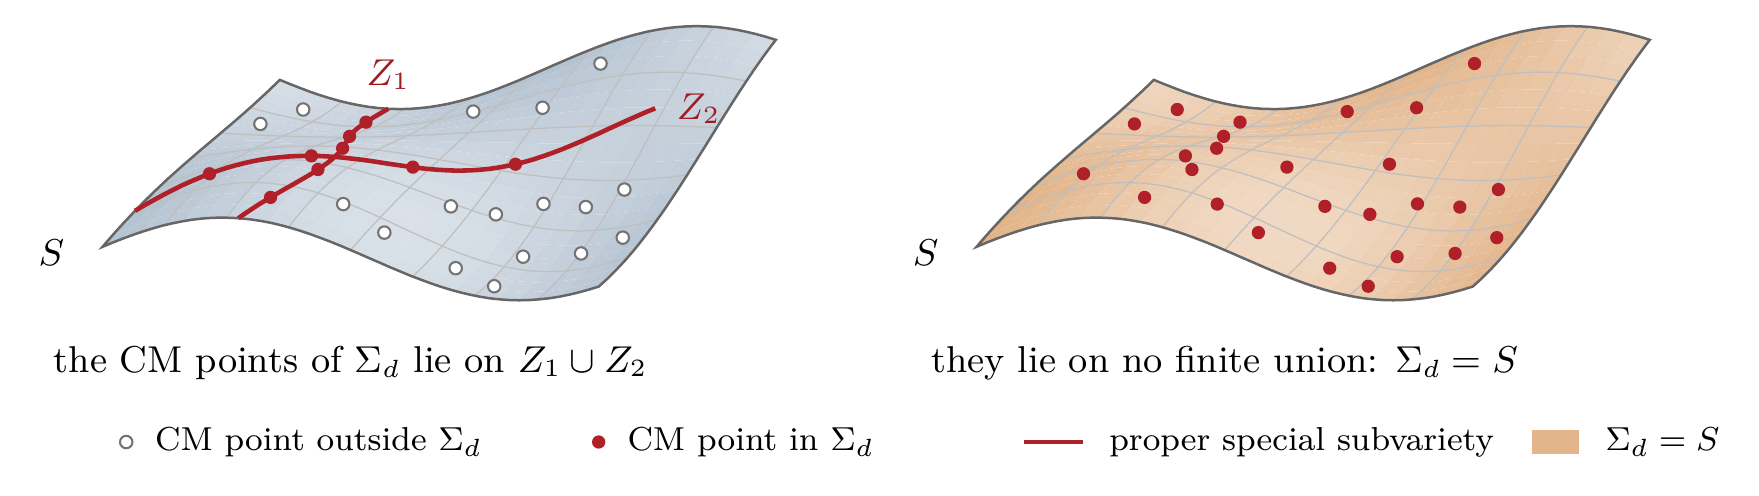
\includegraphics[width=\textwidth]{figures/fig_locus}
\caption{The criterion of \Cref{thm:D}, drawn schematically ($S$ has
dimension $n^{2}$). CM points are dense in $S$. On the left the CM points
of $\Sigma_{d}$ lie on two proper special subvarieties $Z_{1}$ and $Z_{2}$,
and condition (iii) fails for this $d$. On the right they lie on no finite
union of proper special subvarieties; by the Andr\'e--Oort theorem their
Zariski closure is then $S$, and $\Sigma_{d}=S$.}
\label{fig:locus}
\end{figure}

\begin{remark}\label{rem:degrees}
Without any hypothesis $\Sigma$ is dense. It contains the members
$K$-isogenous to $E^{n}\times\bar E^{n}$, which is of split Weil type and
whose Weil classes are polynomials in divisor classes (\Cref{lem:EEbar});
and with every point it contains its Hecke orbit, which is dense. Algebraic representatives move
along isogenies by push-forward and pull-back, and their degree grows with
the degree of the isogeny. \st{CM} adds every CM point, but it gives no bound
on the degrees, and by \Cref{thm:D} a bound on a set of CM points that is
not trapped in finitely many proper Shimura subvarieties is exactly what
remains. Neither \cite{OAI26} nor any other source we know gives such a
bound.
\end{remark}

\section{Weil classes and Schoen's subvariety}\label{sec:weil}

In this section $K$ is an imaginary quadratic field with a fixed embedding
$\chi\colon K\to\CC$ and its conjugate $\bar\chi$. Let $A$ be an abelian
variety of Weil type for $K$ of dimension $2n$ (\Cref{ssec:weilfamilies}) on
which $\cO_{K}$ acts, with a polarization class $\eta$ whose Rosati
involution induces complex conjugation on $K$. Endomorphisms act on
cohomology by pull-back, which makes $V=H^{1}(A,\QQ)$ a $K$-vector space of
dimension $2n$, and
\[
  V_{\CC}=V\otimes_{\QQ}\CC=V_{\chi}\oplus V_{\bar\chi},
\]
where $\alpha\in K$ acts on $V_{\chi}$ by $\chi(\alpha)$ and on
$V_{\bar\chi}$ by $\bar\chi(\alpha)$. Each summand has dimension $2n$ and,
because $A$ is of Weil type, meets $H^{1,0}$ and $H^{0,1}$ in subspaces of
dimension $n$. The Weil plane satisfies
\[
  W(A)\otimes\CC=\textstyle\bigwedge^{2n}V_{\chi}\oplus\bigwedge^{2n}V_{\bar\chi}
  \subseteq H^{2n}(A,\CC)
\]
\cite[\S4]{Del82}, and both lines are of type $(n,n)$. We call $A$
\emph{Weil-algebraic} if every class in $W(A)$ is algebraic. Two facts are
used repeatedly. First, an endomorphism $\alpha\in\cO_{K}$ multiplies
$\eta$ by the norm $N(\alpha)=\chi(\alpha)\bar\chi(\alpha)$, since its Rosati
adjoint is $\bar\alpha$; comparing with the action of $\alpha$ on
$\bigwedge^{2}V_{\CC}=\bigwedge^{2}V_{\chi}\oplus(V_{\chi}\otimes
V_{\bar\chi})\oplus\bigwedge^{2}V_{\bar\chi}$ for any $\alpha\notin\QQ$ shows
that $\eta\in V_{\chi}\otimes V_{\bar\chi}$, and hence
\begin{equation}\label{eq:etapower}
  \eta^{k}\in\textstyle\bigwedge^{k}V_{\chi}\otimes\bigwedge^{k}V_{\bar\chi}.
\end{equation}
Second, if $W(A)$ contains one nonzero algebraic class, then $A$ is
Weil-algebraic, by the argument given for $\xi_{s}$ in
\Cref{ssec:weilfamilies}.

The Hodge group $\Hg(A)$ commutes with $K$ and preserves the Riemann form,
so it lies in the unitary group $\U(V,H)$ of the hermitian form $H$ of the
polarization. It fixes the Hodge classes in $W(A)$, on which $\U(V,H)$ acts
through the determinant, so $\Hg(A)\subseteq\SU(V,H)$. We say that $A$ has
\emph{maximal Hodge group} if equality holds.

\subsection{The Hodge ring of a general member}

\begin{proposition}\label{prop:hodgering}
If $\Hg(A)=\SU(V,H)$, then $\Hdg^{k}(A)=\QQ\,\eta^{k}$ for $k\ne n$, and
\[
  \Hdg^{n}(A)=\QQ\,\eta^{n}\oplus W(A).
\]
Moreover $\eta^{n}\cup w=0$ for every $w\in W(A)$.
\end{proposition}

\begin{proof}
The Hodge classes in $H^{2k}(A,\QQ)=\bigwedge^{2k}V$ are the invariants of
$\Hg(A)$ \cite[\S3]{Del82}. Over $\CC$ the group $\SU(V,H)$ becomes
$\mathrm{SL}(V_{\chi})$, acting on $V_{\chi}$ by the standard representation
and on $V_{\bar\chi}$ by its dual, because the Riemann form pairs
$V_{\bar\chi}$ perfectly with $V_{\chi}$. The invariants in
\[
  \textstyle\bigwedge^{2k}V_{\CC}=\bigoplus_{a+b=2k}\bigwedge^{a}V_{\chi}
  \otimes\bigwedge^{b}V_{\chi}^{\vee}
  =\bigoplus_{a+b=2k}\operatorname{Hom}\bigl(\bigwedge^{b}V_{\chi},
  \bigwedge^{a}V_{\chi}\bigr)
\]
form a line in each summand with $a=b$ or $\{a,b\}=\{0,2n\}$, and vanish in
the others, because the representations $\bigwedge^{a}V_{\chi}$, $0\le
a\le2n$, are irreducible and pairwise non-isomorphic except for
$\bigwedge^{0}\cong\bigwedge^{2n}$.\footnote{The representation
$\bigwedge^{a}$ of $\mathrm{SL}_{2n}$ is irreducible with highest weight the
$a$-th fundamental weight for $1\le a\le 2n-1$, and these weights are
distinct; $\bigwedge^{0}$ and $\bigwedge^{2n}$ are trivial.} By
\eqref{eq:etapower} the line for $a=b=k$ contains $\eta^{k}$, which is
nonzero for $k\le2n$ because $\eta^{2n}$ is a positive multiple of the
orientation class. In degree $2n$ the two remaining lines span
$W(A)\otimes\CC$. This proves the first two assertions. By
\eqref{eq:etapower}, $\eta^{n}\cup\bigwedge^{2n}V_{\chi}$ lies in
$\bigwedge^{3n}V_{\chi}\otimes\bigwedge^{n}V_{\bar\chi}=0$, and likewise for
$V_{\bar\chi}$.
\end{proof}

\subsection{What is known}\label{ssec:weilknown}
For $n=1$ the Weil plane lies in $H^{2}$ and \Cref{thm:lef11} applies. For
$n=2$ the hermitian form is split exactly when its discriminant is trivial,
and Floccari and Fu prove that the Weil classes of every Weil fourfold of
discriminant one are algebraic \cite{FF26}. Schoen proves algebraicity for
the Weil fourfolds of trivial discriminant for $\QQ(\sqrt{-3})$ and for the
Weil sixfolds of a family for $\QQ(\sqrt{-3})$ in which his Prym varieties
are dense \cite{Sch88,Sch98}, and for further families of fourfolds
\cite{Sch98}; Koike treats families for $\QQ(\sqrt{-1})$ built in the same
way \cite{Koi04}. Markman's preprint proves algebraicity for every Weil
fourfold and every split Weil sixfold \cite{Mar25a}. Since the Hodge ring of
an abelian variety of dimension at most five is generated by divisor classes
and the Weil classes of its quotients \cite{MZ99}, the fourfold case gives
\st{F2} in dimension at most five. For $2n\ge8$ we know of
no family of Weil type whose general member has maximal Hodge group and on
which the Weil classes are known to be algebraic at every member.

\subsection{Semiregularity}\label{ssec:semireg}
Let $Z$ be a smooth projective variety of dimension $N$ and $\mathcal{E}$ a
coherent sheaf on $Z$, with Atiyah class
$\operatorname{at}(\mathcal{E})\in\operatorname{Ext}^{1}(\mathcal{E},
\mathcal{E}\otimes\Omega^{1}_{Z})$. The \emph{semiregularity map} of
Buchweitz and Flenner is
\[
  \sigma_{\mathcal{E}}\colon\operatorname{Ext}^{2}(\mathcal{E},\mathcal{E})
  \longrightarrow\bigoplus_{q=0}^{N-2}H^{q+2}(Z,\Omega^{q}_{Z}),\qquad
  e\longmapsto\Bigl(\operatorname{tr}\bigl(\operatorname{at}(\mathcal{E})^{q}
  \circ e\bigr)/q!\Bigr)_{q},
\]
and $\mathcal{E}$ is \emph{semiregular} if $\sigma_{\mathcal{E}}$ is
injective \cite{BF03}. A subvariety $Y\subseteq Z$ is semiregular if
$\cO_{Y}$ is.\footnote{Bloch introduced semiregularity for local complete
intersection subvarieties, through a map $H^{1}(Y,N_{Y/Z})\to
H^{p+1}(Z,\Omega^{p-1}_{Z})$ in codimension $p$, and proved the deformation
theorem below in that setting \cite{Blo72}. Buchweitz and Flenner extend
both the map and the theorem to coherent sheaves.} The point of the
definition is the following theorem. If an infinitesimal deformation of $Z$
keeps $\ch(\mathcal{E})$ of Hodge type, the obstruction to deforming
$\mathcal{E}$ along it is sent by $\sigma_{\mathcal{E}}$ to the obstruction
for $\ch(\mathcal{E})$ to stay of Hodge type, which vanishes; injectivity
of $\sigma_{\mathcal{E}}$ then kills the first obstruction.

\begin{theorem}[{Buchweitz--Flenner \cite[Theorem~1.5]{BF03}, after Bloch
\cite{Blo72}}]\label{thm:bf}
Let $f\colon\mathcal{Z}\to T$ be a smooth projective morphism to a connected
complex manifold, let $0\in T$, and let $\mathcal{E}$ be a semiregular
coherent sheaf on $\mathcal{Z}_{0}$. Suppose that over a contractible
neighbourhood of $0$ the flat continuation of every component of
$\ch(\mathcal{E})$ is a Hodge class on every fibre. Then $\mathcal{E}$
extends to a coherent sheaf on $f^{-1}(U)$, flat over $U$, for some open
neighbourhood $U$ of $0$.
\end{theorem}

We return to the split Weil family $\pi\colon\cA\to S$ of
\Cref{ssec:weilfamilies}, with its global section $\xi$ of Weil planes and
the sets $\Sigma_{d}\subseteq\Sigma\subseteq S$ of \Cref{def:sigmad}.

\begin{proposition}\label{prop:semireg}
Let $s_{0}\in S$ and let $\mathcal{E}$ be a semiregular coherent sheaf on
$A=\cA_{s_{0}}$ such that $\ch_{k}(\mathcal{E})\in\QQ\,\eta^{k}$ for $k\ne
n$ and $\ch_{n}(\mathcal{E})=a\,\eta^{n}+w$ with $a\in\QQ$ and $0\ne w\in
W(A)$. Then $\Sigma=S$: the Weil classes are algebraic on every member of
the family.
\end{proposition}

\begin{proof}
The powers of $\eta$ extend to flat sections that are Hodge classes on every
member, and so does $w$, since the Weil planes form a trivial local system
of Hodge classes on $S$ (\Cref{ssec:weilfamilies}). So the hypothesis of
\Cref{thm:bf} holds, and $\mathcal{E}$ extends to a sheaf on
$\pi^{-1}(U)$, flat over $U$, for a contractible open neighbourhood $U$ of
$s_{0}$ in $S^{\mathrm{an}}$. For $t\in U$ its restriction $\mathcal{E}_{t}$
is algebraic by GAGA and has a finite locally free resolution, so
$\ch(\mathcal{E}_{t})$ is algebraic, and it is the flat continuation of
$\ch(\mathcal{E})$. Hence $w_{t}=\ch_{n}(\mathcal{E}_{t})-a\,\eta_{t}^{n}$ is
a nonzero algebraic class in $W(\cA_{t})$, and $t\in\Sigma$. Thus
$U\subseteq\Sigma=\bigcup_{d}\Sigma_{d}$. By the Baire category theorem some
$\Sigma_{d}$ contains a nonempty open subset of $S^{\mathrm{an}}$; it is
Zariski closed by \Cref{lem:sigmaclosed} and $S$ is irreducible, so
$\Sigma_{d}=S$.
\end{proof}

\subsection{Schoen's subvariety}\label{ssec:schoen}
From now on $K=\QQ(\sqrt{-3})$, and $\zeta\in\cO_{K}$ is a primitive cube
root of unity. Let $X$ be a curve of genus $g=n+1\ge3$, let $L\in
\Pic^{0}(X)$ have exact order three, and let $\pi\colon C\to X$ be the
\'etale cyclic triple cover defined by $L$, with covering automorphism
$\sigma$; thus $\pi_{*}\cO_{C}=\cO_{X}\oplus L\oplus L^{2}$, and $C$ has
genus $3g-2$. In $J=J(C)$ put $N=1+\sigma+\sigma^{2}$ and $P=3-N$, and let
$B=P(J)$, the \emph{Prym variety} of the cover, with the polarization $\eta$
induced by the principal polarization of $J$. Since $N^{2}=3N$, we have
$NP=0$ and $P^{2}=3P$; so $P$ is multiplication by $3$ on $B$, and $\sigma$
acts on $B$ with $\sigma^{2}+\sigma+1=0$, which lets $\zeta$ act as $\sigma$.

\begin{lemma}\label{lem:prym}
\begin{enumerate}[label=\textup{(\alph*)}]
\item $B$ is an abelian variety of Weil type for $K$ of dimension $2n$.
\item The hermitian form of $\eta$ is split.
\item For very general $(X,L)$, $B$ has maximal Hodge group.
\end{enumerate}
\end{lemma}

\begin{proof}
(a) By the decomposition of $\pi_{*}\cO_{C}$, the space $H^{0}(C,K_{C})$ is
the sum of $H^{0}(X,K_{X}\otimes L^{j})$, $j=0,1,2$, on which $\sigma^{*}$
acts by the three cube roots of unity. By Riemann--Roch these spaces have
dimensions $g$, $g-1$ and $g-1$, since $L^{j}$ is a nontrivial bundle of
degree zero for $j=1,2$. Let $P'\colon J\to B$ be $P$ with its target
restricted and $\iota\colon B\to J$ the inclusion. Since $P'\iota=3$ and
$P=\iota P'$, pull-back by $P'$ identifies $H^{1,0}(B)$ with the image of
$P^{*}=3-N^{*}$ on $H^{1,0}(J)$, which is the sum of the two nontrivial
eigenspaces. So $\dim B=2(g-1)=2n$, and both embeddings of $K$ occur with
multiplicity $n$.

(b) The Riemann form of $\eta$ is the intersection form $E$ on
$H_{1}(B,\QQ)=P\,H_{1}(C,\QQ)$, and a $K$-subspace is isotropic for the
hermitian form exactly when it is isotropic for $E$. The cover corresponds to
a surjection $\phi\colon H_{1}(X,\ZZ)\to\ZZ/3$. Since $\mathrm{Sp}_{2g}(\ZZ)$
maps onto $\mathrm{Sp}_{2g}(\ZZ/3)$, which is transitive on nonzero vectors,
there is a symplectic basis $a_{1},b_{1},\dots,a_{g},b_{g}$ with
$\phi(x)=\langle x,b_{1}\rangle\bmod 3$; represent it by simple closed
curves in standard position. For $i\ge2$ the curves $a_{i}$ and $b_{i}$ have
trivial monodromy, so each lifts to three disjoint closed curves, permuted by
$\sigma$. Choose lifts $\tilde a_{i}$ and $\tilde b_{i}$ that meet. Then
$E(\sigma^{k}\tilde a_{i},\sigma^{l}\tilde a_{j})=0$ and
$E(\sigma^{k}\tilde a_{i},\sigma^{l}\tilde b_{j})=\delta_{ij}\delta_{kl}$
for $i,j\ge2$. The first relation shows that the $\ZZ[\sigma]$-span of the
classes $P\tilde a_{i}$, $2\le i\le g$, is isotropic. These classes are
$K$-linearly independent: if $\sum_{i}\alpha_{i}P\tilde a_{i}=0$ with
$\alpha_{i}=\sum_{k}c_{ik}\sigma^{k}\in\ZZ[\sigma]$, pairing with
$\sigma^{l}\tilde b_{j}$ gives $3c_{jl}-\sum_{k}c_{jk}=0$ for every $l$, so
$c_{j0}=c_{j1}=c_{j2}$ and $\alpha_{j}$ is a multiple of $N$, which is zero
on $B$. So they span an isotropic subspace of dimension $n=g-1$.

(c) The monodromy of the Prym varieties over the moduli of pairs $(X,L)$ is
an arithmetic subgroup of the unitary group \cite{Loo97}, so by Borel density its Zariski closure contains
$\SU(V,H)$. By Andr\'e's theorem \cite{And92} the connected
monodromy group is contained in the Hodge group of a very general member.
Together with $\Hg(B)\subseteq\SU(V,H)$ this gives equality.
\end{proof}

The pairs $(X,L)$ of genus $g$ have $3g-3=3n$ moduli, while the split Weil
family of $K$ in dimension $2n$ has dimension $n^{2}$. For $n\le3$ Schoen uses these Prym varieties to reach every member
\cite{Sch88,Sch98}. For $n\ge4$ they form a proper subvariety
(\Cref{fig:dims}).

\begin{figure}[t]
\centering
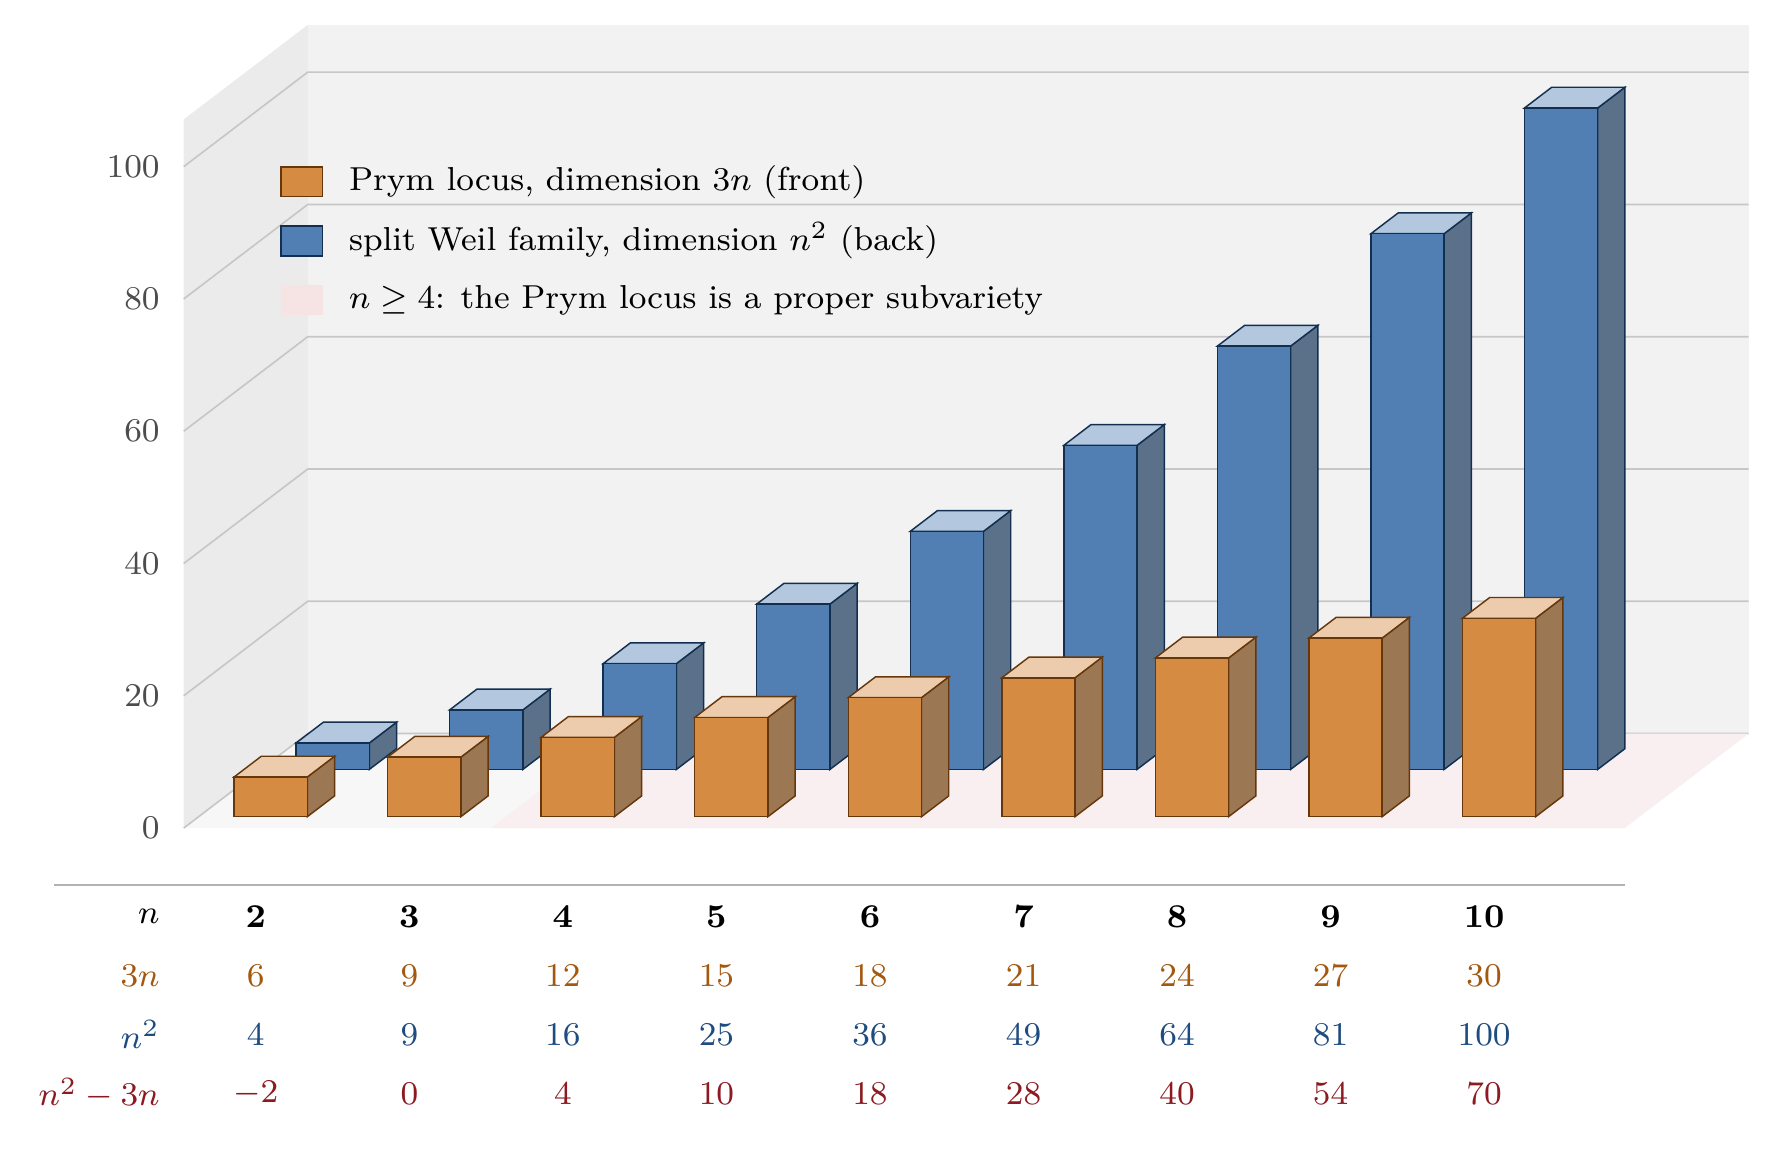
\includegraphics[width=0.9\textwidth]{figures/fig_dims}
\caption{The dimension $3n$ of the locus of Prym varieties of \'etale
cyclic triple covers of curves of genus $n+1$, against the dimension $n^{2}$
of the split Weil family of $\QQ(\sqrt{-3})$ in dimension $2n$. For $n\ge4$
the Prym locus is a proper subvariety, and a semiregular $Y$ would have to
deform in the $n^{2}-3n$ remaining directions.}
\label{fig:dims}
\end{figure}

\emph{The construction.} Let $h=2g-2=2n$. The group
$G=(\ZZ/3)^{h}\rtimes S_{h}$ acts on $C^{h}$ by
$(v,\tau)\cdot(c_{i})_{i}=(\sigma^{v_{i}}c_{\tau^{-1}(i)})_{i}$, and the
quotient is the symmetric product $X^{(h)}$; write $\mu\colon C^{h}\to
X^{(h)}$. The map $\varepsilon(v,\tau)=\sum_{i}v_{i}$ is a homomorphism
$G\to\ZZ/3$, with kernel $G'$. Following Schoen \cite[\S2]{Sch88}, put
\[
  W_{0}=C^{h}/G',\qquad \rho\colon C^{h}\to W_{0},\qquad
  \nu\colon W_{0}\to X^{(h)},
\]
and let $\delta=\sigma\times1\times\dots\times1$, so that $\varepsilon(\delta)
=1$ and $\delta$ induces an automorphism $\bar\delta$ of $W_{0}$ over
$X^{(h)}$.

\begin{lemma}\label{lem:quotient}
\begin{enumerate}[label=\textup{(\alph*)}]
\item No element of $G\setminus G'$ has a fixed point on $C^{h}$. Hence
$\nu$ is a connected \'etale Galois cover with group $\ZZ/3$, generated by
$\bar\delta$.
\item $G$ acts freely on $\mu^{-1}(D)$ for every reduced divisor $D\in
X^{(h)}$.
\item $\mu$ is finite and flat, so $\mu^{-1}$ of a subvariety of pure
dimension $r$ has pure dimension $r$.
\end{enumerate}
\end{lemma}

\begin{proof}
Suppose $(v,\tau)$ fixes $(c_{i})$, so that
$c_{\tau(i)}=\sigma^{v_{\tau(i)}}c_{i}$ for all $i$. Going once around a
cycle $(i_{1},\dots,i_{k})$ of $\tau$ gives $c_{i_{1}}=\sigma^{v_{i_{1}}+
\dots+v_{i_{k}}}c_{i_{1}}$; since $\sigma$ has no fixed points, the sum of
the $v_{i}$ over every cycle is $0$ in $\ZZ/3$, and so is
$\varepsilon(v,\tau)$. This is~(a): $W_{0}$ is connected as a quotient of
$C^{h}$, and $G/G'\cong\ZZ/3$ acts freely on it with quotient $X^{(h)}$. If
moreover the points $\pi(c_{i})$ are distinct, then $\pi(c_{\tau(i)})=
\pi(c_{i})$ forces $\tau=1$, and then $v=0$; this is~(b). The map $C^{h}\to
X^{h}$ is \'etale and $X^{h}\to X^{(h)}$ is a finite map between smooth
varieties of the same dimension, hence flat. By going down for flat maps,
every component of the preimage of a subvariety $Z$ dominates a component of
$Z$, and the fibres are finite; this gives~(c).
\end{proof}

Let $u\colon X^{(h)}\to\Pic^{h}(X)$ send $D$ to $\cO_{X}(D)$. Its fibre over
$[K_{X}]$ is the canonical system $F=|K_{X}|\cong\PP^{n}$. Since $F$ is
simply connected, the restriction of $\nu$ to $\nu^{-1}(F)$ is a trivial
cover: $\nu^{-1}(F)=Q_{0}\sqcup Q_{1}\sqcup Q_{2}$ with each $Q_{t}$ mapped
isomorphically onto $F$, and $\bar\delta$, which has no fixed points,
permutes the $Q_{t}$ cyclically; number them so that
$\bar\delta(Q_{t})=Q_{t+1}$. These are the three components of Schoen's
construction.\footnote{Patel and Zhang obtain the same three components by
base change of the Abel--Jacobi map along an isogeny onto $J(X)$
\cite{PZ25}.} Put
\[
  \Lambda_{0}=\rho^{-1}(Q_{0})\subseteq C^{h},
\]
with its reduced structure. It has pure dimension $n$ by
\Cref{lem:quotient}(c), and since the general member of $|K_{X}|$ is
reduced, $\rho$ is \'etale over a dense open subset of $Q_{0}$ by
\Cref{lem:quotient}(b), so that $\rho_{*}[\Lambda_{0}]=|G'|\,[Q_{0}]$. The construction is drawn in \Cref{fig:schoen}.

\begin{figure}[t]
\centering
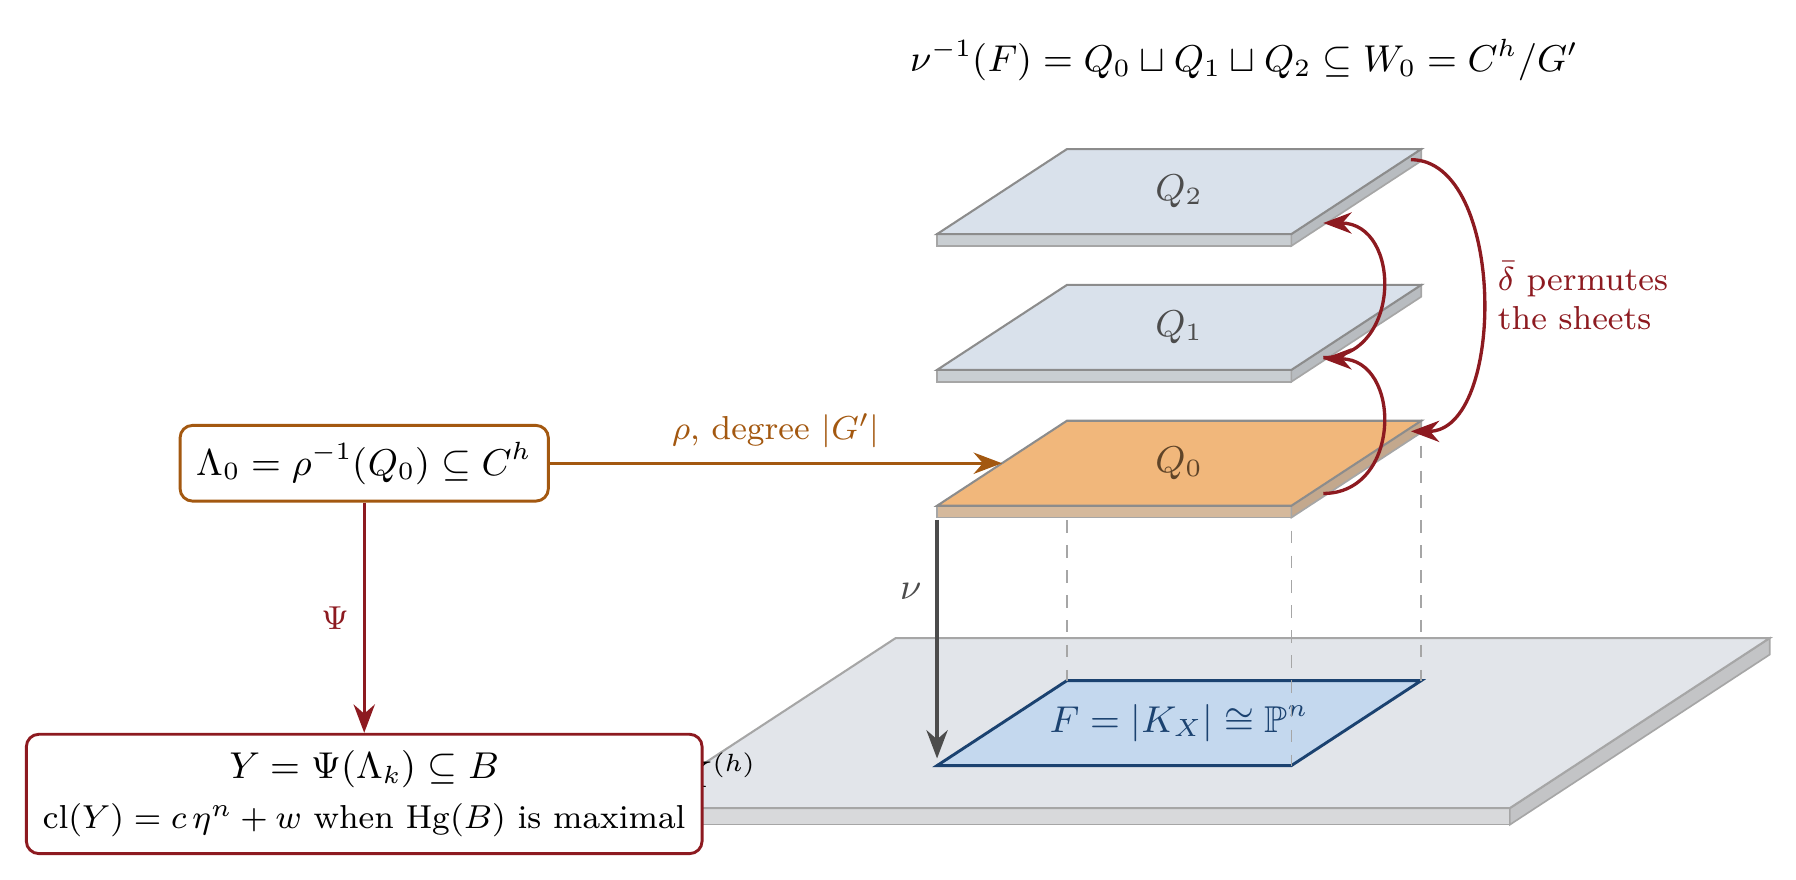
\includegraphics[width=\textwidth]{figures/fig_schoen}
\caption{Schoen's construction. Over the canonical system $F=|K_{X}|$ of
$X$, the \'etale triple cover $\nu\colon W_{0}\to X^{(h)}$ splits into three
sheets, which $\bar\delta$ permutes cyclically. $\Lambda_{0}\subseteq C^{h}$
is the preimage of one sheet, and $Y$ is the image under $\Psi$ of one of
its components (\Cref{thm:E}).}
\label{fig:schoen}
\end{figure}

Fix $c_{0}\in C$ and let
\[
  \Psi\colon C^{h}\to B,\qquad (c_{1},\dots,c_{h})\mapsto
  P\Bigl(\,\sum_{i}(c_{i}-c_{0})\Bigr).
\]

The key input is a computation of cohomology with twisted coefficients.

\begin{lemma}\label{lem:twisted}
Let $\mathcal{L}$ be a nontrivial local system of rank one on $X^{(h)}$.
Then restriction $H^{h}(X^{(h)},\mathcal{L})\to H^{h}(F,\mathcal{L})$ is an
isomorphism, and $H^{h}(F,\mathcal{L})\cong H^{2n}(\PP^{n},\CC)\cong\CC$.
\end{lemma}

\begin{proof}
The fibres of $u$ are projective spaces, so $\mathcal{L}$ is trivial on each
of them, and $\mathcal{M}=u_{*}\mathcal{L}$ is a local system of rank one on
$T=\Pic^{h}(X)$ with $\mathcal{L}=u^{*}\mathcal{M}$.\footnote{By proper base
change the stalk of $u_{*}\mathcal{L}$ at $y$ is $H^{0}(u^{-1}(y),
\mathcal{L})\cong\CC$, so a nonzero section over the fibre extends over
$u^{-1}(D)$ for a small ball $D\ni y$. This set is connected, since $u$ is
proper with connected fibres, and a section of a local system of rank one
over a connected set is determined by its value at one point and vanishes
nowhere unless it is zero. So restriction from $u^{-1}(D)$ to each fibre
over $D$ is an isomorphism, $u_{*}\mathcal{L}$ is locally constant, and
$u^{*}u_{*}\mathcal{L}\to\mathcal{L}$ is an isomorphism on stalks.} It is
nontrivial, because $\mathcal{L}$ is. As a real manifold $T$ is a torus
$(S^{1})^{2g}$, and $\mathcal{M}$ is an exterior product of local systems on
the circles, at least one of them nontrivial; a nontrivial local system of
rank one on a circle has no cohomology, so $H^{*}(T,\mathcal{M})=0$ by the
K\"unneth formula. Let $U=T\setminus\{[K_{X}]\}$. The exact sequence
\[
  \dots\to H^{k}_{c}(U,\mathcal{M})\to H^{k}(T,\mathcal{M})\to
  H^{k}(\{[K_{X}]\},\mathcal{M})\to H^{k+1}_{c}(U,\mathcal{M})\to\dots
\]
gives $H^{1}_{c}(U,\mathcal{M})\cong\CC$ and $H^{k}_{c}(U,\mathcal{M})=0$ for
$k\ne1$. For $M\in U$ Riemann--Roch gives $h^{0}(M)=g-1=n$, so over $U$ the
map $u$ is the projective bundle of a vector bundle of rank $n$
\cite[Chapter~IV]{ACGH85}, and by the Leray--Hirsch theorem
$H^{*}_{c}(u^{-1}(U),\mathcal{L})\cong H^{*}_{c}(U,\mathcal{M})\otimes
H^{*}(\PP^{n-1})$, which vanishes outside the degrees $1,3,\dots,2n-1$. The
exact sequence of the pair $(X^{(h)},F)$,
\[
  H^{h}_{c}(u^{-1}(U),\mathcal{L})\to H^{h}(X^{(h)},\mathcal{L})\to
  H^{h}(F,\mathcal{L})\to H^{h+1}_{c}(u^{-1}(U),\mathcal{L}),
\]
has zero outer terms, since $h=2n$. Finally $\mathcal{L}$ is trivial on the
simply connected $F\cong\PP^{n}$.
\end{proof}

\begin{proof}[Proof of \Cref{thm:E}]
Write $V_{\chi},V_{\bar\chi}\subseteq H^{1}(B,\CC)$ for the eigenspaces of
$\sigma^{*}$ with eigenvalues $\lambda=\chi(\zeta)$ and $\bar\lambda$, and
choose a basis $\bar y_{1},\dots,\bar y_{h}$ of $V_{\bar\chi}$; put
$\bar\omega=\bar y_{1}\wedge\dots\wedge\bar y_{h}$, which spans
$\bigwedge^{2n}V_{\bar\chi}\subseteq W(B)\otimes\CC$.

\emph{Step 1: the pull-back of $\bar\omega$.} Write $\Psi=P'\circ\Xi$, where
$\Xi(c_{1},\dots,c_{h})=\sum_{i}\operatorname{aj}(c_{i})$ and
$\operatorname{aj}(c)=[c-c_{0}]$ is the Abel--Jacobi map. On $H^{1}$ the
pull-back by the addition map $J^{h}\to J$ is the sum of the pull-backs by
the projections, so $\Psi^{*}\bar y_{j}=\sum_{i}p_{i}^{*}\tilde y_{j}$, where
$p_{i}$ is the $i$-th projection of $C^{h}$ and $\tilde y_{j}=
\operatorname{aj}^{*}P'^{*}\bar y_{j}\in H^{1}(C,\CC)$. Since $P'^{*}$ is
injective and $\operatorname{aj}^{*}$ is an isomorphism, both commuting with
$\sigma^{*}$, the $\tilde y_{j}$ are independent and lie in the
$\bar\lambda$-eigenspace of $\sigma^{*}$ on $H^{1}(C,\CC)$. That eigenspace
has dimension $h$, because the invariant part of $H^{1}(C,\CC)$ is
$\pi^{*}H^{1}(X,\CC)$, of dimension $2g$, and the two other eigenspaces are
conjugate; so the $\tilde y_{j}$ form a basis of it. Now
\[
  u:=\Psi^{*}\bar\omega=\prod_{j=1}^{h}\Bigl(\sum_{i=1}^{h}p_{i}^{*}
  \tilde y_{j}\Bigr).
\]
A product $\tilde y_{j}\cup\tilde y_{k}$ lies in the
$\bar\lambda^{2}$-eigenspace of $H^{2}(C,\CC)$, which is zero because
$\sigma$ acts trivially on $H^{2}(C)$ and $\bar\lambda^{2}\ne1$. So in the
expansion only the terms with one factor on each $p_{i}$ survive:
$u=\sum_{s\in S_{h}}\pm\prod_{i}p_{i}^{*}\tilde y_{s(i)}$. By the K\"unneth
formula these terms are linearly independent, and $u\ne0$. Each term is
multiplied by $\bar\lambda^{\sum v_{i}}$ under $(\sigma^{v_{1}}\times\dots
\times\sigma^{v_{h}})^{*}$, and $u$ is symmetric because $\Psi$ is; so $u$
is invariant under $G'$, and $\delta^{*}u=\bar\lambda u$.

\emph{Step 2: restriction to $Q_{0}$.} By transfer, $\rho^{*}$ identifies
$H^{*}(W_{0},\CC)$ with $H^{*}(C^{h},\CC)^{G'}$, so $u=\rho^{*}\bar u$ for a
class $\bar u\ne0$ with $\bar\delta^{*}\bar u=\bar\lambda\bar u$. The
decomposition $\nu_{*}\CC=\bigoplus_{\psi}\mathcal{L}_{\psi}$ into
eigensheaves of $\bar\delta$, indexed by the characters $\psi$ of $\ZZ/3$,
identifies the $\psi(1)$-eigenspace of $\bar\delta^{*}$ on
$H^{*}(W_{0},\CC)$ with $H^{*}(X^{(h)},\mathcal{L}_{\psi})$, compatibly with
restriction to $\nu^{-1}(F)$ and $F$. For $\psi\ne1$ the local system
$\mathcal{L}_{\psi}$ is nontrivial, since $H^{0}(W_{0},\CC)$ is the
invariant line. By \Cref{lem:twisted}, $\bar u$ restricts to a nonzero class
on $\nu^{-1}(F)=Q_{0}\sqcup Q_{1}\sqcup Q_{2}$. As $\bar\delta$ maps $Q_{0}$
isomorphically onto $Q_{t}$ and $\bar u$ is an eigenvector, $\bar u|_{Q_{0}}
=0$ would force $\bar u|_{Q_{t}}=0$ for every $t$. Hence
$\int_{Q_{0}}\bar u\ne0$, and
\[
  \int_{B}\Psi_{*}[\Lambda_{0}]\cup\bar\omega
  =\int_{[\Lambda_{0}]}\rho^{*}\bar u
  =|G'|\int_{Q_{0}}\bar u\ne0.
\]

\emph{Step 3: one component.} The class $\Psi_{*}[\Lambda_{0}]$ is
$\sum_{k}e_{k}\cl(\Psi(\Lambda_{k}))$, the sum over the irreducible
components $\Lambda_{k}$ of $\Lambda_{0}$ on which $\Psi$ is generically
finite, with $e_{k}$ the degree of $\Lambda_{k}\to\Psi(\Lambda_{k})$. By Step
2 one of them, say $Y=\Psi(\Lambda_{k})$, satisfies $\int_{B}\cl(Y)\cup
\bar\omega\ne0$. It is irreducible of dimension $n$. Since $W(B)\otimes\CC$
is spanned by $\bar\omega$ and its conjugate, $\cl(Y)$ pairs nontrivially
with $W(B)$.

\emph{Step 4: the shape of the class.} If $\Hg(B)=\SU(V,H)$, then
\Cref{prop:hodgering} gives $\cl(Y)=c\,\eta^{n}+w$ with $c\in\QQ$ and $w\in
W(B)$. Since $\eta^{n}\cup\bar\omega=0$, Step~3 gives $w\ne0$. Since
$\eta^{n}\cup w=0$,
\[
  c\int_{B}\eta^{2n}=\int_{B}\cl(Y)\cup\eta^{n}=\deg_{\eta}Y>0,
\]
so $c>0$. The last assertion of \Cref{thm:E} is \Cref{cor:schoensemireg}
below.
\end{proof}

\begin{corollary}[Schoen \cite{Sch88}]\label{cor:schoen}
For every \'etale cyclic triple cover of a curve of genus at least three,
the Prym variety $B$ is Weil-algebraic.
\end{corollary}

\begin{proof}
If $B$ has maximal Hodge group, $w=\cl(Y)-c\,\eta^{n}$ is a nonzero
algebraic class in $W(B)$, and $B$ is Weil-algebraic. By
\Cref{lem:prym}(c) this covers every $(X,L)$ outside a countable union of
proper closed subsets $Z_{i}$ of a smooth connected base $T$ over which, after a finite \'etale
base change, the Prym varieties form a polarized abelian scheme with a
trivial local system of Weil planes.\footnote{Take for $T$ a connected
component of a finite \'etale cover of the moduli space of curves of genus
$g$ with level-$3$ structure, on which $L$ is the section given by a fixed
nonzero vector of $(\ZZ/3)^{2g}$. The monodromy acts on the Weil planes
through the determinant, which takes values in the roots of unity of
$\cO_{K}$, so it becomes trivial on a finite cover.} The proof of
\Cref{lem:sigmaclosed} shows that the locus where the Weil classes have
algebraic representatives of degree at most $d$ is Zariski closed in $T$.
These countably many closed sets, together with the $Z_{i}$, cover $T$, so
by the Baire category theorem one of them has interior. It is not a $Z_{i}$,
so it is one of the degree-$d$ loci, and it equals $T$.
\end{proof}

\begin{corollary}\label{cor:schoensemireg}
Suppose that for one $(X,L)$ of genus $n+1\ge3$ with maximal Hodge group the
subvariety $Y$ of \Cref{thm:E} is semiregular. Then every abelian variety of
split Weil type for $\QQ(\sqrt{-3})$ of dimension $2n$ is Weil-algebraic.
\end{corollary}

\begin{proof}
The sheaf $\cO_{Y}$ has $\ch_{k}(\cO_{Y})=0$ for $k<n$ and $\ch_{n}(\cO_{Y})=
\cl(Y)=c\,\eta^{n}+w$ with $w\ne0$ \cite[Chapter~15]{Ful98}; for $k>n$ the
class $\ch_{k}(\cO_{Y})$ is algebraic, hence a multiple of $\eta^{k}$ by
\Cref{prop:hodgering}. By \Cref{lem:prym}(b), $B$ is a member of a split
Weil family $S$ as in \Cref{ssec:weilfamilies}, and \Cref{prop:semireg}
gives $\Sigma=S$. Every abelian variety of split Weil type for $K$ of
dimension $2n$ is $K$-isogenous to a member of $S$,\footnote{Two split
hermitian forms of the same dimension are isometric, being orthogonal sums
of hyperbolic planes. An isometry carries the complex structure of the
first variety to a point of the symmetric domain of the second form, and
the two lattices are commensurable in the same $K$-vector space.} and a
$K$-isogeny $f$ carries Weil planes to Weil planes and algebraic classes to
algebraic classes in both directions, through $f^{*}$ and
$(\deg f)^{-1}f_{*}$.
\end{proof}

\subsection{Transfer by correspondences}\label{ssec:transfer}
Schoen's cycles reach a family of dimension $3n$ inside one of dimension
$n^{2}$. One way to spread them is to carry the Weil classes to other
varieties by correspondences. This gives a theorem, but a count of
dimensions shows that it cannot reach the general member by itself.

\begin{lemma}\label{lem:twothree}
Let $B$, $A_{1}$ and $A_{2}$ be of Weil type for $K$, of dimensions
$2(m_{1}+m_{2})$, $2m_{1}$ and $2m_{2}$, and let $f\colon B\to A_{1}\times
A_{2}$ be an isogeny that commutes with $\cO_{K}$.
\begin{enumerate}[label=\textup{(\alph*)}]
\item $f^{*}$ carries a plane in $W(A_{1})\otimes W(A_{2})$ onto $W(B)$;
over $\CC$ the plane is spanned by $\omega_{1}\otimes\omega_{2}$ and
$\bar\omega_{1}\otimes\bar\omega_{2}$, where $\omega_{i}$ spans
$\bigwedge^{2m_{i}}V_{\chi}(A_{i})$.
\item If two of $B$, $A_{1}$, $A_{2}$ are Weil-algebraic, so is the third.
\end{enumerate}
\end{lemma}

\begin{proof}
As in the proof of \Cref{cor:schoensemireg}, we may take $B=A_{1}\times
A_{2}$. Then $V_{\chi}(B)=V_{\chi}(A_{1})\oplus V_{\chi}(A_{2})$, and the top
exterior power of a sum is the tensor product of the top exterior powers;
this is~(a). If $A_{1}$ and $A_{2}$ are Weil-algebraic, every class in
$W(A_{1})\otimes W(A_{2})$ is a sum of products $\pr_{1}^{*}\alpha_{1}\cup
\pr_{2}^{*}\alpha_{2}$ of algebraic classes, so $B$ is Weil-algebraic by~(a).
Suppose that $B$ and $A_{2}$ are Weil-algebraic. On $A_{2}$ we have
$\omega_{2}\cup\omega_{2}=0$, since $\bigwedge^{4m_{2}}V_{\chi}(A_{2})=0$,
while $p=\int\omega_{2}\cup\bar\omega_{2}\ne0$, since
$\bigwedge^{2m_{2}}V_{\chi}\otimes\bigwedge^{2m_{2}}V_{\bar\chi}$ is the top
exterior power of $H^{1}(A_{2},\CC)$; and $p$ is real, because classes of
even degree commute. Nonzero rational classes $x\in W(B)$ and $\gamma\in
W(A_{2})$ have the form $x=s\,\omega_{1}\otimes\omega_{2}+\bar s\,
\bar\omega_{1}\otimes\bar\omega_{2}$ and $\gamma=t\,\omega_{2}+\bar t\,
\bar\omega_{2}$ with $s,t\ne0$. The class
\[
  \pr_{1*}\bigl(x\cup\pr_{2}^{*}\gamma\bigr)=p\,\bigl(s\bar t\,\omega_{1}+
  \bar st\,\bar\omega_{1}\bigr)
\]
is rational, algebraic, nonzero, and lies in $W(A_{1})$.
\end{proof}

\begin{lemma}\label{lem:EEbar}
Let $K$ be any imaginary quadratic field, $E$ an elliptic curve with complex
multiplication by $\cO_{K}$, and $\bar E$ the same curve with $\cO_{K}$
acting through complex conjugation. For $k\ge1$ the variety $E^{k}\times
\bar E^{k}$, with the product polarization, is of split Weil type, and its
Weil classes are polynomials in divisor classes.
\end{lemma}

\begin{proof}
On $H_{1}(E,\QQ)=K$ the polarization is $\operatorname{Tr}_{K/\QQ}(f\,x\bar
y)$ for some $f\in K$ with $\bar f=-f$, so its hermitian form is
$x\bar y$. For $\bar E$ the $K$-structure is conjugated, and the same
Riemann form is $\operatorname{Tr}_{K/\QQ}(f\cdot(-\bar xy))$, with
hermitian form $-\bar xy$. So the form of $E^{k}\times\bar E^{k}$ is
$\operatorname{diag}(1,\dots,1,-1,\dots,-1)$, for which the vectors
$e_{i}+e_{k+i}$ span an isotropic subspace of dimension $k$, and both
embeddings of $K$ occur $k$ times on $H^{1,0}$. With coordinates
$z_{1},\dots,z_{2k}$ on the factors, $V_{\chi}$ is spanned by $dz_{1},\dots,
dz_{k}$ and $d\bar z_{k+1},\dots,d\bar z_{2k}$, so up to sign
$\omega_{\chi}=\bigwedge_{i=1}^{k}(dz_{i}\wedge d\bar z_{k+i})$. Each factor
is a class of type $(1,1)$ on $E\times\bar E\cong E\times E$, whose
N\'eron--Severi group has rank $4=h^{1,1}$ because $E$ has complex
multiplication; so it is a complex combination of divisor classes, and so
are $\omega_{\chi}$ and its conjugate.
\end{proof}

\begin{theorem}\label{thm:transfer}
Let $A$ be an abelian variety of Weil type for $K=\QQ(\sqrt{-3})$, of
dimension $2m\ge2$, on which $\cO_{K}$ acts. There are a smooth curve
$C\subseteq A$, stable under $\zeta$ and with $\zeta$ acting freely on it, so
that $C\to X=C/\zeta$ is an \'etale cyclic triple cover of a curve of some
genus $g\ge m+1$; an abelian variety $A'$ of Weil type of dimension
$2(g-1-m)$; and an isogeny commuting with $\cO_{K}$ between the Prym variety
of $C\to X$ and $A\times A'$. For every such curve, $A$ is Weil-algebraic if
and only if $A'$ is.
\end{theorem}

\begin{proof}
\emph{The curve.} The automorphism $\zeta$ has finitely many fixed points,
the kernel of the isogeny $1-\zeta$. Let $\mathcal{N}$ be ample on $A$. The bundle $\mathcal{N}'=\mathcal{N}\otimes\zeta^{*}\mathcal{N}\otimes
\zeta^{2*}\mathcal{N}$ is isomorphic to its pull-back by $\zeta$, so it carries a linearization for the
cyclic group generated by $\zeta$;\footnote{Choose an isomorphism
$\phi\colon\zeta^{*}\mathcal{N}'\to\mathcal{N}'$. The composite of $\phi$,
$\zeta^{*}\phi$ and $\zeta^{2*}\phi$ is an automorphism of $\mathcal{N}'$,
hence a scalar $c$, and $c^{-1/3}\phi$ is a linearization.} its cube
descends to an ample line bundle $\bar{\mathcal{M}}$ on the normal quotient
$q\colon A\to A/\zeta$, since the stabilizers, of order dividing three, act
trivially on its fibres. For $k$ large, $2m-1$ general members $D_{i}$ of
$|\bar{\mathcal{M}}^{k}|$ meet in a smooth irreducible curve $X$ that avoids
the images of the fixed points, by Bertini's theorem. Then $C=q^{-1}(X)$ is
\'etale over $X$, hence smooth, and it is the complete intersection of the
ample divisors $q^{*}D_{i}$, hence connected. Schoen observes the existence
of such curves in \cite[\S3]{Sch88}.

\emph{The surjection.} By the Lefschetz hyperplane theorem, restriction
$H^{1}(A,\QQ)\to H^{1}(C,\QQ)$ is injective, so the homomorphism
$\alpha\colon J(C)\to A$ induced by the inclusion is surjective; it commutes
with $\zeta$. Since $1+\zeta+\zeta^{2}=0$ in $\cO_{K}$, $\alpha N=0$ and
$\alpha P=3\alpha$. So $\alpha$ maps the Prym variety $B=P(J(C))$ onto $A$,
and $g-1\ge m$.

\emph{The complement.} Let $A'$ be the connected component of the kernel of
$\alpha|_{B}$ and $A''$ its complement in $B$ for the induced polarization.
Both are stable under $\sigma$, which preserves the polarization, so
$\cO_{K}$ acts on them, and $A''\to A$ and $A'\times A''\to B$ are isogenies
commuting with $\cO_{K}$. By \Cref{lem:prym}(a) both embeddings of $K$ occur
$g-1$ times on $H^{1,0}(B)$, and they occur $m$ times on $H^{1,0}(A)$; so
they occur $g-1-m$ times on $H^{1,0}(A')$, and $A'$ is of Weil type.

\emph{The equivalence.} $B$ is Weil-algebraic by \Cref{cor:schoen}, and
\Cref{lem:twothree}(b) gives the equivalence.
\end{proof}

\begin{corollary}\label{cor:transfer}
$A$ is Weil-algebraic as soon as, for one curve as in \Cref{thm:transfer},
the complement $A'$ is $K$-isogenous to a product of Weil-algebraic
varieties, such as Prym varieties of \'etale cyclic triple covers
(\Cref{cor:schoen}), abelian surfaces of Weil type (\Cref{thm:lef11}), and
the varieties $E^{k}\times\bar E^{k}$ (\Cref{lem:EEbar}).
\end{corollary}

\begin{proof}
Products of Weil-algebraic varieties are Weil-algebraic by
\Cref{lem:twothree}(b), and \Cref{thm:transfer} applies.
\end{proof}

When $g-1=m$ the complement is zero and $A$ is $K$-isogenous to a Prym
variety. For larger $g$ the theorem trades the Weil classes of $A$ for those
of $A'$, and since curves of higher degree give complements of every size,
one might hope to choose the curve so that $A'$ is of a known kind. The
count below says that for $m\ge4$ this hope fails at the general member
unless an unexpected intersection occurs.

\begin{remark}\label{rem:count}
Pryms of \'etale triple covers of curves of genus $m+k+1$ form a family of
dimension $3(m+k)$ inside the Weil family of dimension $(m+k)^{2}$. The
varieties $K$-isogenous to $A\times A'$, with $A$ in the family of dimension
$m^{2}$ and $A'$ in a family of dimension $f$, form a subvariety of dimension
$m^{2}+f$. For $A$ to be general the two must meet in dimension at least
$m^{2}$, which needs $3(m+k)+f\ge(m+k)^{2}$ unless they meet in excess
dimension. Products of the varieties of \Cref{cor:transfer} of total
dimension $2k$ have at most $3k$ moduli, and $3(m+k)+3k<(m+k)^{2}$ for every
$k\ge0$ once $m\ge4$. For $m=3$ only $k=0$ passes, the Prym locus itself, and
for $m=2$ exactly $k\le2$ pass. So \Cref{cor:transfer} reaches only a meagre
part of the family once $m\ge4$, unless the Prym locus meets these product
loci in excess dimension, as Schoen anticipated \cite[\S3]{Sch88}. This is a
count, not a proof that no such intersection exists.
\end{remark}

\subsection{Where it stops}\label{ssec:whereitstops}
Everything on the Weil route now rests on one question.

\begin{question}\label{q:schoen}
Let $n\ge4$ and let $(X,L)$ be very general of genus $n+1$. Is the subvariety
$Y\subseteq B$ of \Cref{thm:E} semiregular?
\end{question}

A positive answer forces $Y$ to deform with $B$ to first order along all
$n^{2}$ directions of the Weil family, and not only along the $3n$
directions of the Prym locus; so it asks for $n^{2}-3n$ unexpected first
order deformations. We have not been able to decide the question, and the
closest analogue points the other way.

The Abel--Jacobi curve $C\subseteq J(C)$ of a curve of genus $g\ge4$ is
built from the same map as $Y$. Its class $\theta^{g-1}/(g-1)!$ is a Hodge
class on every principally polarized abelian variety. Yet by the criterion
of Matsusaka and Ran \cite{Mat59,Ran81} a curve with this class exists only
on Jacobians and products of Jacobians, which form a proper subvariety of the
moduli space $\mathcal{A}_{g}$. So the curve does not deform in the
directions normal to the Jacobian locus, and by \Cref{thm:bf} it is not
semiregular. The number of those directions is classical. The tangent space
to $\mathcal{A}_{g}$ at $J(C)$ is dual to $\operatorname{Sym}^{2}H^{0}(K_{C})$,
the tangent space to the Jacobian locus is dual to $H^{0}(2K_{C})$, and by
Max Noether's theorem the multiplication map between them is surjective for
non-hyperelliptic $C$, with kernel the space $I_{2}$ of quadrics containing
the canonical curve. So the Jacobian locus has codimension
\[
  \dim I_{2}=\binom{g+1}{2}-(3g-3)=\frac{(g-2)(g-3)}{2}
\]
at $J(C)$. Schoen's subvariety is the analogue one step up, built from the
fibre of the Abel--Jacobi map over the canonical class, and the
corresponding codimension, that of the Prym locus in the Weil family, is
$n^{2}-3n$. Nothing in the construction of $Y$ moves it off the Prym locus.
This is an analogy and not a proof.

Nor can a branched cover take the place of the \'etale one, because
branching does not enlarge the Prym locus enough.

\begin{proposition}\label{prop:branched}
Let $\pi\colon C\to X$ be a cyclic triple cover of a curve of genus $q$,
branched at $r$ points, with covering automorphism $\sigma$, and let its
Prym variety, the image of $3-N$ on $J(C)$ with $N=1+\sigma+\sigma^{2}$,
have dimension $2n$. Then $2q+r=2n+2$, and the covers with these
invariants form finitely many families, each of dimension $q+2n-1\le3n$,
with equality only for \'etale covers of curves of genus $n+1$. In
particular, for $n\ge4$ a very general member of the split Weil family of
$K$ in dimension $2n$ is not $K$-isogenous to the Prym variety of any cyclic
triple cover, \'etale or branched.
\end{proposition}

\begin{proof}
Since $3$ is prime, every branch point is totally ramified, and the
Riemann--Hurwitz formula $2g(C)-2=3(2q-2)+2r$ gives $g(C)=3q-2+r$. The
invariant part of $H^{0}(C,K_{C})$ under $\sigma^{*}$ is
$\pi^{*}H^{0}(X,K_{X})$, of dimension $q$, and as in the proof of
\Cref{lem:prym}(a) the space $H^{1,0}$ of the Prym variety is the sum of the
two other eigenspaces. So the Prym variety has dimension $g(C)-q=2q-2+r$,
and $2q+r=2n+2$. Given $X$ and the $r$ branch points, the cover corresponds
to a surjection from the fundamental group of the punctured curve onto
$\ZZ/3$, and there are finitely many of these. So the covers form finitely
many families, of dimension $3q-3+r$ when $q\ge2$, $r$ when $q=1$, and
$r-3$ when $q=0$; by $r=2n+2-2q$ each of these equals $q+2n-1$. As $r\ge0$,
$q\le n+1$, so the dimension is at most $3n$, and it equals $3n$ exactly
when $q=n+1$ and $r=0$.

The Prym varieties of each family form the image of a variety of
dimension at most $3n$ in the moduli space, and the $K$-isogenies of a given
degree carry it to finitely many subvarieties of at most the same
dimension. The members of the split
Weil family that are $K$-isogenous to such a Prym variety therefore lie in a
countable union of subvarieties of dimension at most $3n$, which for
$n\ge4$ is less than $n^{2}$.
\end{proof}

The analogy with the Abel--Jacobi curve can be tested on $B$ itself, in
dimension one. Following Lange and Ortega \cite{LO11}, call
\[
  \psi\colon C\to B,\qquad \psi(c)=(1-\sigma)(c-c_{0}),
\]
the \emph{Abel--Prym map}. As $P=(1-\sigma)(1-\sigma^{2})$, the restriction
of $\Psi$ to one factor is $(1-\sigma^{2})\circ\psi$, and $1-\sigma^{2}$ is
an isogeny of $B$. Put $V_{j}=H^{0}(X,K_{X}\otimes L^{j})$, so that
$H^{0}(C,K_{C})=V_{0}\oplus V_{1}\oplus V_{2}$ as in the proof of
\Cref{lem:prym}(a), and let
\[
  \mu_{L}\colon V_{1}\otimes V_{2}\longrightarrow H^{0}(X,K_{X}^{\otimes2})
\]
be multiplication of sections, through an isomorphism $L^{3}\cong\cO_{X}$.
A first-order deformation of $X$ with Kodaira--Spencer class $u\in
H^{1}(X,T_{X})$ carries the \'etale cover along with it, uniquely, and with
it $J(C)$, $\sigma$ and $B$. Write $d\mathcal{P}(u)\in H^{1}(B,T_{B})$ for the
Kodaira--Spencer class of the resulting deformation of $B$. Lange and Ortega
identify the dual of $d\mathcal{P}$ with a multiplication map
\cite{LO11}, and we derive the form of this that we need in the proof
below.

\begin{proposition}\label{prop:abelprym}
Let $v\in H^{1}(B,T_{B})$ be the Kodaira--Spencer class of a first-order
deformation $\mathcal{B}$ of $B$ to which $\sigma$ extends. Then $\psi$
extends to a morphism into $\mathcal{B}$ from some first-order deformation of
$C$ if and only if $v$ lies in the image of $d\mathcal{P}$, and this image has
dimension $\operatorname{rk}\mu_{L}\le3n$. Suppose moreover that $n\ge4$,
that $B$ has maximal Hodge group, and that $S$ is a split Weil family
containing $B$ (\Cref{lem:prym}(b)). Then the tangent vectors to $S$ at $B$ along which
$\psi$ extends form a subspace of codimension at least $n^{2}-3n$, although
$\psi_{*}[C]$ is a rational multiple of $\eta^{2n-1}$, whose flat continuation
is algebraic on every member of $S$.
\end{proposition}

\begin{proof}
All deformations are over $\operatorname{Spec}\CC[t]/(t^{2})$. Suppose that
$\psi$ extends to $\psi_{t}\colon\mathcal{C}\to\mathcal{B}$, where
$\mathcal{C}$ is a deformation of $C$ with class $w\in H^{1}(C,T_{C})$. Cover
$C$ and $B$ by affine open sets $U_{i}$ and $W_{i}$ with $\psi(U_{i})\subseteq
W_{i}$ over which $\mathcal{C}$ and $\mathcal{B}$ are trivial, with
transition automorphisms $1+t\theta_{ij}$ and $1+t\xi_{ij}$, where
$(\theta_{ij})$ and $(\xi_{ij})$ are cocycles of vector fields representing
$w$ and $v$. On $U_{i}$ the map $\psi_{t}$ is $\psi+ts_{i}$ for a section
$s_{i}$ of $\psi^{*}T_{B}$, and compatibility on $U_{i}\cap U_{j}$ reads
$s_{j}-s_{i}=\psi^{*}\xi_{ij}-d\psi(\theta_{ij})$ \cite{Hor74}. Hence
\begin{equation}\label{eq:horikawa}
  \psi^{*}v=H^{1}(d\psi)(w)\quad\text{in }H^{1}(C,\psi^{*}T_{B}),
\end{equation}
where $d\psi\colon T_{C}\to\psi^{*}T_{B}$ is the differential.

We compute both sides by Serre duality. The bundle $T_{B}$ is trivial with
fibre $T_{0}B$, and $\psi^{*}$ identifies $H^{0}(B,\Omega^{1}_{B})$ with
$V_{-}=V_{1}\oplus V_{2}$. Indeed, since $(1-\sigma)N=0$, the pull-back by
$1-\sigma\colon J\to B$ maps $H^{1,0}(B)$ injectively into the sum of the
nontrivial eigenspaces of $\sigma^{*}$ on $H^{1,0}(J)$, which has dimension
$2n=\dim B$, and the Abel--Jacobi map identifies this sum with $V_{-}$. So $H^{1}(C,\psi^{*}T_{B})=H^{1}(C,\cO_{C})\otimes T_{0}B$ is
dual to $H^{0}(C,K_{C})\otimes V_{-}$, and $H^{1}(C,T_{C})$ is dual to
$H^{0}(C,K_{C}^{\otimes2})$. The dual of $d\psi$ is evaluation
$\cO_{C}\otimes V_{-}\to K_{C}$, so the dual of $H^{1}(d\psi)$ is
multiplication
\[
  m\colon H^{0}(C,K_{C})\otimes V_{-}\longrightarrow
  H^{0}(C,K_{C}^{\otimes2})
\]
\cite{LO11}. Thus \eqref{eq:horikawa} says that $\psi^{*}v$, as a
linear form on $H^{0}(C,K_{C})\otimes V_{-}$, is $w\circ m$.

Now use $\sigma$. We have $\psi\sigma=t_{a}\sigma\psi$, where $t_{a}$ is the
translation by $a=(1-\sigma)(\sigma c_{0}-c_{0})$. Translations act trivially
on $H^{1}(B,\cO_{B})$ and on $T_{0}B$, so $\psi^{*}$ commutes with the actions
of $\sigma$, and $m$ is equivariant. As $\sigma$ extends to $\mathcal{B}$, the
class $v$ is invariant, and so is the form $\psi^{*}v$; an invariant form
vanishes on every eigenspace of $\sigma$ with an eigenvalue other than $1$.
The automorphism $\sigma^{*}$ acts on $V_{j}$ by $\kappa^{j}$ for a primitive
cube root of unity $\kappa$, so the invariant part of
$H^{0}(C,K_{C})\otimes V_{-}$ is $E=(V_{1}\otimes V_{2})\oplus(V_{2}\otimes
V_{1})$. Since $\pi_{*}K_{C}^{\otimes2}=K_{X}^{\otimes2}\otimes\pi_{*}\cO_{C}$,
the map $m$ sends $E$ to $H^{0}(C,K_{C}^{\otimes2})^{\sigma}=\pi^{*}H^{0}(X,
K_{X}^{\otimes2})$, by $(x,y)\mapsto\pi^{*}M(x,y)$ with
$M(x,y)=\mu_{L}(x+\tau y)$, where $\tau\colon V_{2}\otimes V_{1}\to
V_{1}\otimes V_{2}$ is the transposition. So $\psi^{*}v$ is determined by its
restriction to $E$, which by \eqref{eq:horikawa} is $f\circ M$, where $f$ is
the linear form $q\mapsto\langle w,\pi^{*}q\rangle$ on
$H^{0}(X,K_{X}^{\otimes2})$, that is, an element of $H^{1}(X,T_{X})$.

Apply this to the deformation of $B$ induced by $u\in H^{1}(X,T_{X})$. The
deformation of $C$ has class $\pi^{*}u$, and $\psi$ extends after $c_{0}$ is
extended to a section. Since $\pi$ has degree $3$, $\langle\pi^{*}u,
\pi^{*}q\rangle=3\langle u,q\rangle$, so the restriction of
$\psi^{*}d\mathcal{P}(u)$ to $E$ is $3\,u\circ M$. Returning to $v$, the
invariant forms $\psi^{*}v$ and $\psi^{*}d\mathcal{P}(f/3)$ agree on $E$,
hence everywhere. The map $\psi^{*}$ on $H^{1}(B,T_{B})=H^{1}(B,\cO_{B})
\otimes T_{0}B$ is injective, since on $H^{1}(B,\cO_{B})$ it is the complex
conjugate of the injective map on $H^{0}(B,\Omega^{1}_{B})$. So
$v=d\mathcal{P}(f/3)$. Conversely, if $v=d\mathcal{P}(u)$, then $\mathcal{B}$
is isomorphic to the deformation induced by $u$, since first-order
deformations are determined by their Kodaira--Spencer classes, and $\psi$
extends. Finally $d\mathcal{P}(u)=0$ exactly when $u\circ M=0$, that is, when
$u$ vanishes on the image of $\mu_{L}$; so $d\mathcal{P}$ has rank
$\operatorname{rk}\mu_{L}\le h^{0}(X,K_{X}^{\otimes2})=3g-3=3n$.

For the last assertion, the element $\zeta\in\cO_{K}$ acts on the abelian
scheme over $S$ as $\sigma$ on $B$, so the Kodaira--Spencer map
$T_{S,B}\to H^{1}(B,T_{B})$ has invariant image. It is injective, because $S$
is locally isomorphic to the symmetric domain $\cD$, the period map of the
family lifts to the inclusion of $\cD$ in the period domain, and the
differential of the period map is the Kodaira--Spencer map followed by the
isomorphism $H^{1}(B,T_{B})\cong\operatorname{Hom}(H^{1,0}(B),
H^{0,1}(B))$ \cite[Chapter~10]{Voi02b}. So the tangent vectors along which
$\psi$ extends form a subspace of dimension at most $3n$ in the
$n^{2}$-dimensional space $T_{S,B}$. By \Cref{prop:hodgering},
$\psi_{*}[C]\in\Hdg^{2n-1}(B)=\QQ\,\eta^{2n-1}$.
\end{proof}

So the curve $\psi(C)$, whose class stays algebraic on the whole family,
moves with $B$ only along the Prym locus. When $X$ has Clifford index at
least $2$, as a very general curve of genus at least $5$ does
\cite[Chapter~V]{ACGH85}, the map $\psi$ is a closed embedding
\cite{LO11}, and then, for $n\ge4$ and $B$ with maximal Hodge group, the
curve $\psi(C)$ is not semiregular. Otherwise \Cref{thm:bf} would extend
$\cO_{\psi(C)}$ along every tangent vector of $S$; a first-order deformation of $\cO_{\psi(C)}$ is locally
generated by one section, so it is a line bundle on the subscheme defined by
its annihilator, which is a first-order deformation of $\psi(C)$ and so
carries an extension of $\psi$, against \Cref{prop:abelprym}.

This makes the analogy precise on $B$, but it does not decide
\Cref{q:schoen}. The subvariety $Y$ is the image of the $n$-dimensional
variety $\Lambda_{k}$, and the same computation for $\Psi$ on $\Lambda_{k}$
would need the cohomology of a resolution of $\Lambda_{k}$, which we have not
determined. Nor does the rigidity of a curve predict that of the image of a
higher symmetric product: the theta divisor of a Jacobian is the image of the
$(g-1)$-st symmetric product of the curve under the Abel--Jacobi map, and it
deforms with every principally polarized abelian variety.

A weaker hypothesis would do if the semiregularity theorem were sharper.
Markman asks whether \Cref{thm:bf} holds when $\sigma_{\mathcal{E}}$ is
injective only on the image of the evaluation map from the second Hochschild
cohomology $HH^{2}(Z)$ to $\operatorname{Ext}^{2}(\mathcal{E},\mathcal{E})$
\cite[Question~11.4]{Mar25b}. A positive answer would replace the
semiregularity of $\cO_{Y}$ in \Cref{cor:schoensemireg} by injectivity of
$\sigma_{\cO_{Y}}$ on that image, a condition that involves only the
deformations of $B$ and of its category of sheaves. For a general imaginary
quadratic field, cycles representing Weil classes at members with maximal
Hodge group are known in dimension four, and for split forms in dimension
six \cite{Mar25a}. For nonsplit forms in dimension six, and in dimension
$2n\ge8$ for fields other than $\QQ(\sqrt{-3})$ and $\QQ(\sqrt{-1})$, we
know of none, so the route has nothing to deform.

\section{The routes}\label{sec:routes}

We now treat the statements as propositional letters and the results of
the paper as rules between them. Besides the seven statements of
\Cref{def:statements} and \HC{} there are three more: \st{SR}, that the
subvariety $Y$ of \Cref{thm:E} is semiregular for some $(X,L)$ of each genus
$n+1\ge5$ with maximal Hodge group; \st{W3}, that the Weil classes are
algebraic on every abelian variety of split Weil type for $\QQ(\sqrt{-3})$;
and \st{Fer}, the Hodge conjecture for every Fermat variety. The rules are
listed in \Cref{tab:rules}.

\begin{table}[ht]
\centering
\renewcommand{\arraystretch}{1.18}
\begin{tabular}{@{}l>{\raggedright\arraybackslash}p{0.56\textwidth}@{}}
\toprule
Implication & Source\\
\midrule
$\st{F2}\wedge\st{F3$'$}\Rightarrow\HC$ & \Cref{ssec:proofA}: if
\st{F2} holds then $\Ab^{p}(X)=\Alg^{p}(X)$\\
$\HC\Rightarrow\st{F2},\st{F3$'$},\st{L},\st{M},\st{V}$ &
\Cref{lem:hcimplies}\\
$\st{L}\wedge\st{M}\Rightarrow\HC$ & \Cref{prop:LM}, after Andr\'e
\cite{And96}\\
$\st{L}\Rightarrow\st{F2}$ & Abdulali, Andr\'e \cite[Theorem~4]{Mil20}\\
$\st{V}\Rightarrow\st{F2}$ & \cite[Theorem~3 and Remark~2]{Mil20}\\
$\st{V}\Rightarrow\st{IP}$ & \st{IP} is a case of \st{V}\\
$\st{F3$'$}\Rightarrow\st{M}$ & \Cref{prop:f3m}\\
$\st{CM}\wedge\st{IP}\Rightarrow\st{F2}$ & \Cref{prop:cmip}\\
$\st{F2}\Rightarrow\st{CM},\st{IP}$ & \Cref{prop:cmip}\\
$\st{CM}\Rightarrow\st{Fer}$, $\HC\Rightarrow\st{Fer}$ & \Cref{thm:C}\\
$\st{SR}\Rightarrow\st{W3}$ & \Cref{cor:schoensemireg} for $2n\ge8$;
\Cref{thm:lef11} and \cite{Sch88,Sch98} for $2n\le6$\\
$\st{F2}\Rightarrow\st{W3}$ & \st{W3} is a case of \st{F2}\\
\bottomrule
\end{tabular}
\caption{The implications between the statements. A set of statements
\emph{implies} a statement if the statement is reached from the set by
repeated use of these rules.}
\label{tab:rules}
\end{table}

For $2n\le6$ the conclusion of \st{SR} is already known, which is why
\st{SR} only concerns the genera $n+1\ge5$. A set of
statements is \emph{closed} if it contains the conclusion of every rule whose
premises it contains. The statements implied by a set $S$ form the smallest
closed set containing $S$, so a closed set that contains $S$ and not \HC{}
shows that \HC{} does not follow from $S$.

\begin{lemma}\label{lem:closedsets}
Let $\mathcal{U}$ be the set of all eleven statements. The four sets
\[
\begin{aligned}
  T_{1}&=\mathcal{U}\setminus\{\HC,\st{M},\st{F3$'$}\},&
  T_{2}&=\mathcal{U}\setminus\{\HC,\st{L},\st{F3$'$}\},\\
  T_{3}&=\mathcal{U}\setminus\{\HC,\st{F2},\st{L},\st{V},\st{IP}\},&
  T_{4}&=\mathcal{U}\setminus\{\HC,\st{F2},\st{L},\st{V},\st{CM}\}
\end{aligned}
\]
are closed, and so is $\{\st{CM},\st{Fer}\}$.
\end{lemma}

\begin{proof}
A rule can fail to be respected by a set only if its conclusion is missing
from the set while all its premises are present. We check the rules whose
conclusions are missing. In $T_{1}$ the missing conclusions are \HC, \st{M}
and \st{F3$'$}; every rule concluding one of them has a premise among \HC,
\st{F3$'$} and \st{M}, which are missing. In $T_{2}$ the rules concluding
\HC, \st{L} or \st{F3$'$} need one of \st{F3$'$}, \HC{} or \st{L}. In
$T_{3}$ every rule concluding \HC, \st{F2}, \st{L}, \st{V} or \st{IP} has a
premise among \st{F2}, \HC, \st{L}, \st{V} and \st{IP}; the rule
$\st{CM}\wedge\st{IP}\Rightarrow\st{F2}$ is blocked by \st{IP}. $T_{4}$ is
the same with \st{CM} in place of \st{IP}. In $\{\st{CM},\st{Fer}\}$ the
only rule with all premises present is $\st{CM}\Rightarrow\st{Fer}$.
\end{proof}

\begin{proof}[Proof of \Cref{thm:B}]
Let $S$ be a set of statements, not containing \HC, that implies \HC. Then
$S$ is contained in none of $T_{1},\dots,T_{4}$, so it meets each of
\[
  \{\st{M},\st{F3$'$}\},\quad\{\st{L},\st{F3$'$}\},\quad
  \{\st{F2},\st{L},\st{V},\st{IP}\},\quad\{\st{F2},\st{L},\st{V},\st{CM}\}.
\]
If $\st{F3$'$}\notin S$, the first two give $\st{M},\st{L}\in S$, which is
(b). If $\st{F3$'$}\in S$ and $S$ contains none of \st{F2}, \st{L}, \st{V},
the last two give $\st{IP},\st{CM}\in S$. This is (a).

Conversely, $\{\st{F2},\st{F3$'$}\}$ and $\{\st{L},\st{M}\}$ imply \HC{}
directly, and $\{\st{L},\st{F3$'$}\}$, $\{\st{V},\st{F3$'$}\}$ and
$\{\st{CM},\st{IP},\st{F3$'$}\}$ imply \st{F2} and then \HC. From \HC{} the
rules give \st{F2}, \st{F3$'$}, \st{L}, \st{M}, \st{V}, then \st{CM},
\st{IP}, \st{W3} and \st{Fer}: every statement except \st{SR}. No minimal set
contains \st{SR}, because \st{SR} is a premise only of the rule that
concludes \st{W3}, and \st{W3} is a premise of no rule.
\end{proof}

\begin{corollary}\label{cor:bypass}
\begin{enumerate}[label=\textup{(\roman*)}]
\item A set of statements that implies \HC{} and contains neither \st{F2}
nor \st{F3$'$} contains \st{L} and \st{M}; by \Cref{thm:A} this pair is
equivalent to \HC.
\item Every set that implies \HC{} also implies \st{F2} and \st{F3$'$}.
\item A set that implies \HC{} still implies it when \st{SR} is removed.
\item \st{CM} implies \st{Fer} and nothing else; neither
$\{\st{CM},\st{F3$'$}\}$ nor $\{\st{CM},\st{SR}\}$ implies \HC.
\end{enumerate}
\end{corollary}

\begin{proof}
(i) is \Cref{thm:B}(b), since (a) requires \st{F3$'$}. (ii) holds because
\HC{} implies \st{F2} and \st{F3$'$}. (iii) is the last sentence of the proof
of \Cref{thm:B}. For (iv), $\{\st{CM},\st{Fer}\}$ is closed by
\Cref{lem:closedsets}, and $\{\st{CM},\st{F3$'$}\}$ and $\{\st{CM},\st{SR}\}$
lie in the closed set $T_{3}$, which does not contain \HC.
\end{proof}

So the conjecture can be reached without assuming \st{F2} or \st{F3$'$},
but only through \st{L} and \st{M}, which carry the whole conjecture between
them; and it cannot be reached without proving \st{F2} and \st{F3$'$} along
the way. Schoen's subvariety, if it is semiregular, settles a family of Weil
classes in every dimension, but it lies on no route to \HC. The closed set
$\{\st{CM},\st{Fer}\}$ is a valuation of the eleven statements in which
every rule of \Cref{tab:rules} holds, \st{CM} holds, and \HC{} fails: the
rules alone cannot derive the conjecture from the preprint \cite{OAI26}.

\section{What is proved and what is not}\label{sec:end}

\subsection*{Proved}
The following hold without any unproved hypothesis.
\begin{enumerate}[label=\textup{(\arabic*)}]
\item The Hodge conjecture for the Fermat variety $X^{n}_{m}$ of every
dimension and every degree $m=2^{a}3^{b}19^{c}$ with $a\le1$, for every
product of Fermat varieties of such a degree, and for every abelian variety
of Fermat type of such a degree (\Cref{thm:fermat114}). Besides the results
of this paper, the proof uses Aoki's reduction \cite{Aok83,Aok00}, Shioda's
inductive structure \cite{Shi79}, Aoki's cycles \cite{Aok87} and the
Lefschetz theorem on $(1,1)$-classes, and it rests on one certified
computation in interval arithmetic (\Cref{prop:family2} and \Cref{app:cert114}). It is
new when $57\mid m$ and $m\ne57$; for $m=57$ the earlier proof \cite{MMRV26}
depends on the statement discussed in \Cref{rem:kang}.
\item The Hodge conjecture for the Fermat fourfold $X^{4}_{m}$ of every odd
degree $m$ (\Cref{thm:oddfour}); for $m$ prime to $6$, the classification of the
Hodge characters behind it: each contains a pair or is $5$-standard
(\Cref{thm:sextuples}); and for $3\mid m$, the reduction of every Hodge
character without a pair, by moves, to three exceptional orbits
(\Cref{thm:moves} and \Cref{lem:exceptional}). Besides the results of this paper, the proof uses
the inductive structure of Shioda and Ran, Aoki's cycles \cite{Aok87}, and
the classical nonvanishing of $B_{1,\chi}$ for odd primitive Dirichlet
characters \cite{Was97}.
\item The equivalences of \Cref{thm:equiv}, and the description in \Cref{thm:routes}
and \Cref{cor:bypass} of every set of the statements of \Cref{tab:rules}
from which the conjecture follows by those implications.
\item The statement \st{F3$'$} for every Fermat variety, every product of
Fermat varieties and every variety onto which such a product maps
surjectively (\Cref{thm:fermatcm}), together with the description of the Hodge classes of Fermat varieties by
characters (\Cref{prop:fermatchars}).
\item The closedness of the bounded-degree loci $\Sigma_{d}$ in a split Weil
family, and the criterion of \Cref{thm:weilloci} for $\Sigma=S$.
\item For every \'etale cyclic triple cover of a curve of genus $n+1\ge3$:
its Prym variety is of split Weil type (\Cref{lem:prym}); Schoen's
construction gives an irreducible $n$-dimensional subvariety $Y$ whose class
pairs nontrivially with the Weil plane; at a member with maximal Hodge group
$\cl(Y)=c\,\eta^{n}+w$ with $c>0$ and $w\ne0$ (\Cref{thm:schoenY}); and the Prym
variety is Weil-algebraic (\Cref{cor:schoen}, first proved by Schoen).
\item The transfer of \Cref{thm:transfer}: an abelian variety of Weil type for
$\QQ(\sqrt{-3})$ is, up to isogeny, a factor $A\times A'$ of a Prym variety,
and $A$ is Weil-algebraic if and only if $A'$ is.
\item The count of \Cref{prop:branched}: Prym varieties of cyclic triple
covers, \'etale or branched, form families of dimension at most $3n$, so for
$n\ge4$ they miss the very general member of the split Weil family.
\item The rigidity of \Cref{prop:abelprym}: the Abel--Prym curve of an
\'etale cyclic triple cover deforms with its Prym variety only along the
Prym locus, although its class stays algebraic on the whole split Weil
family; so for $n\ge4$ and maximal Hodge group, when it is embedded, it is
not semiregular.
\item The description of $Y$ in \Cref{prop:prymbn}: up to an \'etale map,
it is a component of the locus of line bundles with a nonzero section in
the fibre of the norm map over $[K_{X}]$. It is smooth of dimension $n$ at
its general point, with an explicit tangent space.
\end{enumerate}

\subsection*{Proved under a stated hypothesis}
\begin{enumerate}[label=\textup{(\arabic*)},resume]
\item Under \st{CM}: the Hodge conjecture for every Fermat variety, every
product of Fermat varieties and every variety such a product dominates
(\Cref{thm:fermatcm}), and the algebraicity of the Weil classes at every CM point
of a split Weil family (\Cref{thm:weilloci}).
\item Under the semiregularity of one subvariety $Y$ of genus $n+1$ with
maximal Hodge group: the Weil classes of every abelian variety of split Weil
type for $\QQ(\sqrt{-3})$ of dimension $2n$ (\Cref{cor:schoensemireg}).
\end{enumerate}

\subsection*{Not proved}
The Hodge conjecture; each of \st{F2}, \st{F3$'$}, \st{L}, \st{M}, \st{V},
\st{IP}; the semiregularity of $Y$ for any $n\ge4$
(\Cref{q:schoen}); \st{CM}, which is claimed in the unrefereed preprint
\cite{OAI26} and used here only as a hypothesis; and the Hodge conjecture for
the Fermat fourfolds of degrees $110$ and $220$, the only degrees up to $250$
left open by \Cref{thm:fermat114,thm:oddfour}, \cite{Pet26} and the census
\cite{Jum26b}.

\subsection*{The first open cases}
By \Cref{thm:routes} every route passes through \st{F2} and \st{F3$'$}, and each
has a first case that no known method reaches.

\emph{Weil classes in dimensions six and eight.} \st{F2} holds in dimension
at most five by \cite{MZ99} and the Weil fourfolds of the preprint
\cite{Mar25a} (\Cref{ssec:weilknown}). In dimension six the Weil classes of
split forms are algebraic, for $\QQ(\sqrt{-3})$ by \cite{Sch88,Sch98} and
in general by \cite{Mar25a}, and those of nonsplit forms are open.
For $2n=8$ we know of no family of Weil type whose general member has
maximal Hodge group and which carries algebraic Weil classes at every
member. For the split family of
$\QQ(\sqrt{-3})$ this is \Cref{q:schoen} with $n=4$, where $Y$ would have to
deform in $n^{2}-3n=4$ directions beyond the Prym locus.
\Cref{prop:branched} shows that Prym varieties of branched cyclic triple
covers do not reach the general member either, and \Cref{rem:count} shows
the same for \Cref{cor:transfer}. The Abel--Prym curve, built from the same
map as $Y$, does not deform in those directions (\Cref{prop:abelprym}), while
the Prym theta divisor of an \'etale double cover, the analogue of $Y$ by
\Cref{prop:prymbn}, deforms with every principally polarized abelian
variety; neither decides the question for $Y$. Preprints announcing the split eightfolds are cited in
\cite{BhH8}; we could not locate them in the public release of
\cite{OAI26}, and we do not use them.

\emph{Beyond Weil classes.} On the square $A\times A$ of a Mumford fourfold
$A$ \cite{Mum69} there are Hodge classes that are not generated by divisor
classes and Weil classes. They are the first instance of \st{F2} that the
Weil route does not cover. In \cite[Theorem~21.4]{BhH8} they are reduced to
the Kuga--Satake class of one K3 surface, which is not known to be
algebraic.

\emph{The first case of \st{F3$'$}.} For a K3 surface $S$ whose transcendental
lattice has a totally real field of degree at least two as its algebra of
Hodge endomorphisms \cite{vG08}, the classes on $S\times S$ that induce these
endomorphisms are not known to be algebraic in general \cite{BvGS24}; $S\times
S$ lies in the reach of abelian varieties by algebraic correspondences once
the Kuga--Satake correspondence of $S$ is algebraic
\cite[Remark~20.36]{BhH8}. They are algebraic on several explicit families,
where the real multiplication comes from double planes or from isogenies
\cite{Sch10,vGS25}, and on the general member of the first
four-dimensional families with real multiplication by a real quadratic
field, through symplectic automorphisms \cite{Var23}. For real multiplication by $\QQ(\sqrt d)$ it would
suffice to find an algebraic correspondence from $S$ to some K3 surface $S'$
that induces a Hodge similarity $T(S)\to T(S')$ of multiplier $d$: composing
its inverse with $\sqrt d$ gives a rational Hodge isometry, which is
algebraic by the theorem of Buskin and Huybrechts \cite{Bus19,Huy19}. For a real quadratic field the
maximal families have Picard number $2$ and dimension $8$ \cite{vG08}, and
their very general member is the first open case.

So the conjecture is equivalent to two statements, and each has an explicit
first open case. What this paper adds to the Weil case is that, for
$\QQ(\sqrt{-3})$ in every dimension, it now depends on a single, explicitly
constructed subvariety of a Prym variety and the question whether it is
semiregular.

\subsection*{A note on preparation}
This paper was prepared with substantial help from an AI assistant, working
under the author's direction; the author checked the arguments and is
responsible for the content. The assistant took part in every section, and
we list the main ideas it proposed. In \Cref{sec:fermat114}: the extension
of Peterson's method to block families (\Cref{ssec:families}), the
characters $\alpha_{1},\alpha_{2}$ and the join argument
(\Cref{ssec:twochars,ssec:join}), and the two families with the certificate
of \Cref{app:cert114}, found by computer searches that the assistant
designed. In \Cref{sec:fermat}: the classification of Hodge sextuples
(\Cref{thm:sextuples}) and the moves of \Cref{thm:moves}. In
\Cref{sec:weil}: the twisted-cohomology computation behind
\Cref{thm:schoenY} and the description of $Y$ in \Cref{prop:prymbn}. In
\Cref{sec:routes}: the enumeration of routes in \Cref{thm:routes}. The
assistant also drafted much of the text and wrote the programs that check
the finite steps.

\appendix
\section{Machine checks}\label{app:checks}

Apart from \Cref{prop:family2}, whose proof is the computation of
\Cref{app:cert114}, no proof in this paper depends on a computer. The finite
steps have been repeated by machine, in several independent
implementations. The programs are in the author's repository
\url{https://github.com/creelie/e84hc}, each release of which is archived on
Zenodo under the concept DOI
\href{https://doi.org/10.5281/zenodo.23234362}{10.5281/zenodo.23234362}, and
one script runs them all and compares their outputs.

\subsection*{Exact computations in three languages}
The first program exists in Python, Julia and C, all in exact integer or
rational arithmetic, and the three versions print the same
$218$ lines; the shell script compares them line by line and against a
stored copy. The lines fall into six groups.
\begin{itemize}[leftmargin=2.3em]
\item[F] Fermat varieties $X^{n}_{m}$ for $n=2$, $m\le12$ and for $n=4$,
$m\le8$: the characters of \Cref{prop:fermatchars}, the primitive Betti
number against $((m-1)^{n+2}+(-1)^{n}(m-1))/m$, the middle Hodge number, the
Hodge characters and those of pair type; for surfaces,
$h^{1,1}=(2m^{3}-6m^{2}+7m)/3$, the Picard number $\rho$, and Aoki and
Shioda's formula $\rho=3(m-1)(m-2)+1$ for $(m,6)=1$ \cite{AS83}. The values
$\rho=20,37,86$ for $m=4,5,6$ appear among them.
\item[J] Fermat curves of degree $m\le30$: every orbit of characters under
$(\ZZ/m)^{\times}$ has an odd type function, as in the proof of
\Cref{lem:fermatcurve}.
\item[S] The switch lemma (\Cref{lem:switch}) for all pairs of lists with
$p\le4$ rows and $s\le3$ columns: the column correction reaches the target
by two-row switches, each preserving the column sums, in at most
$s\lfloor p/2\rfloor$ steps.
\item[G] The signs $(-1)^{p(p-1)/2}$ of the permutations that regroup a
product of $2p$ classes of degree one between interleaved and blocked
order, for $p\le10$.
\item[W] The dimensions $3n$ and $n^{2}$ of the Prym locus and the Weil
family, and the count of \Cref{rem:count}: the pairs $(m,k)$ with
$3(m+k)+3k\ge(m+k)^{2}$, which are $k\le2$ for $m=2$, $k=0$ for $m=3$, and
none for $4\le m<60$, $k<200$; and the count of \Cref{prop:branched}: for
$2\le n\le12$ and every genus $q$, the Riemann--Hurwitz relation, the
dimension $q+2n-1$ of the family, and its unique maximum $3n$ at $q=n+1$,
$r=0$; and for \Cref{prop:abelprym}, the pairs $(a,b)$ with $0\le a\le2$,
$1\le b\le2$ and $a+b\equiv0\pmod3$, which are $(1,2)$ and $(2,1)$, the
dimensions $g$, $g-1$, $g-1$ of $V_{0}$, $V_{1}$, $V_{2}$ adding up to the
genus $3g-2$ of $C$, and the dimensions $2n^{2}$ of $E$ and $3n$ of
$H^{0}(X,K_{X}^{\otimes2})$.
\item[L] The rules of \Cref{tab:rules}: the closed sets of
\Cref{lem:closedsets}; the valuation in which \st{CM} holds and \HC{}
fails; the five minimal sets of \Cref{thm:routes}, found by enumerating all sets
of statements; and the fact that \st{L} and \st{M} form the only minimal
set avoiding \st{F2}, \st{F3$'$}, \st{IP}, \st{CM} and \st{SR}.
\end{itemize}

\subsection*{Lean}
A first Lean file is checked by the kernel of Lean~4 with the core library
only, without \texttt{sorry} and without
\texttt{native\_decide}; every theorem in it depends only on the standard
axioms. It states the rules of \Cref{tab:rules} as an inductive derivability
relation and proves: that the four sets of \Cref{lem:closedsets} and the set
$\{\st{CM},\st{Fer}\}$ are closed; \Cref{thm:routes} itself, for an arbitrary set
of statements; \Cref{cor:bypass}(i); and the derivations of \HC{} from each of
the five minimal sets. It also proves, for all sizes at once, the counting
identity behind the switch lemma, the equivalence $3n<n^{2}\iff n\ge4$,
the inequality of \Cref{rem:count} for every $m\ge4$ and $k\ge0$, and the
count of \Cref{prop:branched} for all $n$, $q$ and $r$, and the eigenspace
bookkeeping of \Cref{prop:abelprym}. By evaluation in the kernel, it
computes the Picard numbers $20$, $37$ and $86$ of the Fermat quartic,
quintic and sextic surfaces from the characters, and it checks that the sets
$O_{21}$, $O_{33}$ and $O_{39}$ of \Cref{ssec:fermatodd} are balanced,
contain no pair, generate, and have no direct or lowering move, and that the
three identities in the proof of \Cref{lem:exceptional} hold with every part
balanced.

\subsection*{Lean with Mathlib}
A second Lean project, which uses Mathlib, holds a formalization of
\Cref{thm:sextuples}, about $3600$ lines in $15$ files.
It follows the proof of \Cref{ssec:fermatfour} step by step: the counting
function, Dirichlet characters and their conductors, Fourier inversion on
$(\ZZ/e)^{\times}$, the subgroups $K_{p}$ and their orders, split functions
and \Cref{lem:grid,lem:oddbig,lem:twoD}, \Cref{prop:core},
\Cref{lem:killline,lem:killhalf}, and Step~7. Two of its theorems
state \Cref{thm:sextuples} for every $m$ prime to $6$, and a third derives the conclusion of \Cref{thm:oddfour} for
an abstract predicate ``the line $V(\alpha)$ is algebraic'' from the two
geometric inputs, algebraicity for characters that contain a pair and for
$5$-standard characters. \Cref{thm:moves}, for $m$ divisible by $3$, is not
formalized there; it is checked by the searches below for $m\le105$.

The nonvanishing of $B_{1,\chi}$ for odd primitive $\chi$ is proved there as
well, from the nonvanishing of $L(1,\bar\chi)$ in Mathlib, along the classical
route of Step~2. Expanding $\bar\chi(n)$ by the Gauss sum $\tau(\chi)$ gives
\[
  \tau(\chi)\sum_{n\ge1}\frac{\bar\chi(n)}{n}
  =-\sum_{s=1}^{e-1}\chi(s)\log\bigl(1-e^{2\pi is/e}\bigr)
  =-\frac{\pi i}{e}\sum_{s=1}^{e-1}\chi(s)\,s,
\]
where the logarithmic series converges on the unit circle away from $1$ by
Dirichlet's test and Abel's limit theorem, the real parts cancel because
$\chi$ is odd, and $\arg(1-e^{i\theta})=\theta/2-\pi/2$ for
$0<\theta<2\pi$. A summation by parts, uniform in $\sigma\in[1,2]$, shows that
the value at $s=1$ of the analytic continuation of $L(s,\bar\chi)$ is the sum
of the conditionally convergent series on the left. The geometric inputs and
the description of the Hodge classes by characters remain hypotheses of the
formal statements, since Mathlib has no Hodge theory. With them, the main
theorems, among them the classification and the conclusion of \Cref{thm:oddfour}
with $B_{1,\chi}\ne0$ discharged, depend only on the standard axioms, and no
file uses \texttt{sorry}.

\subsection*{Fermat fourfolds by exhaustive search}
A second program exists in Python, Julia and C. For
every $m$ prime to $6$ up to a bound it lists the balanced multisets of four
and of six nonzero residues modulo $m$ and checks \Cref{thm:sextuples}: every
quadruple contains a pair, and every sextuple without a pair is $5$-standard.
The three versions print the same lines for $m\le55$, and the C version is run
up to $m=125$ and compared with a stored copy of its output; for $m=125$, for
instance, it finds $41688$ balanced sextuples, of which $24$ contain no pair,
all of them $5$-standard.

A third program, in the same three languages, treats the odd
$m$ divisible by $3$. It lists the balanced sextuples, and for each one that
contains no pair and generates $\ZZ/m$ it finds a direct or a lowering move
(\Cref{def:move}), or checks that $tA$ is one of $O_{21}$, $O_{33}$, $O_{39}$
for a unit $t$, as \Cref{thm:moves} asserts. It also checks the identities of
\Cref{lem:exceptional} and that the three exceptional sets have no move. The
three versions print the same lines for $m\le63$, and the C version is run up
to $m=105$ and compared with a stored copy of its output; for $m=105$ it
finds $27690$ balanced sextuples, of which $78$ contain no pair and $54$ of
these generate $\ZZ/105$, each with a direct move. These searches check the
theorems only for the degrees listed; the proofs cover every $m$.

\subsection*{Macaulay2}
Two scripts use Macaulay2. The first computes the primitive Hodge numbers of
the Fermat surfaces and fourfolds from the Jacobian ring,
$h^{n-q,q}_{\mathrm{prim}}=\dim R_{(q+1)m-(n+2)}$ with
$R=\QQ[x_{0},\dots,x_{n+1}]/(x_{0}^{m-1},\dots,x_{n+1}^{m-1})$
\cite{Gri69}, and checks that they agree with the character counts of
item~F. The second takes random smooth plane curves of degree $4\le d\le8$
modulo the prime $32003$ and checks Max Noether's theorem in the form used in
\Cref{ssec:whereitstops}: the multiplication map
$\operatorname{Sym}^{2}H^{0}(K)\to H^{0}(2K)$ has rank $3g-3$, so
$\dim I_{2}=(g-2)(g-3)/2$. A smooth curve of full rank modulo $p$ is smooth
and of full rank over $\QQ$, so these are checks over $\QQ$.

\subsection*{Degree \texorpdfstring{$114$}{114}}
A program in Python, Julia and C checks the finite statements of
\Cref{sec:fermat114}: \Cref{lem:twochars}, by listing $\langle t\alpha_{1}
\rangle$ and $\langle t\alpha_{2}\rangle$ for the $36$ units $t$; that
$\nu_{19}$ is $1$ on $\beta$ and vanishes on every pair and on the $98$
standard multisets of level $114$; and the weights and degrees of the two
families. The Python and Julia versions also check \Cref{prop:family1} in
exact rational arithmetic at three values of $\lambda$, and a computer
algebra system confirms the closed formula for $I_{20}$. The lattice
computation described in \Cref{app:cert114} is done with exact integer
matrices. In the Lean project with Mathlib, a further file proves
\Cref{lem:twochars}(a),(b), the vanishing of $\nu_{19}$ on the pairs and on
the standard multisets, the identities in the proof of \Cref{prop:family1}
(that $\sum_{k}u_{k}=0$, the two residues, the closed formula and its value
at $\lambda=2$) and the weight and degree conditions of both families; its
theorems depend only on the standard axioms. The certificate of
\Cref{app:cert114} is run at $1000$ and at $600$ bits.

\subsection*{References}
A script looks up every entry of
the bibliography online, through its DOI where it has one and through
Crossref, DataCite, arXiv or the publisher's page otherwise, and compares
title, year, volume and pages; its report is stored next to it.

Except for the certificate of \Cref{app:cert114}, none of these checks
touches the geometry the paper relies on, and none of them bears on
\Cref{q:schoen}.

\section{The certificate for the second family}\label{app:cert114}

This appendix proves \Cref{prop:family2}. The proof is a finite
computation in interval arithmetic: every number below is an exact rational
ball, and every operation returns a ball that contains the exact result. We
used Arb \cite{Joh17} at a working precision of $1000$ bits. The program and
the data are archived with the repository of this paper.

\subsection*{The Krawczyk test}
Write $x\in\CC^{24}$ for the coordinates $(f,h,g,a,b,c)$ of
\Cref{ssec:twofamilies}, in this order, and $E(x,\kappa)\in\CC^{24}$ for
the vector of coefficients $E_{0},\dots,E_{23}$. Fix
$\kappa_{0}=(-17+3i)/10$ and a point $\tilde x\in\CC^{24}$ whose real and
imaginary parts are decimal numbers with $120$ significant digits, and let
$X\subseteq\CC^{24}$ be the box of points whose real and imaginary parts
differ from those of $\tilde x$ by at most $10^{-95}$. Let $Y$ be a complex
matrix close to $J(\tilde x,\kappa_{0})^{-1}$ (with exact rational entries),
and let
\[
  K(X)=\tilde x-Y\,E(\tilde x,\kappa_{0})+\bigl(I-Y\,J(X,\kappa_{0})\bigr)
  (X-\tilde x),
\]
evaluated in interval arithmetic, where $J(X,\kappa_{0})$ is an interval
matrix containing the Jacobian at every point of $X$. Regarding $\CC^{24}$
as $\RR^{48}$, the holomorphic map $E(\cdot,\kappa_{0})$ becomes a smooth
map of $\RR^{48}$, the complex interval computations enclose the
corresponding real ones, and Krawczyk's theorem applies: if $K(X)$ lies in
the interior of $X$, then $E(\cdot,\kappa_{0})$ has exactly one zero $x^{*}$
in $X$, and every matrix in $J(X,\kappa_{0})$, in particular
$J(x^{*},\kappa_{0})$, is invertible \cite{Kra69,Moo77}, \cite[\S5.1]{Neu90}.

The computation gives $K(X)$ inside the interior of $X$, with every
coordinate of $K(X)$ of radius below $10^{-180}$. Let $p^{*}=(x^{*},
\kappa_{0})$. This proves \Cref{prop:family2}(i).

\subsection*{Nondegeneracy}
On the box $X$, the balls enclosing $a$, $b$, $c$ and $1+a+b$, and the
resultants of the six pairs among $F,H,G,K$, computed as determinants of
Sylvester matrices, do not contain $0$. Their absolute values exceed
$0.46$, $0.50$, $0.070$, $1.69$, and, for the resultants of $(F,G)$, $(F,H)$,
$(F,K)$, $(K,G)$, $(H,G)$ and $(H,K)$, $9.7\cdot10^{-6}$, $0.47$, $0.88$,
$0.14$, $0.19$ and $1.0$. This proves \Cref{prop:family2}(ii).

\subsection*{The residue}
The tangent vector $v^{*}$ has $\kappa$-component $1$, and its other
components are $\dot x=-J^{-1}\,\partial E/\partial\kappa$, which we enclose
by solving the linear system over the balls of $X$. With the derivatives of
$F,H,G$ and of $a,b,c$ given by $\dot x$, and $\dot K=-s(s-1)$, we enclose
the coefficients of the polynomials $\mathcal D_{v^{*}}$ and $\mathcal M$ of
\Cref{ssec:twofamilies}, reduce both modulo $F^{5}$, and solve the
$35\times35$ linear system for the coefficients of $R_{v^{*}}$; Arb's
solver certifies that the system is invertible. The coefficient of $s^{34}$
is enclosed in
\[
  r_{34}\in[75.2385455180\pm1.1\cdot10^{-11}]+[-19.2657017116\pm
  3.1\cdot10^{-11}]\,i,
\]
which does not contain $0$; its absolute value exceeds $77.66$. By the
discussion after \Cref{cor:family2}, $I_{03}(p^{*},v^{*})=r_{34}\ne0$,
which proves \Cref{prop:family2}(iii).

\subsection*{Independent checks}
The point $\tilde x$ was found by Newton's method from a homotopy, and the
same computation repeated at $600$ bits gives the same conclusions. The
equality $B_{114}=S_{114}+\ZZ[\beta]$ of \Cref{cor:B114} is also checked
without \Cref{thm:aoki}: the integer matrix whose rows are the classes of
the $113$ pairs, the $98$ standard multisets of level $114$, the element
$(57)$ and $[\beta]$ has rank $95$ and is saturated, as its Smith normal form
shows, while the lattice of $x=\sum_{y}c_{y}(y)\in R_{114}$ with
$\sum_{y}c_{y}\overline{ty}=57\sum_{y}c_{y}$ for every unit $t$ has rank
$114-1-18=95$; since $(57)$ has odd length and $2\,(57)$ lies in $D_{114}$,
this gives $B_{114}=S_{114}+\ZZ[\beta]$. The same computation at level $57$
gives $[B_{57}:S_{57}]=2$.


\bibliographystyle{amsalpha}
\bibliography{references}

\end{document}
